\documentclass[12pt,a4paper,oneside]{book}
\usepackage{fontspec}
\setmainfont{Latin Modern Roman}
\setsansfont{Latin Modern Sans}
\setmonofont{Consolas}[Scale=0.92]
\newfontfamily\thuphapfont{UTM-Thu-Phap-Thien-An.ttf}[Path=./]

\usepackage{amsmath,amssymb}
\usepackage{graphicx}
\usepackage[fit]{truncate}
\usepackage{geometry}
\geometry{a4paper, top=32mm, bottom=25mm, left=25mm, right=20mm, headheight=22pt, headsep=10mm, footskip=12mm}

% Triệt tiêu hoàn toàn thụt đầu dòng (parindent = 0pt), phân cách đoạn văn bằng parskip chuẩn mực hiện đại
\usepackage{parskip}
\setlength{\parindent}{0pt}
\setlength{\parskip}{6pt plus 2pt minus 1pt}

\usepackage{xcolor}
\definecolor{primary}{HTML}{1A365D}      % Deep Navy
\definecolor{secondary}{HTML}{2B6CB0}    % Slate Blue
\definecolor{accent}{HTML}{0D9488}       % Teal Accent
\definecolor{dark}{HTML}{1F2937}         % Charcoal Dark
\definecolor{codebg}{HTML}{F8FAFC}       % Soft gray for code
\definecolor{border}{HTML}{CBD5E1}       % Border gray
\definecolor{success}{HTML}{15803D}      % Green
\definecolor{warning}{HTML}{B45309}      % Amber
\definecolor{danger}{HTML}{B91C1C}       % Red
\definecolor{appendixcolor}{HTML}{4C1D95}% Deep Purple for Appendix

% Bảng màu thiết kế bìa sách cao cấp (High-End Enterprise Cover Palette)
\definecolor{coverdark}{HTML}{0B132B}     % Deep Cosmic Navy
\definecolor{covernavy}{HTML}{1C2541}     % Midnight Slate
\definecolor{covercyan}{HTML}{38BDF8}     % Sky Cyan
\definecolor{coverteal}{HTML}{2DD4BF}     % Mint Teal
\definecolor{covergold}{HTML}{FBBF24}     % Electric Amber / Gold

\usepackage{titlesec}

% Định dạng Part
\titleformat{\part}[display]
  {\normalfont\bfseries\Huge\sffamily\color{primary}\centering}
  {\LARGE\MakeUppercase{\partname}\ \thepart}
  {1.5ex}
  {\titlerule[2pt]\vspace{2ex}}
  [\vspace{2ex}{\color{secondary}\titlerule[1pt]}]

% Định dạng Chapter
\titleformat{\chapter}[display]
  {\normalfont\bfseries\color{primary}\sffamily}
  {\filleft\Large\sffamily CHƯƠNG \Huge\thechapter}
  {1ex}
  {\titlerule[1.5pt]\vspace{1.5ex}\huge}
  [\vspace{1ex}{\color{secondary}\titlerule[0.8pt]}]

\titleformat{\section}
  {\normalfont\Large\bfseries\color{secondary}\sffamily}
  {\thesection}{1em}{}

\titleformat{\subsection}
  {\normalfont\large\bfseries\color{accent}\sffamily}
  {\thesubsection}{1em}{}

\titleformat{\subsubsection}
  {\normalfont\normalsize\bfseries\color{dark}\sffamily}
  {\thesubsubsection}{1em}{}

\titlespacing*{\chapter}{0pt}{15pt}{25pt}

\usepackage{fancyhdr}
\pagestyle{fancy}
\fancyhf{}
\fancyhead[L]{\footnotesize\color{gray}\sffamily NestJS Enterprise Architecture Handbook}
\fancyhead[R]{\footnotesize\color{secondary}\bfseries\sffamily\truncate{0.52\textwidth}{\nouppercase{\leftmark}}}
\fancyfoot[C]{\color{primary}\bfseries\thepage}
\renewcommand{\headrulewidth}{0.4pt}
\renewcommand{\footrulewidth}{0.4pt}

% Trang bắt đầu chương không có header thừa
\fancypagestyle{plain}{
  \fancyhf{}
  \fancyfoot[C]{\color{primary}\bfseries\thepage}
  \renewcommand{\headrulewidth}{0pt}
  \renewcommand{\footrulewidth}{0.4pt}
}

\usepackage{tabularx}
\usepackage{booktabs}
\usepackage{array}
\usepackage{enumitem}
\setlist{itemsep=3pt, topsep=4pt}

\usepackage{fancyvrb}
\usepackage{tcolorbox}
\tcbuselibrary{skins,breakable}

% Box ghi chú kỹ thuật tiêu chuẩn
\newtcolorbox{infobox}[1][]{
  colback=codebg,
  colframe=secondary,
  fonttitle=\bfseries\sffamily\color{white},
  colbacktitle=secondary,
  enhanced,
  attach boxed title to top left={yshift=-2mm, xshift=5mm},
  title={#1},
  arc=2.5mm,
  boxrule=0.8pt,
  breakable
}

% Box cảnh báo bảo mật / kiến trúc
\newtcolorbox{warningbox}[1][]{
  colback=codebg,
  colframe=warning,
  fonttitle=\bfseries\sffamily\color{white},
  colbacktitle=warning,
  enhanced,
  attach boxed title to top left={yshift=-2mm, xshift=5mm},
  title={#1},
  arc=2.5mm,
  boxrule=0.8pt,
  breakable
}

% Box hiển thị Code / JSON / SQL với Unicode Tiếng Việt 100% chuẩn
\newtcolorbox{codebox}[1][]{
  colback=codebg,
  colframe=secondary!60,
  arc=2mm,
  boxrule=0.8pt,
  left=3.5mm,
  right=3.5mm,
  top=2.5mm,
  bottom=2.5mm,
  enhanced,
  breakable,
  title={#1},
  coltitle=primary,
  fonttitle=\bfseries\small\sffamily,
  attach boxed title to top left={yshift=-2mm, xshift=4mm},
  boxed title style={colback=codebg, colframe=secondary!60, boxrule=0.8pt, arc=1.5mm}
}

% Box giải thích câu hỏi kỹ thuật chuyên sâu (Q&A)
\newtcolorbox{qnabox}[1][]{
  colback=white,
  colframe=accent,
  fonttitle=\bfseries\sffamily\color{white},
  colbacktitle=accent,
  enhanced,
  attach boxed title to top left={yshift=-2mm, xshift=5mm},
  title={#1},
  arc=2.5mm,
  boxrule=0.9pt,
  breakable
}

\usepackage{tikz}
\usetikzlibrary{shapes.geometric, arrows.meta, positioning, calc}

\usepackage{hyperref}
\hypersetup{
  colorlinks=true,
  linkcolor=secondary,
  filecolor=accent,
  urlcolor=secondary,
  pdftitle={Enterprise Backend Engineering with NestJS},
  pdfauthor={Senior Software Engineering Council},
  pdfsubject={Giao trinh toan thu kien truc va phat trien he thong backend doanh nghiep voi NestJS}
}

\renewcommand{\partname}{PHẦN}
\renewcommand{\chaptername}{Chương}
\renewcommand{\appendixname}{PHỤ LỤC}
\renewcommand{\contentsname}{MỤC LỤC TỔNG QUAN}
\renewcommand{\tablename}{Bảng}
\renewcommand{\figurename}{Hình}

\begin{document}

% ==================== TRANG BÌA NGHỆ THUẬT THỦY MẶC (INK-WASH COVER) ====================
\begin{titlepage}
  \thispagestyle{empty}
  \begin{tikzpicture}[remember picture, overlay, shift={(current page.center)}]
    % 1. Full-Bleed Oriental Ink-Wash Art Background
    \node[anchor=center, inner sep=0pt] at (0, 0) {
      
\includegraphics[width=\paperwidth, height=\paperheight]{dongzhi_cover_cropped.jpg}
    };

    % 2. Middle Title Block (Ngay chính giữa bìa, phân tầng thoáng đãng thanh tao)
    \node at (0, 2.5) [align=center] {
      {\fontsize{54}{60}\selectfont\thuphapfont\color{white} NESTJS}
    };

    \node at (0, -1.3) [align=center] {
      {\fontsize{16}{22}\selectfont\sffamily\bfseries\color{white!95} ENTERPRISE ARCHITECTURE HANDBOOK}
    };

    % 3. Bottom Notice (Dưới cuối bìa - Thư pháp quốc ngữ)
    \node at (0, -12.8) [align=center] {
      {\fontsize{24}{28}\selectfont\thuphapfont\color{white!92} Tài liệu lưu hành nội bộ}
    };

  \end{tikzpicture}
\end{titlepage}

% ==================== LỜI TỰA / GIỚI THIỆU ====================
\chapter*{Lời Mở Đầu: Triết Lý Thiết Kế Của Cuốn Sách}
\addcontentsline{toc}{chapter}{Lời Mở Đầu: Triết Lý Thiết Kế Của Cuốn Sách}

Chào mừng bạn đọc đến với cuốn sách \textbf{Thiết Kế \& Xây Dựng Hệ Thống Backend Doanh Nghiệp Với NestJS} (\textit{Enterprise Backend Engineering with NestJS}). Cuốn sách này được biên soạn với tôn chỉ trở thành một \textbf{giáo trình kỹ thuật chuyên sâu} và một \textbf{cẩm nang tham chiếu mã nguồn hoàn chỉnh}, dẫn dắt người đọc qua từng ngóc ngách của quá trình phát triển hệ thống backend quy mô lớn.

Trong nền công nghiệp phần mềm hiện đại, Node.js đã chứng minh được sức mạnh vượt trội về xử lý I/O bất đồng bộ và hệ sinh thái gói thư viện khổng lồ. Tuy nhiên, các khung làm việc truyền thống như Express hay Koa thường mang tính phi cấu trúc (\textit{unopinionated}), trao toàn bộ quyền tự do cấu trúc mã nguồn cho lập trình viên. Sự tự do này thường dẫn đến tình trạng mã nguồn phân mảnh, thiếu tính nhất quán và trở thành gánh nặng kỹ thuật khổng lồ khi dự án phình to. 

\textbf{NestJS} ra đời như một bước tiến mang tính cách mạng: kết hợp mô hình \textbf{Inversion of Control (IoC)} và \textbf{Dependency Injection (DI)} chuẩn mực, tận dụng hệ thống kiểu tĩnh mạnh mẽ của \textbf{TypeScript}, và thiết lập một kiến trúc phân tầng mạch lạc lấy cảm hứng từ Clean Architecture và Domain-Driven Design.

\vspace{0.4cm}
\textbf{Phương pháp tiếp cận sư phạm của cuốn sách:}
\begin{enumerate}
  \item \textbf{Dạy kỹ lưỡng mọi khía cạnh từ gốc rễ}: Mỗi khái niệm (IoC Scopes, Lifecycle Hooks, Exception Filters, ORM Data Mapper, Argon2 Hashing, Factory Pattern...) đều được phân tích cặn kẽ về nguyên lý hoạt động, động lực kiến trúc, so sánh ưu nhược điểm với các giải pháp khác và minh họa bằng mã nguồn thực tế.
  \item \textbf{Trực quan hóa với 100\% Lược đồ Chuẩn Hóa}: Toàn bộ các lược đồ luồng dữ liệu, chu trình sống của request, kiến trúc phân tầng và quan hệ đối tượng đều được thiết kế tỉ mỉ bằng TikZ với tỷ lệ chuẩn hóa vừa vặn 95\% bề rộng trang in, bảo đảm tính mạch lạc và mỹ thuật cao nhất.
  \item \textbf{Dành riêng Phần Phụ Lục Trang Trọng (Dedicated Appendix)}: Toàn bộ thông tin khảo sát mã nguồn, lược đồ CSDL toàn dự án (ERD), cùng giải pháp thực chiến hoàn chỉnh giải quyết trọn vẹn bài toán Quản lý Công việc cá nhân (\textbf{Task2.md}) được đúc kết thành một phần Phụ lục quy chuẩn ở cuối sách.
\end{enumerate}

Hy vọng cuốn sách sẽ là người bạn đồng hành tin cậy, giúp bạn nâng tầm tư duy từ một lập trình viên viết code đơn thuần thành một Kỹ sư Phần mềm thực thụ, tự tin thiết kế và vận hành những hệ thống phần mềm doanh nghiệp bền vững.

\newpage
% ==================== MỤC LỤC TỔNG QUAN ====================
\tableofcontents
\newpage

% #############################################################
% #################### PHẦN I: CORE ARCHITECTURE ##############
% #############################################################
\part{Nền Tảng Kiến Trúc Cốt Lõi NestJS \& Chu Trình Sống (Core Architecture)}

\chapter{Triết Lý Thiết Kế \& Hệ Sinh Thái NestJS}

\section{Bối Cảnh Lịch Sử: Từ Callback Hell Đến Khung Làm Việc Doanh Nghiệp}
Trong những năm đầu phát triển của nền tảng Node.js, cộng đồng kỹ sư phần mềm phải đối mặt với hai thách thức kỹ thuật lớn. Thách thức thứ nhất nằm ở tầng cú pháp: mô hình xử lý bất đồng bộ lồng nhau nhiều tầng (\textit{Callback Hell}), khiến mã nguồn trở nên khó đọc, khó gỡ lỗi và dễ dẫn đến rò rỉ ngoại lệ chưa bắt được (\textit{unhandled rejections}). Vấn đề này sau đó đã được tiêu chuẩn hóa và giải quyết hiệu quả bằng Promises và cú pháp \texttt{async/await} trong chuẩn ECMAScript hiện đại.

Tuy nhiên, thách thức thứ hai mang tính sống còn đối với các dự án phần mềm quy mô lớn: \textbf{sự thiếu vắng một kiến trúc ứng dụng đồng thuận chuẩn mực}. Các thư viện định tuyến phổ biến lúc bấy giờ như Express hay Koa chỉ hoạt động như một tầng định tuyến mỏng (\textit{thin routing layer}). Chúng trao toàn bộ quyền tự do tổ chức thư mục, định nghĩa dịch vụ, kết nối cơ sở dữ liệu và quản lý vòng đời đối tượng cho từng cá nhân lập trình viên.

Hệ quả thực tế trong các doanh nghiệp là mỗi nhóm phát triển tự sáng tạo ra một kiến trúc riêng: nhóm này áp dụng mô hình MVC cổ điển, nhóm khác viết mã dạng script thủ tục trải dài hàng nghìn dòng, nhóm khác lại cố gắng mô phỏng mô hình hướng đối tượng nhưng thiếu một cơ chế quản trị phụ thuộc tập trung. Mã nguồn nhanh chóng rơi vào trạng thái suy thoái kiến trúc (\textit{Architectural Erosion}), biến thành một "mớ bòng bong" (\textit{Big Ball of Mud}). Trong môi trường đó, việc viết kiểm thử tự động (Unit Test, E2E Test) trở nên vô cùng tốn kém, các module bị dính chặt vào nhau (\textit{tight coupling}), và việc bàn giao dự án giữa các thế hệ kỹ sư thường dẫn đến nguy cơ phải đập đi xây lại từ đầu.

\textbf{NestJS} được kiến trúc sư Kamil Myśliwiec khai sinh nhằm giải quyết dứt điểm cuộc khủng hoảng kiến trúc này. Lấy cảm hứng sâu sắc từ sự thành công rực rỡ của Angular ở phía Frontend và Spring Boot / ASP.NET Core ở phía Backend doanh nghiệp, NestJS mang lại:
\begin{itemize}
  \item \textbf{Cấu trúc đồng thuận (Opinionated Architecture)}: Phân định rạch ròi vai trò và ranh giới của từng thành phần: Modules, Controllers, Services, Guards, Interceptors, Pipes và Exception Filters. Mọi thành viên trong dự án đều tuân thủ cùng một quy ước kiến trúc thống nhất.
  \item \textbf{Sức mạnh của TypeScript}: Ép buộc định nghĩa kiểu dữ liệu chặt chẽ ngay từ thời điểm viết mã, loại bỏ hoàn toàn các lỗi thời gian chạy ngớ ngẩn (như \texttt{undefined is not a function}), hỗ trợ tự động sinh tài liệu chuẩn OpenAPI/Swagger trực tiếp từ các lớp DTO.
  \item \textbf{Tính độc lập với HTTP Engine (Platform Agnostic)}: Tách rời triệt để logic nghiệp vụ khỏi tầng mạng cấp thấp. Mặc định NestJS sử dụng Express Adapter, nhưng khi hệ thống đòi hỏi thông lượng cực cao, kỹ sư có thể hoán đổi sang Fastify Adapter chỉ bằng việc thay đổi một dòng mã khởi tạo.
\end{itemize}

\section{Ba Trụ Cột Cốt Lõi Của Ứng Dụng NestJS}
Một hệ thống NestJS tiêu chuẩn được cấu thành từ sự phối hợp nhịp nhàng của 3 khối xây dựng cơ bản:
\begin{enumerate}
  \item \textbf{Modules (\texttt{@Module})}: Là đơn vị đóng gói và phân định ranh giới chức năng (\textit{Encapsulation Boundary}). Một Module gom nhóm các Controller và Provider có mối quan hệ nghiệp vụ mật thiết, đồng thời kiểm soát chính xác những gì được phơi bày ra bên ngoài thông qua mảng \texttt{exports}. Modules giúp chia tách mã nguồn thành các miền nghiệp vụ độc lập (\textit{Bounded Contexts}) theo chuẩn Domain-Driven Design (DDD).
  \item \textbf{Controllers (\texttt{@Controller})}: Là tầng tiếp xúc trực tiếp với thế giới mạng Internet. Controller có nhiệm vụ tiếp nhận các yêu cầu HTTP (GET, POST, PATCH, DELETE...), phân giải các tham số định tuyến (\textit{route params}), chuỗi truy vấn (\textit{query strings}), và thân yêu cầu (\textit{request body}). Controller kích hoạt các đường ống thẩm định (Pipes) và ủy thác toàn bộ việc xử lý cho tầng Service. Controller tuyệt đối không chứa logic nghiệp vụ hay truy vấn SQL trực tiếp.
  \item \textbf{Providers (\texttt{@Injectable})}: Là nơi lưu trữ "trái tim và khối óc" của ứng dụng — bao gồm các Dịch vụ nghiệp vụ (\textit{Domain Services}), Kho lưu trữ dữ liệu (\textit{Repositories}), Nhà máy khởi tạo (\textit{Factories}), và các Trợ lý tiện ích (\textit{Helpers}). Mọi Provider đều được đăng ký với IoC Container để tự động giải quyết phụ thuộc.
\end{enumerate}

\section{Module Động (Dynamic Modules) \& Các Mẫu Thiết Kế Doanh Nghiệp}
Trong bất kỳ dự án NestJS quy mô lớn nào, việc cấu hình tĩnh thông qua metadata đóng vai trò nền tảng. Tuy nhiên, khi cần cấu hình các dịch vụ hạ tầng phụ thuộc vào biến môi trường hoặc các tham số bất đồng bộ (như cấu hình CSDL, kết nối Redis, hoặc thông số cổng thanh toán), NestJS cung cấp cơ chế **Dynamic Modules**. Đây là một mẫu thiết kế nâng cao mà mọi Kỹ sư Doanh nghiệp đều phải nắm vững:

\begin{enumerate}
  \item \textbf{Mẫu Thiết Kế \texttt{forRoot()}}: Thường được dùng để cấu hình một dịch vụ dạng Singleton duy nhất cho toàn bộ hệ thống ngay tại \texttt{AppModule} (ví dụ: \texttt{TypeOrmModule.forRoot(options)} hoặc \texttt{ConfigModule.forRoot()}). Nó chịu trách nhiệm khởi tạo kết nối cốt lõi và cung cấp các dịch vụ nền tảng.
  \item \textbf{Mẫu Thiết Kế \texttt{forFeature()}}: Được dùng trong các Feature Modules con để định nghĩa và đăng ký các thành phần cụ thể trong phạm vi cục bộ của phân hệ đó mà không khởi tạo lại kết nối hạ tầng. Ví dụ, trong \texttt{TasksModule}, ta khai báo:
\begin{codebox}[Ví dụ forFeature trong Feature Module]
\begin{Verbatim}[fontsize=\small]
@Module({
  imports: [TypeOrmModule.forFeature([TaskEntity])], // Đăng ký Repository cục bộ
  controllers: [TasksController],
  providers: [TasksService],
})
export class TasksModule {}
\end{Verbatim}
\end{codebox}
  \item \textbf{Mẫu Thiết Kế Bất Đồng Bộ \texttt{registerAsync()} / \texttt{forRootAsync()}}: Giải quyết bài toán tải cấu hình bất đồng bộ. Khi thông số kết nối CSDL hoặc khóa bí mật JWT cần được nạp động từ \texttt{ConfigService} hoặc một máy chủ quản lý khóa bí mật từ xa (như HashiCorp Vault hay AWS Secrets Manager), kỹ sư sử dụng \texttt{forRootAsync()} kết hợp với \texttt{useFactory} và mảng \texttt{inject}:
\begin{codebox}[Ví dụ forRootAsync nạp cấu hình động]
\begin{Verbatim}[fontsize=\small]
JwtModule.registerAsync({
  imports: [ConfigModule],
  inject: [ConfigService],
  useFactory: async (configService: ConfigService) => ({
    secret: configService.get<string>('JWT_SECRET'),
    signOptions: { expiresIn: configService.get<string>('JWT_EXPIRATION') },
  }),
})
\end{Verbatim}
\end{codebox}
  \item \textbf{Decorator \texttt{@Global()}}: Khi một Module được đánh dấu là \texttt{@Global()}, toàn bộ các Provider trong mảng \texttt{exports} của nó sẽ có hiệu lực trên toàn hệ thống mà các module khác không cần phải nhập (\textit{import}) thủ công. Mặc dù tiện lợi, quy tắc thiết kế doanh nghiệp khuyến cáo chỉ sử dụng \texttt{@Global()} cho các dịch vụ xuyên suốt tuyệt đối (như Logger, EventBus, hoặc Database Connection), tránh lạm dụng làm mờ ranh giới đóng gói giữa các phân hệ.
\end{enumerate}

\section{Bản Đồ Cây Phụ Thuộc Module \& Ranh Giới Đóng Gói}
Trong dự án \texttt{c:\textbackslash Users\textbackslash LAPTOP\textbackslash nest}, hệ thống được tổ chức xoay quanh Module gốc \texttt{AppModule} (\texttt{src/app.module.ts}), đóng vai trò là điểm hội tụ của toàn bộ các module chức năng con:

\begin{figure}[htbp]
  \centering
  \resizebox{0.95\textwidth}{!}{
    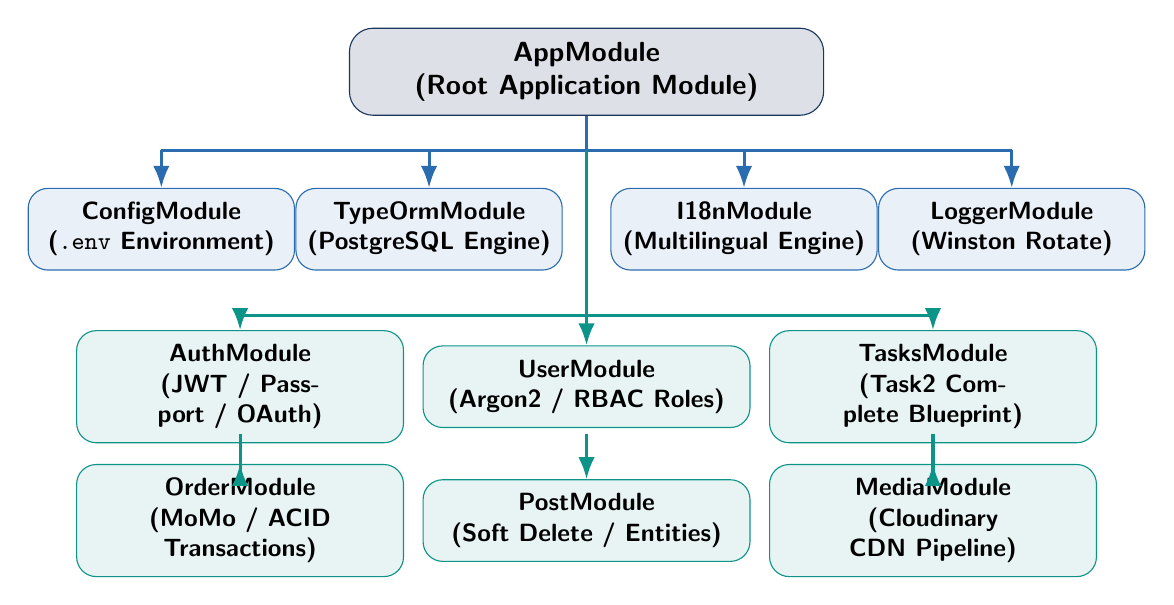
\begin{tikzpicture}[
      root/.style={rectangle, draw=primary, fill=primary!15, rounded corners=3mm, text centered, minimum height=1.1cm, text width=5.6cm, inner xsep=6pt, inner ysep=5pt, font=\normalsize\sffamily\bfseries},
      corebox/.style={rectangle, draw=secondary, fill=secondary!10, rounded corners=2.5mm, text centered, minimum height=1.0cm, text width=3.1cm, inner xsep=4pt, inner ysep=5pt, font=\small\sffamily\bfseries},
      featbox/.style={rectangle, draw=accent, fill=accent!10, rounded corners=2.5mm, text centered, minimum height=1.0cm, text width=3.8cm, inner xsep=5pt, inner ysep=5pt, font=\small\sffamily\bfseries},
      arrow/.style={-Latex, line width=1.1pt, color=secondary}
    ]
      % Root node at top
      \node (app) [root] at (0, 0) {AppModule\\(Root Application Module)};

      % Level 1: Core / Infrastructure Modules (y = -2.0)
      \node (config) [corebox] at (-5.4, -2.0) {ConfigModule\\(\texttt{.env} Environment)};
      \node (typeorm) [corebox] at (-2.0, -2.0) {TypeOrmModule\\(PostgreSQL Engine)};
      \node (i18n) [corebox] at (2.0, -2.0) {I18nModule\\(Multilingual Engine)};
      \node (logger) [corebox] at (5.4, -2.0) {LoggerModule\\(Winston Rotate)};

      % Level 2a: Feature Core Services (y = -4.0)
      \node (auth) [featbox] at (-4.4, -4.0) {AuthModule\\(JWT / Passport / OAuth)};
      \node (user) [featbox] at (0, -4.0) {UserModule\\(Argon2 / RBAC Roles)};
      \node (tasks) [featbox] at (4.4, -4.0) {TasksModule\\(Task2 Complete Blueprint)};

      % Level 2b: Feature Business Services (y = -5.7)
      \node (order) [featbox] at (-4.4, -5.7) {OrderModule\\(MoMo / ACID Transactions)};
      \node (post) [featbox] at (0, -5.7) {PostModule\\(Soft Delete / Entities)};
      \node (media) [featbox] at (4.4, -5.7) {MediaModule\\(Cloudinary CDN Pipeline)};

      % Clean distribution bus from AppModule to Core Modules
      \draw [line width=1.1pt, color=secondary] (app.south) -- (0, -1.0);
      \draw [line width=1.1pt, color=secondary] (-5.4, -1.0) -- (5.4, -1.0);
      \draw [arrow] (-5.4, -1.0) -- (config.north);
      \draw [arrow] (-2.0, -1.0) -- (typeorm.north);
      \draw [arrow] (2.0, -1.0) -- (i18n.north);
      \draw [arrow] (5.4, -1.0) -- (logger.north);

      % Clean distribution bus to Feature Modules (Level 2a)
      \draw [line width=1.1pt, color=accent] (0, -1.0) -- (0, -3.1);
      \draw [line width=1.1pt, color=accent] (-4.4, -3.1) -- (4.4, -3.1);
      \draw [arrow, color=accent] (-4.4, -3.1) -- (auth.north);
      \draw [arrow, color=accent] (0, -3.1) -- (user.north);
      \draw [arrow, color=accent] (4.4, -3.1) -- (tasks.north);

      % Clean distribution bus to Feature Modules (Level 2b)
      \draw [line width=1.1pt, color=accent] (-4.4, -4.6) -- (-4.4, -5.1);
      \draw [line width=1.1pt, color=accent] (0, -4.6) -- (0, -5.1);
      \draw [line width=1.1pt, color=accent] (4.4, -4.6) -- (4.4, -5.1);
      \draw [arrow, color=accent] (-4.4, -5.1) -- (order.north);
      \draw [arrow, color=accent] (0, -5.1) -- (post.north);
      \draw [arrow, color=accent] (4.4, -5.1) -- (media.north);
    \end{tikzpicture}
  }
  \caption{Sơ đồ cây phụ thuộc Module phân tầng chuẩn mực trong NestJS Enterprise}
  \label{fig:module-tree-pedagogy}
\end{figure}

Một nguyên lý tối quan trọng trong NestJS là \textbf{Ranh giới đóng gói}: Nếu Module A muốn sử dụng \texttt{UserService} của \texttt{UserModule}, thì \texttt{UserModule} bắt buộc phải liệt kê \texttt{UserService} trong mảng \texttt{exports: [UserService]}, và Module A phải đưa \texttt{UserModule} vào mảng \texttt{imports: [UserModule]}. Cơ chế này ngăn chặn việc truy cập tùy tiện xuyên module, buộc kỹ sư phải suy nghĩ kỹ càng về API công khai của từng phân hệ.

\section{Cơ Chế TypeScript Metadata Reflection}
Trọng tâm sức mạnh của NestJS nằm ở cơ chế **Decorators** kết hợp với thư viện \texttt{reflect-metadata}. Trong TypeScript, Decorator thực chất là một hàm bậc cao (\textit{Higher-Order Function}) được trình biên dịch thực thi ngay khi định nghĩa lớp, phương thức, thuộc tính hoặc tham số:
\begin{equation}
  \text{Decorator}(T) \longrightarrow \text{Reflect.defineMetadata}(\text{key}, \text{value}, T)
\end{equation}

Khi tùy chọn \texttt{"emitDecoratorMetadata": true} được kích hoạt trong \texttt{tsconfig.json}, trình biên dịch TypeScript (\texttt{tsc}) sẽ tự động phân tích cú pháp kiểu dữ liệu và phát sinh 3 khóa metadata tiêu chuẩn vào bytecode JavaScript:
\begin{itemize}
  \item \texttt{design:type}: Kiểu dữ liệu của thuộc tính hoặc trường được chú thích.
  \item \texttt{design:paramtypes}: Mảng các kiểu dữ liệu của tham số đầu vào trong constructor hoặc phương thức.
  \item \texttt{design:returntype}: Kiểu dữ liệu trả về của phương thức.
\end{itemize}

Nhờ \texttt{design:paramtypes}, khi kỹ sư viết:
\begin{codebox}[Ví dụ constructor injection qua metadata]
\begin{Verbatim}[fontsize=\small]
@Injectable()
export class TasksService {
  constructor(
    @InjectRepository(TaskEntity)
    private readonly tasksRepository: Repository<TaskEntity>,
  ) {}
}
\end{Verbatim}
\end{codebox}
NestJS không cần kỹ sư phải cấu hình thủ công chuỗi token định danh. IoC Container sử dụng \texttt{Reflect.getMetadata('design:paramtypes', TasksService)} để đọc trực tiếp các tham số và tự động tiêm (\textit{inject}) đúng instance của \texttt{Repository<TaskEntity>} vào thời điểm khởi động.

\section{So Sánh Toàn Diện: NestJS vs Express Thuần vs Fastify}

\begin{table}[htbp]
  \centering
  \small
  \caption{So sánh chuyên sâu giữa NestJS, Express thuần và Fastify}
  \label{tab:framework-comparison}
  \begin{tabularx}{\textwidth}{l p{3.2cm} p{3.2cm} X}
    \toprule
    \textbf{Tiêu chí} & \textbf{NestJS (Dự án)} & \textbf{Express thuần} & \textbf{Fastify thuần} \\
    \midrule
    Kiến trúc tổ chức & Mô-đun hóa, DDD, chuẩn doanh nghiệp. & Tự do hoàn toàn, dễ phân mảnh. & Dựa trên Schema, có hỗ trợ plugin. \\
    Dependency Injection & Tích hợp sẵn IoC Container mạnh mẽ. & Không có (phải cài thư viện ngoài). & Không có tích hợp sẵn. \\
    Type Safety & TypeScript hạng nhất, DTO validation. & JavaScript thuần (phải tự tích hợp). & Hỗ trợ schema qua JSON Schema. \\
    Tự động hóa Swagger & Tự động sinh từ DTO và Decorators. & Viết file YAML/JSON thủ công. & Có plugin fastify-swagger. \\
    Khả năng kiểm thử & Cực kỳ dễ dàng qua TestingModule & Phải monkey-patch hoặc mock thủ công. & Hỗ trợ inject HTTP request test. \\
    \bottomrule
  \end{tabularx}
\end{table}

\section{Kiến Trúc Phân Tầng Chuyên Sâu Của Dự Án}
Hệ thống mã nguồn thực nghiệm \texttt{c:\textbackslash Users\textbackslash LAPTOP\textbackslash nest} được thiết kế theo mô hình phân tầng chặt chẽ:

\begin{figure}[htbp]
  \centering
  \resizebox{0.95\textwidth}{!}{
    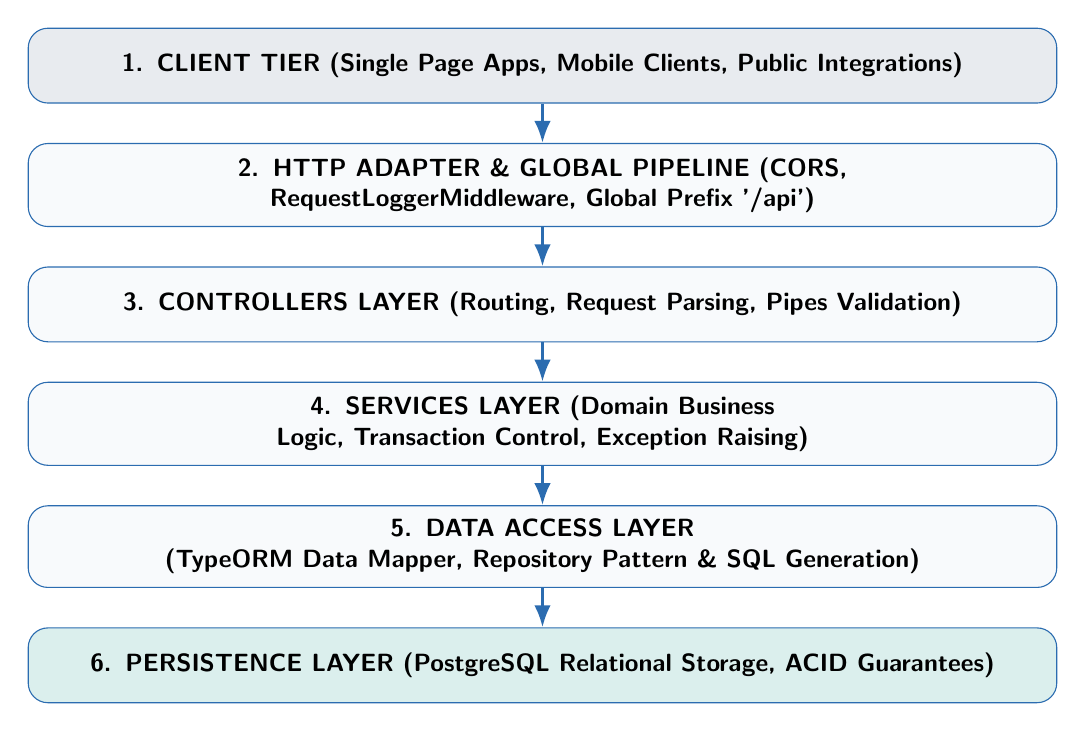
\begin{tikzpicture}[
      box/.style={rectangle, draw=secondary, fill=codebg, rounded corners=2.5mm, text centered, minimum height=0.95cm, text width=12.5cm, inner xsep=8pt, inner ysep=5pt, font=\bfseries\small\sffamily},
      arrow/.style={-Latex, line width=1.1pt, color=secondary}
    ]
      \node (client) [box, fill=primary!10] {1. CLIENT TIER (Single Page Apps, Mobile Clients, Public Integrations)};
      \node (gw) [box, below=0.5cm of client] {2. HTTP ADAPTER \& GLOBAL PIPELINE (CORS, RequestLoggerMiddleware, Global Prefix '/api')};
      \node (ctrl) [box, below=0.5cm of gw] {3. CONTROLLERS LAYER (Routing, Request Parsing, Pipes Validation)};
      \node (svc) [box, below=0.5cm of ctrl] {4. SERVICES LAYER (Domain Business Logic, Transaction Control, Exception Raising)};
      \node (repo) [box, below=0.5cm of svc] {5. DATA ACCESS LAYER\\(TypeORM Data \mbox{Mapper}, Repository Pattern \& SQL Generation)};
      \node (db) [box, fill=accent!15, below=0.5cm of repo] {6. PERSISTENCE LAYER (PostgreSQL Relational Storage, ACID Guarantees)};

      \draw [arrow] (client) -- (gw);
      \draw [arrow] (gw) -- (ctrl);
      \draw [arrow] (ctrl) -- (svc);
      \draw [arrow] (svc) -- (repo);
      \draw [arrow] (repo) -- (db);
    \end{tikzpicture}
  }
  \caption{Mô hình phân tầng kiến trúc 6 lớp trong NestJS Enterprise}
  \label{fig:layered-arch}
\end{figure}

Dữ liệu di chuyển theo **Luồng Một Chiều (Unidirectional Data Flow)**: Yêu cầu từ Client đi tuần tự từ trên xuống dưới, và kết quả từ cơ sở dữ liệu được bao bọc ngược trở lại lên trên. Tầng dưới tuyệt đối không được gọi ngược trực tiếp lên tầng trên, bảo đảm tính độc lập và khả năng bảo trì tối đa.

\section{Giải Phẫu Chu Trình Bootstrap Khởi Động Tại \texttt{src/main.ts}}
Tệp tin \texttt{src/main.ts} là điểm nhập cảnh duy nhất (\textit{Single Entry Point}) của ứng dụng. Hãy giải phẫu chi tiết mã nguồn khởi động thực tế của dự án:

\begin{codebox}[Mã nguồn khởi động lõi trong src/main.ts]
\begin{Verbatim}[fontsize=\small]
import { ValidationPipe } from '@nestjs/common';
import { NestFactory } from '@nestjs/core';
import { AppModule } from './app.module';
import { ProjectLogger } from '@core/loggers';
import { ConfigService } from '@nestjs/config';
import { requestLoggerMiddleware } from '@shared/middleware/request-logger.middleware';
import { setupSwagger } from './setup-swagger';
import { ExpressAdapter, NestExpressApplication } from '@nestjs/platform-express';

const logger = new ProjectLogger('bootstrap');

async function bootstrap(): Promise<NestExpressApplication> {
  // 1. Khởi tạo ứng dụng với Express Adapter và bật CORS
  const app = await NestFactory.create<NestExpressApplication>(
    AppModule,
    new ExpressAdapter(),
    { cors: true },
  );

  // 2. Thiết lập tiền tố URL toàn cục: Mọi route đều bắt đầu bằng /api
  app.setGlobalPrefix('/api');

  // 3. Đăng ký Middleware ghi log toàn cục
  app.use(requestLoggerMiddleware);
  app.enableCors();

  // 4. Kích hoạt đường ống thẩm định DTO toàn cục
  app.useGlobalPipes(
    new ValidationPipe({
      whitelist: true,
      stopAtFirstError: true,
      transform: true,
    }),
  );

  // 5. Khởi tạo hệ thống tài liệu tương tác Swagger OpenAPI
  setupSwagger(app);

  // 6. Đăng ký Middleware xử lý tiêu đề CORS nâng cao
  app.use((req, res, next) => {
    res.header('Access-Control-Allow-Origin', '*');
    res.header('Access-Control-Allow-Methods', 'GET,PUT,POST,DELETE');
    res.header('Access-Control-Allow-Headers', 'Content-Type, Accept');
    next();
  });

  // 7. Lấy cổng lắng nghe từ ConfigService và mở cổng kết nối
  const config = app.get<ConfigService>(ConfigService);
  await app.listen(config.get('PORT'), async () => {
    logger.info(`Application is running on: ${await app.getUrl()}`);
  });

  return app;
}
bootstrap();
\end{Verbatim}
\end{codebox}

\begin{infobox}[Ý Nghĩa Của Từng Bước Trong Chu Trình Khởi Động]
  \begin{enumerate}
    \item \textbf{CORS Configuration}: Dự án áp dụng cấu hình kép: vừa qua tùy chọn khởi tạo \texttt{\{ cors: true \}}, vừa qua middleware thiết lập tường minh các headers (\texttt{Access-Control-Allow-Origin}, \texttt{Methods}, \texttt{Headers}) nhằm bảo đảm khả năng tích hợp trơn tru với các Single Page Applications (React, Vue, Angular) chạy trên các domain khác nhau.
    \item \textbf{Global Prefix \texttt{'/api'}}: Chuẩn hóa không gian tên cho mọi API backend, giúp phân biệt rõ ràng giữa các route nghiệp vụ và các route hệ thống (như giao diện Swagger tại \texttt{/docs} hoặc health check).
    \item \textbf{ConfigService Discovery}: Thay vì đọc trực tiếp biến môi trường qua \texttt{process.env.PORT} vốn dễ gây lỗi thời gian chạy nếu biến chưa nạp, ứng dụng trích xuất \texttt{ConfigService} trực tiếp từ IoC Container thông qua \texttt{app.get<ConfigService>(ConfigService)} để bảo đảm tính an toàn kiểu dữ liệu.
  \end{enumerate}
\end{infobox}

% ==================== CHƯƠNG 2 ====================
\chapter{Inversion of Control (IoC) \& Dependency Injection Chuyên Sâu}

\section{Nguyên Lý Đảo Ngược Phụ Thuộc (Dependency Inversion)}
Trong thiết kế phần mềm hướng đối tượng theo bộ nguyên lý SOLID, chữ **D** đại diện cho **Dependency Inversion Principle (DIP)**:
\begin{quote}
  \textit{"Các module cấp cao không nên phụ thuộc vào các module cấp thấp. Cả hai nên phụ thuộc vào sự trừu tượng (Abstraction). Sự trừu tượng không nên phụ thuộc vào chi tiết, mà chi tiết phải phụ thuộc vào sự trừu tượng."}
\end{quote}

Khi một lớp tự khởi tạo đối tượng phụ thuộc của nó bằng từ khóa \texttt{new}:
\begin{codebox}[Mã nguồn liên kết chặt chẽ - Phản mẫu thiết kế (Anti-pattern)]
\begin{Verbatim}[fontsize=\small]
export class TasksService {
  private repository: TaskRepository;
  constructor() {
    this.repository = new PostgresTaskRepository(); // LIÊN KẾT CHẶT!
  }
}
\end{Verbatim}
\end{codebox}
Lớp \texttt{TasksService} bị "cột chặt" vào triển khai cụ thể của PostgreSQL. Kỹ sư không thể nào thay thế kho lưu trữ này bằng một Mock Repository khi viết Unit Test mà không phải sửa mã nguồn gốc!

NestJS hiện thực hóa hoàn chỉnh mô hình **Inversion of Control (IoC)**: Lập trình viên chỉ cần khai báo kiểu dữ liệu cần thiết trong constructor, việc khởi tạo, giải quyết thứ tự phụ thuộc và truyền instance vào sẽ do **IoC Container** phụ trách hoàn toàn:

\begin{figure}[htbp]
  \centering
  \resizebox{0.95\textwidth}{!}{
    \begin{tikzpicture}[
      box/.style={rectangle, draw=secondary, fill=codebg, rounded corners=2.5mm, text centered, minimum height=1.1cm, text width=4.4cm, inner xsep=6pt, inner ysep=5pt, font=\small\sffamily},
      container/.style={rectangle, draw=primary, fill=primary!8, rounded corners=3mm, text centered, minimum height=3.6cm, text width=5.6cm, inner xsep=6pt, inner ysep=6pt, font=\bfseries\small\sffamily},
      lbl/.style={fill=white, draw=secondary!40, rounded corners=1.5mm, inner sep=3pt, font=\scriptsize\bfseries\sffamily},
      arrow/.style={-Latex, line width=1.1pt, color=secondary}
    ]
      \node (ioc) [container] at (0, 0) {NestJS IoC Container\\(Registry, Scopes\\\& Life-Cycle Internals)};
      \node (repo) [box] at (-8.8, 0) {TypeORM Repository\\(\texttt{@InjectRepository})};
      \node (svc) [box] at (8.8, 0) {Domain Service\\(\texttt{@Injectable})};
      \node (ctrl) [box] at (8.8, -2.8) {REST Controller\\(\texttt{@Controller})};

      \draw [arrow] (repo.east) -- node[lbl, above=1.5mm] {1. Đăng ký Provider} (ioc.west);
      \draw [arrow] (ioc.east) -- node[lbl, above=1.5mm] {2. Inject Singleton Instance} (svc.west);
      \draw [arrow] (svc.south) -- node[lbl, right=2mm] {3. Inject Service Instance} (ctrl.north);
    \end{tikzpicture}
  }
  \caption{Sơ đồ luồng giải quyết phụ thuộc qua NestJS IoC Container}
  \label{fig:ioc-flow}
\end{figure}

\section{Cơ Chế Bên Dưới Của IoC Container (Container Internals)}
Khi ứng dụng NestJS boot, IoC Container thực hiện chu trình giải quyết phụ thuộc 3 pha:
\begin{enumerate}
  \item \textbf{Pha Đăng Ký (Registration Phase)}: Quét toàn bộ các Module và nạp định nghĩa của các Provider vào một bảng đăng ký nội bộ (\textit{Internal Registry}).
  \item \textbf{Pha Xây Dựng Đồ Thị (Graph Resolution Phase)}: Sử dụng giải thuật sắp xếp topo (\textit{Topological Sort}) trên cây phụ thuộc để phát hiện chu trình vòng lặp và xác định thứ tự khởi tạo chính xác từ các lá (leaf nodes) lên gốc.
  \item \textbf{Pha Cấp Phát Thực Thể (Instantiation Phase)}: Khởi tạo các instance theo đúng thứ tự topo, lưu trữ các Singleton vào bộ nhớ đệm (\textit{Singleton Cache} dạng \texttt{Map<Token, Instance>}) và tiêm vào các consumer tương ứng.
\end{enumerate}

\section{Bốn Cú Pháp Khai Báo Custom Providers}
Bên cạnh cú pháp khai báo rút gọn \texttt{providers: [TasksService]}, NestJS hỗ trợ 4 dạng khai báo tường minh chuyên sâu:
\begin{enumerate}
  \item \textbf{useClass}: Dùng để hoán đổi triển khai động theo môi trường (ví dụ môi trường test dùng MockService, môi trường production dùng RealService).
\begin{codebox}[Khai báo useClass hoán đổi môi trường]
\begin{Verbatim}[fontsize=\small]
{
  provide: TasksService,
  useClass: process.env.NODE_ENV === 'test' ? MockTasksService : TasksService,
}
\end{Verbatim}
\end{codebox}
  \item \textbf{useValue}: Dùng để inject các đối tượng tĩnh, hằng số cấu hình, hoặc mock object vào cây phụ thuộc mà không cần khởi tạo class.
\begin{codebox}[Khai báo useValue cho đối tượng cấu hình]
\begin{Verbatim}[fontsize=\small]
{
  provide: 'APP_CONFIG',
  useValue: Object.freeze({ timeout: 5000, maxRetries: 3 }),
}
\end{Verbatim}
\end{codebox}
  \item \textbf{useFactory}: Cho phép khởi tạo Provider một cách bất đồng bộ hoặc phụ thuộc vào kết quả tính toán từ các Provider khác (rất phổ biến khi khởi tạo kết nối database hoặc SDK bên thứ ba như Cloudinary hay Redis).
\begin{codebox}[Khai báo useFactory bất đồng bộ]
\begin{Verbatim}[fontsize=\small]
{
  provide: 'REDIS_CLIENT',
  useFactory: async (configService: ConfigService) => {
    const client = new Redis(configService.get('REDIS_URL'));
    await client.connect();
    return client;
  },
  inject: [ConfigService],
}
\end{Verbatim}
\end{codebox}
  \item \textbf{useExisting}: Tạo ra một bí danh (\textit{alias}) trỏ tới một provider đã tồn tại mà không khởi tạo thêm phiên bản mới.
\begin{codebox}[Khai báo useExisting làm bí danh]
\begin{Verbatim}[fontsize=\small]
{
  provide: 'ITasksService',
  useExisting: TasksService,
}
\end{Verbatim}
\end{codebox}
\end{enumerate}

\section{Phân Tích Chuyên Sâu 3 Injection Scopes}
Mặc định trong NestJS, mọi provider đều hoạt động dưới dạng **Singleton** (\texttt{Scope.DEFAULT}). Đối tượng chỉ được khởi tạo một lần duy nhất lúc máy chủ khởi động và dùng chung cho toàn bộ các request:

\begin{table}[htbp]
  \centering
  \small
  \caption{So sánh 3 Injection Scopes trong NestJS}
  \label{tab:scopes-detailed}
  \begin{tabularx}{\textwidth}{l p{3cm} X}
    \toprule
    \textbf{Scope} & \textbf{Vòng đời thực thể} & \textbf{Phân tích ứng dụng trong dự án} \\
    \midrule
    \texttt{Scope.DEFAULT} & Khởi tạo duy nhất 1 lần (Singleton). Dùng chung cho toàn bộ requests. & Áp dụng cho 99\% các services (\texttt{TasksService}, \texttt{UserService}). Tối ưu hóa bộ nhớ RAM và CPU tối đa. \\
    \texttt{Scope.REQUEST} & Tạo mới instance cho mỗi HTTP request đi vào và tự hủy sau khi phản hồi. & Áp dụng tại \texttt{PaymentFactory} (\texttt{@Injectable(\{ scope: Scope.REQUEST \})}) khi cần lưu giữ ngữ cảnh phiên thanh toán riêng biệt. \\
    \texttt{Scope.TRANSIENT} & Một instance mới được tạo mỗi khi có một class khác inject nó vào. & Sử dụng cho các tiện ích loggers hoặc helper độc lập giữa các consumer. \\
    \bottomrule
  \end{tabularx}
\end{table}

\section{Hiệu Ứng Lan Truyền (Bubble-up Effect) Của \texttt{Scope.REQUEST}}
Trong dự án, tại \texttt{src/modules/order/factories/payment.factory.ts}, lớp \texttt{PaymentFactory} được đánh dấu rõ:
\begin{codebox}[PaymentFactory với Scope.REQUEST]
\begin{Verbatim}[fontsize=\small]
@Injectable({ scope: Scope.REQUEST })
export class PaymentFactory { ... }
\end{Verbatim}
\end{codebox}

\begin{warningbox}[Hiệu Ứng Lan Truyền (Bubble-up Effect) của Scope.REQUEST]
  Nếu Service A có \texttt{Scope.REQUEST}, bất kỳ Controller hoặc Service B nào inject Service A cũng sẽ tự động bị nâng lên thành \texttt{Scope.REQUEST}!
  
  Điều này dẫn tới hiện tượng **Áp Lực Dọn Rác (Garbage Collection Churn)**: Với mỗi request gửi đến, Node.js V8 Engine phải liên tục cấp phát bộ nhớ heap cho hàng loạt đối tượng mới, sau đó thu hồi khi request kết thúc. Trong các bài kiểm tra tải cao (Load Testing), việc lạm dụng \texttt{Scope.REQUEST} có thể khiến thông lượng xử lý sụt giảm từ 20,000 req/sec xuống dưới 4,000 req/sec và làm tăng độ trễ p99! Kỹ sư chỉ nên dùng Scope.REQUEST khi thực sự cần lưu giữ ngữ cảnh phiên (như Transaction Context hoặc Multi-tenancy Isolation).
\end{warningbox}

\section{Xử Lý Phụ Thuộc Vòng (Circular Dependency) Với \texttt{forwardRef()}}
Khi Service A inject Service B, và đồng thời Service B lại cần inject Service A, NestJS sẽ gặp tình trạng "con gà và quả trứng" khi dựng cây phụ thuộc. Để giải quyết, ta sử dụng hàm bao bọc tham chiếu trễ \texttt{forwardRef()}:
\begin{codebox}[Giải quyết Circular Dependency với forwardRef]
\begin{Verbatim}[fontsize=\small]
@Injectable()
export class UsersService {
  constructor(
    @Inject(forwardRef(() => AuthService))
    private readonly authService: AuthService,
  ) {}
}
\end{Verbatim}
\end{codebox}
Cơ chế này cũng áp dụng tương tự ở cấp Module thông qua \texttt{imports: [forwardRef(() => AuthModule)]}.

\section{Bốn Hooks Vòng Đời Của Ứng Dụng \& Cơ Chế Graceful Shutdown}
NestJS cung cấp bộ 4 hooks cho phép can thiệp vào các giai đoạn khởi tạo và dọn dẹp hệ thống:
\begin{itemize}
  \item \texttt{OnModuleInit}: Được gọi ngay khi các phụ thuộc của module đã được giải quyết xong. Thường dùng để khởi tạo kết nối mạng ngoại vi hoặc nạp cache khởi động.
  \item \texttt{OnApplicationBootstrap}: Được kích hoạt sau khi toàn bộ cây ứng dụng đã boot xong và chuẩn bị mở cổng mạng đón request.
  \item \texttt{OnModuleDestroy}: Được kích hoạt khi module nhận tín hiệu chuẩn bị hủy bỏ.
  \item \texttt{BeforeApplicationShutdown}: Cho phép thực hiện các thao tác đóng kết nối database an toàn (\textit{Graceful Shutdown}), giải phóng socket và hoàn tất các tác vụ nền đang xử lý dở dang trước khi tiến trình Node.js kết thúc:
\end{itemize}

\begin{codebox}[Hiện thực hóa Graceful Shutdown với BeforeApplicationShutdown]
\begin{Verbatim}[fontsize=\small]
@Injectable()
export class DatabaseService implements BeforeApplicationShutdown {
  constructor(private readonly dataSource: DataSource) {}

  async beforeApplicationShutdown(signal?: string) {
    console.log(`[Graceful Shutdown] Nhận tín hiệu ${signal}. Đang đóng hồ kết nối database...`);
    if (this.dataSource.isInitialized) {
      await this.dataSource.destroy();
      console.log('[Graceful Shutdown] Hồ kết nối PostgreSQL đã đóng an toàn.');
    }
  }
}
\end{Verbatim}
\end{codebox}
Để kích hoạt các hooks tắt máy này, trong \texttt{main.ts} cần bổ sung lệnh \texttt{app.enableShutdownHooks()} để lắng nghe các tín hiệu hệ điều hành POSIX như \texttt{SIGTERM} hoặc \texttt{SIGINT}.

% ==================== CHƯƠNG 3 ====================
\chapter[Chu Trình Sống 12 Bước Của HTTP Request]{Chu Trình Sống 12 Bước Của HTTP Request\\Trong Hệ Thống}

\section{Đường Ống Xử Lý Yêu Cầu (The Request Lifecycle Pipeline)}
Khi một yêu cầu HTTP được gửi từ phía máy khách đến máy chủ NestJS, nó không đi thẳng vào Controller mà phải đi qua một chuỗi các trạm kiểm soát nghiêm ngặt theo thứ tự tuần tự:

\begin{figure}[htbp]
  \centering
  \resizebox{0.95\textwidth}{!}{
    \begin{tikzpicture}[
      stepbox/.style={rectangle, draw=secondary, fill=codebg, rounded corners=2.5mm, text centered, minimum height=0.8cm, text width=12.5cm, inner xsep=8pt, inner ysep=4.5pt, font=\small\sffamily},
      arrow/.style={-Latex, line width=1.1pt, color=secondary}
    ]
      \node (s1) [stepbox, fill=primary!12] {1. TCP Connection \& Underlying HTTP Server (Node.js Express Engine)};
      \node (s2) [stepbox, below=0.45cm of s1] {2. Global Middlewares (RequestLoggerMiddleware đo Response Time \& IP)};
      \node (s3) [stepbox, below=0.45cm of s2] {3. Global Routing Matcher (Kiểm tra tiền tố URL toàn cục '/api')};
      \node (s4) [stepbox, below=0.45cm of s3] {4. Guards Pipeline (AuthGuard kiểm tra JWT, RolesGuard kiểm tra RBAC)};
      \node (s5) [stepbox, below=0.45cm of s4] {5. Interceptors (Pre-controller: Biến đổi request, ghi nhận thời gian bắt đầu)};
      \node (s6) [stepbox, below=0.45cm of s5] {6. Pipes (Global ValidationPipe kiểm tra DTO, ParseUUIDPipe kiểm tra ID)};
      \node (s7) [stepbox, fill=accent!15, below=0.45cm of s6] {7. Controller Action Execution (Định tuyến phương thức xử lý)};
      \node (s8) [stepbox, fill=accent!25, below=0.45cm of s7] {8. Service Business Logic (Thực thi quy tắc nghiệp vụ, kiểm tra ràng buộc)};
      \node (s9) [stepbox, below=0.45cm of s8] {9. Data Access Tier (TypeORM phát sinh SQL, thực thi trên PostgreSQL)};
      \node (s10) [stepbox, below=0.45cm of s9] {10. Interceptors (Post-controller: Biến đổi kết quả, chuẩn hóa định dạng trả về)};
      \node (s11) [stepbox, fill=warning!15, below=0.45cm of s10] {11. Exception Filters (Bắt giữ ngoại lệ Http/System, chuyển thành JSON RFC)};
      \node (s12) [stepbox, fill=success!15, below=0.45cm of s11] {12. HTTP Server Response (Gửi gói tin phản hồi HTTP về Client)};

      \draw [arrow] (s1) -- (s2);
      \draw [arrow] (s2) -- (s3);
      \draw [arrow] (s3) -- (s4);
      \draw [arrow] (s4) -- (s5);
      \draw [arrow] (s5) -- (s6);
      \draw [arrow] (s6) -- (s7);
      \draw [arrow] (s7) -- (s8);
      \draw [arrow] (s8) -- (s9);
      \draw [arrow] (s9) -- (s10);
      \draw [arrow] (s10) -- (s11);
      \draw [arrow] (s11) -- (s12);
    \end{tikzpicture}
  }
  \caption{Toàn cảnh chu trình sống 12 bước của một HTTP Request trong NestJS}
  \label{fig:lifecycle-12}
\end{figure}

\section{Phân Biệt Rạch Ròi Vai Trò Của Các Thành Phần Pipeline}
Nhiều kỹ sư khi mới tiếp cận NestJS thường nhầm lẫn giữa Middleware, Guard, Interceptor và Pipe. Hãy phân định rạch ròi trách nhiệm của từng thành phần:
\begin{itemize}
  \item \textbf{Middlewares}: Có thể truy cập đối tượng thô \texttt{req}, \texttt{res}, \texttt{next}. Hoàn toàn không biết Controller hay Action nào sẽ được gọi phía sau. Thích hợp cho ghi log toàn cục, nén dữ liệu gzip, thiết lập CORS.
  \item \textbf{Guards}: Trả lời câu hỏi duy nhất: \textbf{"Request này có được phép đi tiếp không?"}. Có quyền truy cập \texttt{ExecutionContext} và đọc metadata từ Decorators. Chuyên xử lý xác thực (Authentication) và phân quyền (Authorization).
  \item \textbf{Interceptors}: Kế thừa tư tưởng Lập trình hướng khía cạnh (\textit{Aspect-Oriented Programming - AOP}). Bao bọc việc thực thi của hàm xử lý bằng RxJS \texttt{Observable}. Có thể can thiệp trước và sau khi Controller chạy, dùng để đo lường hiệu năng, ghi cache hoặc biến đổi cấu trúc dữ liệu trả về.
  \item \textbf{Pipes}: Trả lời câu hỏi: \textbf{"Dữ liệu truyền vào có đúng kiểu và hợp lệ không?"}. Chuyên trách thẩm định (\textit{Validation}) và biến đổi kiểu (\textit{Transformation}).
  \item \textbf{Exception Filters}: Trả lời câu hỏi: \textbf{"Khi có lỗi xảy ra, cấu trúc phản hồi lỗi gửi về Client sẽ như thế nào?"}. Bắt mọi ngoại lệ chưa được xử lý và định dạng thành JSON chuẩn.
\end{itemize}

\section{Cơ Chế Đa Giao Thức: \texttt{ExecutionContext} vs \texttt{ArgumentsHost}}
NestJS được thiết kế để có thể chạy trên nhiều nền tảng truyền thông khác nhau: HTTP REST, WebSocket, Microservices (gRPC, RabbitMQ, Kafka). Để các Guards, Interceptors và Exception Filters có thể tái sử dụng xuyên suốt các giao thức này mà không phải viết lại, NestJS cung cấp hai lớp trừu tượng:

\begin{enumerate}
  \item \textbf{\texttt{ArgumentsHost}}: Đóng vai trò là một wrapper bao bọc mảng tham số được truyền tới handler của nền tảng bên dưới:
\begin{codebox}[Trích xuất ngữ cảnh từ ArgumentsHost trong Exception Filter]
\begin{Verbatim}[fontsize=\small]
@Catch(NotFoundException)
export class NotFoundExceptionFilter implements ExceptionFilter {
  catch(exception: NotFoundException, host: ArgumentsHost) {
    const ctx = host.switchToHttp(); // Chuyển đổi sang ngữ cảnh HTTP
    const res = ctx.getResponse<Response>();
    const req = ctx.getRequest<Request>();
    res.status(404).json({ statusCode: 404, path: req.url });
  }
}
\end{Verbatim}
\end{codebox}
  Nếu ứng dụng chuyển sang chạy gRPC, kỹ sư chỉ cần gọi \texttt{host.switchToRpc().getData()} mà không làm thay đổi chữ ký của Exception Filter!
  \item \textbf{\texttt{ExecutionContext}}: Kế thừa trực tiếp từ \texttt{ArgumentsHost}, bổ sung thêm hai phương thức phản chiếu quan trọng:
    \begin{itemize}
      \item \texttt{context.getClass()}: Trả về tham chiếu tới lớp Controller đang thực thi.
      \item \texttt{context.getHandler()}: Trả về tham chiếu tới phương thức xử lý cụ thể.
    \end{itemize}
    Đây chính là chìa khóa để \texttt{RolesGuard} sử dụng \texttt{Reflector} nhằm trích xuất metadata do decorator \texttt{@Roles()} gắn vào, như chúng ta sẽ tìm hiểu chi tiết ở Chương 12.
\end{enumerate}

% ==================== CHƯƠNG 4 ====================
\chapter{Thẩm Định Dữ Liệu Với ValidationPipe \& DTO Pattern}

\section{Bảo Vệ Hệ Thống Trước Lỗ Hổng Mass Assignment}
Lỗ hổng bảo mật **Mass Assignment** (hay \textit{Over-posting Attack}) xảy ra khi ứng dụng tự động gán toàn bộ các thuộc tính người dùng gửi lên vào đối tượng lưu trữ cơ sở dữ liệu mà không qua tầng sàng lọc. 

Hãy tưởng tượng một người dùng độc hại gửi yêu cầu tạo bài viết hoặc đăng ký:
\begin{codebox}[Payload tấn công gửi kèm trường đặc quyền nguy hiểm]
\begin{Verbatim}[fontsize=\small]
{
  "title": "Hướng dẫn NestJS",
  "category": "Technology",
  "role": "ADMIN",            // TRƯỜNG TẤN CÔNG ĐẶC QUYỀN!
  "is_completed": true,
  "isSuperUser": true         // TRƯỜNG TẤN CÔNG ĐẶC QUYỀN!
}
\end{Verbatim}
\end{codebox}
Nếu Service gán thẳng \texttt{repository.save(req.body)}, đối tượng có thể bị ghi đè các cột đặc quyền hệ thống, biến người dùng thường thành Quản trị viên cấp cao!

NestJS dập tắt triệt để nguy cơ này nhờ mô hình kết hợp giữa **Data Transfer Object (DTO)** và **ValidationPipe**.

\section{Bộ Ba Cờ Cấu Hình Toàn Cục Trong \texttt{src/main.ts}}
Tại tệp khởi động \texttt{src/main.ts}, hệ thống kích hoạt ValidationPipe với bộ ba cấu hình chuẩn mực:

\begin{codebox}[Cấu hình ValidationPipe toàn cục chuẩn mực trong src/main.ts]
\begin{Verbatim}[fontsize=\small]
app.useGlobalPipes(
  new ValidationPipe({
    whitelist: true,
    stopAtFirstError: true,
    transform: true,
  }),
);
\end{Verbatim}
\end{codebox}

\begin{itemize}
  \item \textbf{whitelist: true}: Quét qua toàn bộ các thuộc tính của đối tượng gửi lên. Bất kỳ thuộc tính nào không có decorator thẩm định khai báo trong class DTO sẽ bị **loại bỏ hoàn toàn** trước khi đến tay Controller. Các trường độc hại như \texttt{role} hay \texttt{isSuperUser} ở trên sẽ bị gọt sạch ngay tại cửa ngõ!
  \item \textbf{transform: true}: Chuyển đổi payload từ dạng plain JavaScript object thành thể hiện thực sự (\textit{class instance}) của lớp DTO, cho phép các hàm phương thức, getter, và các decorator biến đổi của \texttt{class-transformer} hoạt động chuẩn xác.
  \item \textbf{stopAtFirstError: true}: Ngay khi phát hiện trường đầu tiên vi phạm ràng buộc, đường ống dừng thẩm định ngay lập tức và ném lỗi 400 Bad Request về Client, giúp tiết kiệm tối đa chu kỳ CPU của máy chủ dưới áp lực tải cao.
\end{itemize}

\section{Kế Thừa DTO Linh Hoạt Với \texttt{PartialType()}}
Để tuân thủ nguyên lý DRY (\textit{Don't Repeat Yourself}), NestJS cung cấp hàm tiện ích \texttt{PartialType()} từ thư viện \texttt{@nestjs/swagger} (hoặc \texttt{@nestjs/mapped-types}). Hãy khảo sát cách thức áp dụng thực tế trong hai module \texttt{post} và \texttt{tasks}:

\begin{codebox}[Kế thừa DTO trong src/modules/post/dto/ và tasks/dto/]
\begin{Verbatim}[fontsize=\small]
// 1. DTO tạo mới: Bắt buộc các trường
export class CreatePostDto {
  @IsString()
  @IsNotEmpty()
  title: string;

  @IsString()
  @IsNotEmpty()
  category: string;

  @IsString()
  @IsOptional()
  description?: string;
}

// 2. DTO cập nhật PATCH: Mọi trường tự động trở thành Optional
export class UpdatePostDto extends PartialType(CreatePostDto) {}
\end{Verbatim}
\end{codebox}

\begin{infobox}[Cơ Chế Phía Sau Của PartialType]
  Khi \texttt{UpdatePostDto} kế thừa \texttt{PartialType(CreatePostDto)}, thư viện sẽ tự động sao chép toàn bộ các quy tắc thẩm định (\texttt{@IsString()}, \texttt{@MaxLength()}...) nhưng gắn thêm decorator \texttt{@IsOptional()} cho từng trường, đồng thời cập nhật đúng metadata hiển thị cho Swagger UI. Kỹ sư không cần phải sao chép lặp lại mã nguồn của \texttt{CreatePostDto}!
\end{infobox}

\section{Phân Tách DTO Quản Trị Viên (Admin) \& Người Dùng Thường (Client)}
Trong các hệ thống phân quyền phức tạp, việc sử dụng chung một DTO cho cả thao tác của Quản trị viên và Khách hàng là một lỗ hổng thiết kế nguy hiểm:
\begin{itemize}
  \item \textbf{DTO Phía Client}: Thường bị hạn chế các trường nhạy cảm. Người dùng không được phép tự ý gán trạng thái phê duyệt (\texttt{status: 'APPROVED'}), gán vai trò (\texttt{role: 'ADMIN'}), hoặc sửa đổi điểm tích lũy.
  \item \textbf{DTO Phía Admin (\texttt{src/modules/admin/dto/create-post.dto.ts})}: Cho phép Quản trị viên chỉ định danh mục đặc biệt, phê duyệt trực tiếp hoặc gắn cờ ưu tiên.
\end{itemize}
Bằng cách chia tách thành các lớp DTO biệt lập kết hợp với cờ \texttt{whitelist: true}, hệ thống bảo đảm chắc chắn rằng người dùng thông thường không bao giờ có thể tự nâng quyền hoặc sửa đổi các thuộc tính đặc quyền của hệ thống.

\section{Chuyển Đổi Kiểu Tham Số URL Với \texttt{class-transformer}}
Trong giao thức HTTP, toàn bộ các tham số trên URL (query strings và route params) đều được máy chủ web nhận vào dưới dạng chuỗi thô (\textit{raw strings}). Ví dụ: \texttt{?page=2\&page\_size=10\&isCompleted=true}.

Nếu không có cơ chế chuyển đổi kiểu:
\begin{equation}
  \text{page} + 1 = \text{'2'} + 1 = \text{'21'} \quad (\text{Nối chuỗi thay vì phép cộng số học!})
\end{equation}
Trong \texttt{PageOptionsDto} (\texttt{src/core/pagination/dto/page-option.dto.ts}), dự án sử dụng decorator \texttt{@Type(() => Number)} để ép kiểu an toàn:
\begin{codebox}[Ép kiểu số học trong PageOptionsDto]
\begin{Verbatim}[fontsize=\small]
export class PageOptionsDto {
  @Type(() => Number)
  @IsInt()
  @Min(1)
  @IsOptional()
  readonly page?: number = 1;

  @Type(() => Number)
  @IsInt()
  @Min(1)
  @Max(50)
  @IsOptional()
  readonly page_size?: number = 10;
}
\end{Verbatim}
\end{codebox}

\section{Tích Hợp Giữa \texttt{ValidationPipe} \& \texttt{ErrorService}}
Khi dữ liệu gửi lên không vượt qua được bài kiểm tra, \texttt{ValidationPipe} phát sinh một mảng các đối tượng \texttt{ValidationError} chứa thông tin chi tiết:
\begin{codebox}[Cấu trúc đối tượng ValidationError từ class-validator]
\begin{Verbatim}[fontsize=\small]
{
  "property": "title",
  "value": "",
  "constraints": {
    "isNotEmpty": "title should not be empty",
    "isString": "title must be a string"
  }
}
\end{Verbatim}
\end{codebox}
Đối tượng này được ném ra dưới dạng \texttt{UnprocessableEntityException} hoặc \texttt{BadRequestException}. Bộ lọc ngoại lệ \texttt{UnprocessableEntityExceptionFilter} tại \texttt{src/core/filters/} sẽ bắt lấy lỗi này và chuyển tiếp tới \texttt{ErrorService} để tra cứu từ điển \texttt{src/i18n/vi/errors.json}, tự động dịch câu thông báo sang tiếng Việt và gắn tên trường bị vi phạm vào JSON phản hồi trả về cho máy khách.

% #############################################################
% #################### PHẦN II: DATABASE & TYPEORM ############
% #############################################################
\part{Tầng Dữ Liệu \& ORM Doanh Nghiệp Với TypeORM (Database Engineering)}

\chapter{Kiến Trúc Truy Cập Dữ Liệu Với TypeORM 0.3}

\section{Mẫu Thiết Kế Data Mapper vs Active Record}
Trong phát triển ứng dụng cơ sở dữ liệu hướng đối tượng, kiến trúc sư phần mềm Martin Fowler đã phân định hai mẫu thiết kế truy cập dữ liệu kinh điển:

\begin{itemize}
  \item \textbf{Active Record}: Thực thể (\textit{Entity}) kế thừa từ một lớp cơ sở (như \texttt{BaseEntity}) và tự chứa toàn bộ các phương thức truy vấn cơ sở dữ liệu (ví dụ: \texttt{task.save()}, \texttt{Task.find()}). Mặc dù cú pháp này có vẻ ngắn gọn, Active Record vi phạm nghiêm trọng **Nguyên Lý Trách Nhiệm Đơn Lẻ (Single Responsibility Principle)**: thực thể dữ liệu vừa phải chịu trách nhiệm mô hình hóa nghiệp vụ, vừa phải gánh vác trách nhiệm kết nối mạng và thực thi SQL. Điều này khiến việc viết Unit Test cho tầng Service trở nên bất khả thi nếu không có một cơ sở dữ liệu thật chạy ngầm!
  \item \textbf{Data Mapper (Dự án áp dụng)}: Thực thể chỉ đơn thuần là một cấu trúc dữ liệu thuần túy (\textit{Plain Data Holder}) chứa thuộc tính và metadata ánh xạ cột. Toàn bộ logic tương tác CSDL (tìm kiếm, chèn, xóa, cập nhật, phân trang) được chuyển giao hoàn toàn cho đối tượng **Repository** độc lập. Cách tiếp cận này tách biệt rạch ròi miền nghiệp vụ (\textit{Domain Model}) khỏi hạ tầng lưu trữ (\textit{Persistence Infrastructure}), tạo điều kiện lý tưởng để giả lập (\textit{mocking}) tầng dữ liệu khi viết kiểm thử tự động.
\end{itemize}

\section{Cấu Hình DataSource Tập Trung Trong TypeORM 0.3}
Trong phiên bản TypeORM 0.3, việc kết nối cơ sở dữ liệu đã chuyển đổi toàn diện từ phương thức toàn cục \texttt{createConnection} sang đối tượng quản lý tập trung **DataSource**. Hãy giải phẫu tệp cấu hình thực tế tại \texttt{src/database/typeorm/config.ts}:

\begin{codebox}[Mã nguồn cấu hình DataSource tập trung: src/database/typeorm/config.ts]
\begin{Verbatim}[fontsize=\small]
import fs from 'fs';
import { DataSource } from 'typeorm';
import { ConfigService } from '@nestjs/config';
import { config } from 'dotenv';
import entities from './entities';

config();
const configService = new ConfigService();

export const dataSource = new DataSource({
  type: 'postgres',
  host: configService.get('TYPEORM_HOST'),
  port: configService.get<number>('TYPEORM_PORT'),
  username: configService.get('TYPEORM_USERNAME'),
  password: configService.get('TYPEORM_PASSWORD'),
  database: configService.get('TYPEORM_DATABASE'),
  entities,
  ssl:
    configService.get('DB_USE_SSL') === 'true'
      ? {
          ca: fs.readFileSync('ca-certificate.crt'),
        }
      : undefined,
  migrations: ['src/database/typeorm/migrations/*.ts'],
});
\end{Verbatim}
\end{codebox}

\begin{infobox}[An Toàn Kết Nối Cơ Sở Dữ Liệu Với SSL CA]
  Trong môi trường doanh nghiệp điện toán đám mây (AWS RDS, Google Cloud SQL, Neon PostgreSQL), việc truyền dữ liệu qua kênh mạng công cộng bắt buộc phải mã hóa bằng Transport Layer Security (TLS/SSL). Dự án hỗ trợ cờ \texttt{DB\_USE\_SSL}: khi kích hoạt, hệ thống tự động nạp chứng chỉ gốc \texttt{ca-certificate.crt} để xác minh danh tính máy chủ cơ sở dữ liệu, chống lại hoàn toàn các cuộc tấn công nghe lén hoặc giả mạo (\textit{Man-in-the-Middle}).
\end{infobox}

\section{Quản Lý Hồ Kết Nối (Connection Pooling) \& Tải Cao}
Trong môi trường sản phẩm thực tế, việc mở một kết nối TCP/IP mới tới PostgreSQL cho mỗi truy vấn là một hành động vô cùng tốn kém tài nguyên: máy chủ CSDL phải khởi tạo tiến trình backend mới, thực hiện bắt tay SSL, xác thực quyền và cấp phát bộ nhớ đệm (\textit{work\_mem}).

TypeORM sử dụng thư viện \texttt{pg-pool} quản lý một hồ kết nối duy trì sẵn (\textit{Connection Pool}):
\begin{itemize}
  \item \textbf{max}: Giới hạn số lượng kết nối tối đa mở đồng thời tới cơ sở dữ liệu (mặc định 10 đến 20 kết nối). Việc giới hạn này bảo vệ PostgreSQL không bị quá tải CPU và cạn kiệt bộ nhớ khi có hàng chục nghìn request ập đến cùng lúc.
  \item \textbf{idleTimeoutMillis}: Thời gian tối đa một kết nối rảnh rỗi được giữ trong pool trước khi bị đóng (thường là 30,000ms), giải phóng tài nguyên cho hệ điều hành.
  \item \textbf{connectionTimeoutMillis}: Thời gian tối đa chờ đợi để mượn một kết nối từ pool trước khi ném ngoại lệ hết thời gian (\textit{Timeout Exception}).
\end{itemize}

\section{Nguy Cơ Tiềm Ẩn Của Cờ \texttt{synchronize: true}}
Nhiều lập trình viên khi mới học NestJS thường bật cờ \texttt{synchronize: true} trong cấu hình TypeORM để bảng CSDL tự động cập nhật khi sửa code Entity.

\begin{warningbox}[Quy Tắc Sống Còn: Tuyệt Đối Cấm synchronize: true Trên Môi Trường Production]
  Cờ \texttt{synchronize: true} thực hiện so sánh mã nguồn Entity với schema CSDL mỗi khi ứng dụng khởi động. Nếu bạn đổi tên một cột (ví dụ từ \texttt{title} sang \texttt{heading}) hoặc xóa một thuộc tính trong Entity, TypeORM sẽ ngay lập tức phát sinh lệnh \texttt{DROP COLUMN} hoặc \texttt{DROP TABLE}!
  
  Hành động này dẫn tới việc **MẤT DỮ LIỆU VĨNH VIỄN** của hàng triệu khách hàng mà không có cách nào cứu vãn. Trong môi trường Staging và Production của doanh nghiệp, \texttt{synchronize: false} là bắt buộc 100\%, và mọi thay đổi cấu trúc dữ liệu phải được thực hiện thông qua **TypeORM Migrations** có kiểm duyệt mã nguồn (*Code Review*).
\end{warningbox}

\section{Quản Lý Giao Dịch Dữ Liệu (Transactions) Với \texttt{QueryRunner}}
Trong các nghiệp vụ phức tạp đòi hỏi tính toàn vẹn tuyệt đối (như tạo đơn hàng, trừ tiền ví, cập nhật kho hàng), kỹ sư không thể thực hiện các câu lệnh \texttt{save()} rời rạc vì nếu bước sau thất bại, bước trước sẽ để lại dữ liệu rác.

TypeORM cung cấp đối tượng \texttt{QueryRunner} cho phép kiểm soát giao dịch theo chuẩn ACID:

\begin{codebox}[Mẫu giao dịch dữ liệu chuẩn mực với QueryRunner trong OrderService]
\begin{Verbatim}[fontsize=\small]
const queryRunner = this.datasource.createQueryRunner();
await queryRunner.connect();
await queryRunner.startTransaction();

try {
  // 1. Tạo đơn hàng trong ngữ cảnh Transaction
  const createdOrder = queryRunner.manager.create(Order, { ...orderData });
  const savedOrder = await queryRunner.manager.save(Order, createdOrder);

  // 2. Tạo chi tiết đơn hàng
  const details = queryRunner.manager.create(OrderDetails, { orderId: savedOrder.id });
  await queryRunner.manager.save(OrderDetails, details);

  // 3. Cam kết giao dịch vào CSDL
  await queryRunner.commitTransaction();
  return savedOrder;
} catch (error) {
  // 4. Nếu có bất kỳ lỗi nào, hoàn tác toàn bộ trạng thái ban đầu
  await queryRunner.rollbackTransaction();
  throw error;
} finally {
  // 5. BẮT BUỘC: Giải phóng kết nối trả lại cho Hồ kết nối (Connection Pool)
  await queryRunner.release();
}
\end{Verbatim}
\end{codebox}
Nếu thiếu khối lệnh \texttt{finally \{ await queryRunner.release(); \}}, kết nối cơ sở dữ liệu sẽ bị "treo" vĩnh viễn. Chỉ sau vài trăm request, hồ kết nối sẽ cạn kiệt (\textit{Connection Pool Exhaustion}), khiến toàn bộ máy chủ backend bị tê liệt hoàn toàn!

% ==================== CHƯƠNG 6 ====================
\chapter{Mô Hình Hóa Thực Thể \& Decorators Tùy Biến}

\section{Lớp Cơ Sở Trừu Tượng \texttt{AbstractEntity} \& Mẫu \texttt{toDto()}}
Để tuân thủ nguyên lý DRY (\textit{Don't Repeat Yourself}), dự án xây dựng lớp cơ sở \texttt{AbstractEntity} tại \texttt{src/shared/abstract.entity.ts}:

\begin{codebox}[Mã nguồn AbstractEntity trong src/shared/abstract.entity.ts]
\begin{Verbatim}[fontsize=\small]
import { AbstractDto } from './dto/abstract.dto';
import { Constructor } from './types/utility-types';

export interface IAbstractEntity<DTO extends AbstractDto, O = never> {
  toDto(options?: O): DTO;
}

export abstract class AbstractEntity<
  DTO extends AbstractDto = AbstractDto,
  O = never,
> implements IAbstractEntity<DTO, O> {
  private dtoClass?: Constructor<DTO, [AbstractEntity, O?]>;

  toDto(options?: O): DTO {
    const dtoClass = this.dtoClass;
    if (!dtoClass) {
      throw new Error(
        `You need to use @UseDto on class (${this.constructor.name}) be able to call toDto function`,
      );
    }
    return new dtoClass(this, options);
  }
}
\end{Verbatim}
\end{codebox}

Mô hình này mang lại sự bảo đảm an toàn dữ liệu: phương thức \texttt{toDto()} bắt buộc thực thể phải được ánh xạ qua lớp DTO phản hồi, ngăn chặn việc vô tình để lộ các trường nhạy cảm như \texttt{password}, \texttt{secretKey} hay các cờ logic nội bộ ra ngoài mạng Internet.

\section{Khóa Chính Toàn Cầu UUID v4 vs BigInt Auto-Increment}

\begin{table}[htbp]
  \centering
  \small
  \caption{So sánh chuyên sâu giữa UUID v4 và BigInt Auto-Increment}
  \label{tab:uuid-vs-bigint}
  \begin{tabularx}{\textwidth}{l p{4.5cm} X}
    \toprule
    \textbf{Tiêu chí} & \textbf{UUID v4 (Lựa chọn của dự án)} & \textbf{BigInt Auto-Increment} \\
    \midrule
    Tính bảo mật & \textbf{Tuyệt đối}: Không thể đoán trước ID bản ghi tiếp theo, triệt tiêu nguy cơ tấn công vét cạn ID (Insecure Direct Object Reference). & Yếu: ID tăng tuần tự (1, 2, 3...) giúp kẻ tấn công dễ dàng cào dữ liệu toàn bộ hệ thống. \\
    Khả năng phân tán & Sinh độc lập tại client hoặc server mà không bao giờ lo trùng lặp, tối ưu cho Sharding. & Phụ thuộc vào bộ đếm trung tâm của CSDL duy nhất. \\
    Kích thước lưu trữ & 16 bytes (128 bits), tốn dung lượng RAM chỉ mục hơn một chút. & 8 bytes (64 bits), nhỏ gọn. \\
    \bottomrule
  \end{tabularx}
\end{table}

\section{Chiến Lược Đặt Tên Tự Động (\texttt{SnakeNamingStrategy})}
JavaScript tuân theo quy ước đặt tên \textbf{camelCase} (ví dụ: \texttt{isCompleted}, \texttt{createdAt}), trong khi cơ sở dữ liệu quan hệ PostgreSQL chuẩn mực yêu cầu quy ước \textbf{snake\_case} (ví dụ: \texttt{is\_completed}, \texttt{created\_at}).

Nhờ cấu hình \texttt{SnakeNamingStrategy}, TypeORM tự động chuyển đổi qua lại giữa camelCase và snake\_case:
\begin{equation}
  \text{TaskEntity.isCompleted} \quad \xrightarrow{\text{SnakeNamingStrategy}} \quad \text{tasks.is\_completed}
\end{equation}
Lập trình viên không cần phải viết thủ công \texttt{@Column(\{ name: 'is\_completed' \})} lặp đi lặp lại trên từng thuộc tính, giúp mã nguồn luôn gọn gàng và đồng nhất.

\section{Giải Phẫu Bộ Decorators Tùy Biến Chuyên Sâu}
Dự án khai thác triệt để sức mạnh của Metadata Reflection với các decorator tự phát triển tại \texttt{src/shared/decorator/}:

\begin{enumerate}
  \item \textbf{\texttt{@VirtualColumn()}} (\texttt{src/shared/decorator/virtual-column.decorator.ts}): Cho phép định nghĩa thuộc tính ảo trong Entity được tính toán động từ câu truy vấn SQL (như \texttt{COUNT(*)} hay \texttt{SUM(amount)}) mà không tạo cột vật lý trong bảng CSDL.
\begin{codebox}[Mã nguồn @VirtualColumn]
\begin{Verbatim}[fontsize=\small]
export const VIRTUAL_COLUMN_KEY = Symbol('VIRTUAL_COLUMN_KEY');

export function VirtualColumn(name?: string): PropertyDecorator {
  return (target, propertyKey) => {
    const metaInfo = Reflect.getMetadata(VIRTUAL_COLUMN_KEY, target) || {};
    metaInfo[propertyKey] = name ?? propertyKey;
    Reflect.defineMetadata(VIRTUAL_COLUMN_KEY, metaInfo, target);
  };
}
\end{Verbatim}
\end{codebox}

  \item \textbf{\texttt{@UseDto()}} (\texttt{src/shared/decorator/use-dto.decorator.ts}): Gắn lớp DTO tương ứng vào nguyên mẫu (\textit{prototype}) của Entity để phục vụ phương thức \texttt{toDto()}:
\begin{codebox}[Mã nguồn @UseDto]
\begin{Verbatim}[fontsize=\small]
export function UseDto(
  dtoClass: Constructor<AbstractDto, [AbstractEntity, unknown]>,
): ClassDecorator {
  return (ctor) => {
    ctor.prototype.dtoClass = dtoClass;
  };
}
\end{Verbatim}
\end{codebox}

  \item \textbf{\texttt{@CurrentUser()}} (\texttt{src/shared/decorator/user.decorator.ts}): Trích xuất đối tượng người dùng đã được xác thực từ \texttt{req.user} một cách tiện lợi ngay tại tham số của Controller:
\begin{codebox}[Mã nguồn @CurrentUser]
\begin{Verbatim}[fontsize=\small]
export const CurrentUser = createParamDecorator(
  (data: string, ctx: ExecutionContext) => {
    const request = ctx.switchToHttp().getRequest();
    const user = request.user;
    return data ? user?.[data] : user;
  },
);
\end{Verbatim}
\end{codebox}
\end{enumerate}

% ==================== CHƯƠNG 7 ====================
\chapter[Chiến Lược Di Trú Không Gián Đoạn]{Chiến Lược Di Trú Không Gián Đoạn\\(Zero-Downtime Migrations)}

\section{Bản Chất Của TypeORM Migrations \& Triết Lý Bất Biến}
Migration là tập hợp các tập lệnh TypeScript mô tả sự thay đổi của cấu trúc cơ sở dữ liệu theo thời gian tuân theo nguyên tắc bất biến (Immutability). Thay vì chỉnh sửa trực tiếp cấu trúc bảng trên môi trường sản xuất bằng các công cụ quản trị đồ họa (như pgAdmin, DBeaver) --- một hành vi bị nghiêm cấm tuyệt đối trong kỹ thuật phần mềm doanh nghiệp vì không thể truy vết lịch sử, không thể tự động hóa và có nguy cơ lỗi con người rất cao --- toàn bộ các thay đổi phải được quản lý dưới dạng mã nguồn (\textit{Database as Code}) và được theo dõi trong hệ thống quản trị phiên bản Git.

Mỗi tệp tin di trú được TypeORM sinh ra đều gồm hai phương thức đối xứng nghiêm ngặt:
\begin{itemize}
  \item \texttt{up(queryRunner: QueryRunner): Promise<void>}: Chứa các câu lệnh SQL thực thi sự thay đổi cấu trúc mới (tạo bảng, thêm cột, sửa kiểu dữ liệu, thiết lập ràng buộc khóa ngoại, đánh chỉ mục index).
  \item \texttt{down(queryRunner: QueryRunner): Promise<void>}: Chứa các câu lệnh hoàn tác chính xác và đối xứng với những gì phương thức \texttt{up} đã thực hiện, bảo đảm hệ thống có thể quay lui trạng thái (\textit{Rollback}) an toàn khi việc triển khai gặp sự cố bất ngờ.
\end{itemize}

\section{Mô Hình Di Trú Mở Rộng \& Thu Hẹp (The Expand and Contract Pattern)}
Trong môi trường sản xuất với cơ sở dữ liệu quy mô hàng chục triệu bản ghi, việc cập nhật cấu trúc bảng không được phép làm gián đoạn dịch vụ (\textit{Zero Downtime}). Một sai lầm phổ biến của các lập trình viên mới vào nghề là thực hiện việc đổi tên cột hoặc xóa cột trực tiếp trong một bản cập nhật duy nhất. Khi mã nguồn mới chưa được tải hết lên toàn bộ các máy chủ backend (pod/container), mã nguồn cũ vẫn đang chạy và sẽ gặp lỗi ngay lập tức vì không tìm thấy cột cũ trong CSDL.

Dự án áp dụng mô hình kiến trúc kinh điển **The Expand and Contract Pattern** (hay còn gọi là \textit{Parallel Run} hoặc \textit{Phased Migration}) gồm 4 pha biệt lập:

\begin{figure}[htbp]
  \centering
  \resizebox{0.95\textwidth}{!}{
    \begin{tikzpicture}[
      box/.style={rectangle, draw=secondary, fill=codebg, rounded corners=2.5mm, text centered, minimum height=1.1cm, text width=12.5cm, inner xsep=8pt, inner ysep=6pt, font=\small\sffamily},
      arrow/.style={-Latex, line width=1.1pt, color=secondary}
    ]
      \node (p1) [box, fill=primary!10] {\textbf{Pha 1: Mở rộng (Expand)} - Thêm cột mới với tùy chọn cho phép \texttt{NULL} hoặc giá trị mặc định đơn giản. Cấu trúc cũ và cấu trúc mới cùng tồn tại song song trong CSDL. Chưa xóa bất kỳ cột cũ nào.};
      \node (p2) [box, below=0.55cm of p1] {\textbf{Pha 2: Ghi kép (Dual-Write / Deploy Phase 1)} - Triển khai phiên bản mã nguồn mới. Ứng dụng ghi đồng thời dữ liệu vào cả cột cũ và cột mới, nhưng bắt đầu đọc dữ liệu từ cột mới. Ứng dụng vẫn tương thích ngược với cấu trúc cũ.};
      \node (p3) [box, below=0.55cm of p2] {\textbf{Pha 3: Di chuyển dữ liệu lịch sử (Backfill Phase)} - Chạy tập lệnh chạy ngầm (Background Worker) để di trú toàn bộ dữ liệu lịch sử từ cột cũ sang cột mới theo từng lô nhỏ (\textit{batches}), không khóa bảng.};
      \node (p4) [box, fill=success!10, below=0.55cm of p3] {\textbf{Pha 4: Thu hẹp (Contract / Deploy Phase 2)} - Sau khi toàn bộ dữ liệu đã được sao chép hoàn tất và hệ thống chạy ổn định, triển khai mã nguồn mới loại bỏ việc đọc/ghi cột cũ, sau đó chạy migration xóa cột cũ.};

      \draw [arrow] (p1) -- (p2);
      \draw [arrow] (p2) -- (p3);
      \draw [arrow] (p3) -- (p4);
    \end{tikzpicture}
  }
  \caption{Mô hình Expand and Contract trong di trú cơ sở dữ liệu không gián đoạn}
  \label{fig:expand-contract-pedagogy}
\end{figure}

\section{Phân Cấp Khóa Bảng (Table Lock Hierarchy) Trong PostgreSQL}
Để thực hiện Zero-Downtime Migration thành công, Kỹ sư Backend bắt buộc phải hiểu cơ chế khóa tài nguyên của PostgreSQL. Khi một lệnh \texttt{ALTER TABLE} được thực thi, PostgreSQL yêu cầu một trong các cấp độ khóa sau:

\begin{table}[htbp]
  \centering
  \small
  \caption{Các cấp độ khóa bảng phổ biến trong PostgreSQL và xung đột truy vấn}
  \label{tab:pg-locks}
  \begin{tabularx}{\textwidth}{p{3.8cm} p{4.2cm} X}
    \toprule
    \textbf{Cấp độ khóa (Lock Mode)} & \textbf{Câu lệnh kích hoạt} & \textbf{Tác động lên người dùng} \\
    \midrule
    \texttt{AccessShareLock} & \texttt{SELECT} & Không khóa bất kỳ ai, cho phép đọc/ghi song song. \\
    \texttt{RowExclusiveLock} & \texttt{INSERT}, \texttt{UPDATE}, \texttt{DELETE} & Chỉ khóa trên từng dòng bị sửa đổi, cho phép truy vấn đọc khác hoạt động bình thường. \\
    \texttt{ShareLock} & \texttt{CREATE INDEX} (tiêu chuẩn) & Cho phép các truy vấn \texttt{SELECT} đọc dữ liệu, nhưng \textbf{chặn toàn bộ} các lệnh \texttt{INSERT}, \texttt{UPDATE}, \texttt{DELETE}. \\
    \texttt{AccessExclusiveLock} & \texttt{ALTER TABLE ADD COLUMN}, \texttt{DROP TABLE}, \texttt{VACUUM FULL} & \textbf{Khóa tuyệt đối}: Chặn cả đọc lẫn ghi! Toàn bộ request vào bảng đó sẽ bị treo cho tới khi migration hoàn tất. \\
    \bottomrule
  \end{tabularx}
\end{table}

\begin{warningbox}[Cạm Bẫy AccessExclusiveLock Gây Sập Toàn Hệ Thống]
  Khi một bảng chứa 20 triệu dòng, nếu bạn chạy lệnh sau trực tiếp trên môi trường sản xuất:
  \begin{equation}
    \texttt{ALTER TABLE users ADD COLUMN age integer NOT NULL DEFAULT 18;}
  \end{equation}
  Trước phiên bản PostgreSQL 11, CSDL sẽ yêu cầu ghi lại toàn bộ bảng vật lý ra đĩa để cập nhật từng dòng. Thao tác này chiếm giữ \texttt{AccessExclusiveLock} trong nhiều phút, khiến hàng chục ngàn kết nối từ phía NestJS bị tắc nghẽn, dẫn tới cạn kiệt Connection Pool và làm sập toàn bộ hệ thống!
  
  Mặc dù từ PostgreSQL 11 trở lên giá trị mặc định bất biến (\textit{constant default}) không còn yêu cầu viết lại bảng, nhưng nếu giá trị mặc định là một hàm biến đổi thời gian thực như \texttt{DEFAULT uuid\_generate\_v4()} hoặc \texttt{DEFAULT clock\_timestamp()}, bảng vật lý \textbf{vẫn bị viết lại hoàn toàn}!
\end{warningbox}

\section{Đánh Chỉ Mục Phi Khóa Với \texttt{CREATE INDEX CONCURRENTLY}}
Đánh chỉ mục (Indexing) là thao tác thường xuyên để tối ưu tốc độ tìm kiếm. Tuy nhiên, lệnh \texttt{CREATE INDEX} thông thường sẽ chiếm giữ \texttt{ShareLock}, khiến mọi thao tác thêm, sửa, xóa trên bảng bị từ chối trong suốt thời gian xây dựng cây B-Tree.

Để giải quyết vấn đề này, PostgreSQL cung cấp cú pháp \texttt{CONCURRENTLY}:
\begin{equation}
  \texttt{CREATE INDEX CONCURRENTLY idx\_tasks\_category ON tasks (category);}
\end{equation}
Cơ chế này quét bảng qua 2 chu kỳ độc lập, cho phép người dùng tiếp tục đọc và ghi bình thường vào bảng mà không gặp bất kỳ độ trễ nào.

\begin{infobox}[Cấu Hình TypeORM Migration Hỗ Trợ Concurrent Indexing]
  Theo chuẩn PostgreSQL, lệnh \texttt{CREATE INDEX CONCURRENTLY} \textbf{không được phép chạy bên trong một khối giao dịch} (\textit{cannot run inside a transaction block}). Mặc định, TypeORM sẽ bọc toàn bộ mã của hàm \texttt{up()} vào một giao dịch ACID duy nhất. Để sử dụng tính năng này, kỹ sư cần cấu hình thuộc tính \texttt{transaction = false} trong lớp migration:
\begin{Verbatim}[fontsize=\small]
export class AddCategoryIndexConcurrently1680000000000 implements MigrationInterface {
  // Vô hiệu hóa bọc Transaction toàn cục của TypeORM
  transaction = false;

  public async up(queryRunner: QueryRunner): Promise<void> {
    await queryRunner.query(
      `CREATE INDEX CONCURRENTLY "idx_tasks_category" ON "tasks" ("category")`
    );
  }

  public async down(queryRunner: QueryRunner): Promise<void> {
    await queryRunner.query(`DROP INDEX CONCURRENTLY "idx_tasks_category"`);
  }
}
\end{Verbatim}
\end{infobox}

\section{Kỹ Thuật Di Chuyển Dữ Liệu Theo Lô (Batch Backfilling)}
Khi cần di trú hàng triệu bản ghi từ cột cũ sang cột mới ở Pha 3, việc thực hiện một câu lệnh \texttt{UPDATE} duy nhất trên toàn bộ bảng sẽ làm phình to tập tin nhật ký giao dịch Write-Ahead Log (WAL) và gây ra khóa dòng trên diện rộng.

Dự án quy định kỹ thuật **Cursor Batching**: chia nhỏ khối lượng dữ liệu thành các lô độc lập (ví dụ mỗi đợt 2,000 bản ghi) dựa trên con trỏ khóa chính:
\begin{Verbatim}[fontsize=\small]
let lastId = 0;
const BATCH_SIZE = 2000;

while (true) {
  const result = await queryRunner.query(
    `UPDATE users 
     SET full_name = first_name || ' ' || last_name 
     WHERE id > $1 
     ORDER BY id ASC 
     LIMIT $2 
     RETURNING id`,
    [lastId, BATCH_SIZE]
  );
  if (result.length === 0) break;
  lastId = result[result.length - 1].id;
  // Tạm nghỉ 50ms giữa các đợt để trả tài nguyên IOPS cho hệ thống chính
  await new Promise(resolve => setTimeout(resolve, 50));
}
\end{Verbatim}

\section{Vận Hành Tự Động Hóa Migrations Qua NPM Scripts}
Trong \texttt{package.json}, dự án tích hợp sẵn các lệnh CLI tiêu chuẩn kết nối trực tiếp với cấu hình trung tâm \texttt{src/database/typeorm/config.ts}:
\begin{itemize}
  \item \texttt{npm run typeorm:generate-migration --name=CreateTasksTable}: Tự động quét và so sánh các Metadata Entity hiện tại với Schema thực tế trong PostgreSQL, sau đó tự sinh mã TypeScript chứa đầy đủ các câu lệnh \texttt{CREATE TABLE}, \texttt{ALTER TABLE} tương ứng.
  \item \texttt{npm run typeorm:run-migration}: Quét bảng hệ thống \texttt{migrations} trong CSDL, xác định các tệp tin di trú chưa được thực thi và chạy tuần tự các hàm \texttt{up()} theo đúng dấu thời gian (\textit{timestamp}).
  \item \texttt{npm run typeorm:revert-migration}: Hoàn tác lại migration gần nhất bằng cách chạy hàm \texttt{down()}.
  \item \texttt{npm run typeorm:create-migration --name=ManualSchemaFix}: Tạo một tệp migration trống để kỹ sư tự viết các truy vấn SQL tùy biến theo nghiệp vụ đặc thù.
\end{itemize}

% ==================== CHƯƠNG 8 ====================
\chapter{Khởi Tạo Dữ Liệu Mẫu Tự Động Với Hygen Seeding}

\section{Kiến Trúc Động Cơ Seeding Tại \texttt{src/database/typeorm/seeds/}}
Database Seeding là quá trình tự động nạp dữ liệu khởi tạo ban đầu vào cơ sở dữ liệu. Trong phát triển phần mềm hiện đại, Seeding phục vụ hai mục đích sống còn:
\begin{enumerate}
  \item \textbf{Dữ liệu hệ thống bắt buộc (System Seeds)}: Các bản ghi danh mục cố định mà thiếu chúng ứng dụng không thể hoạt động (ví dụ: các vai trò người dùng \texttt{ADMIN}, \texttt{MEMBER}; các phương thức thanh toán \texttt{MOMO}, \texttt{COD}).
  \item \textbf{Dữ liệu thử nghiệm (Development Mock Seeds)}: Hàng trăm người dùng ảo, bài viết mẫu, đơn hàng giả lập giúp đội ngũ lập trình viên và kiểm thử (QA) có dữ liệu thực tế để kiểm tra tính năng và đo đạc hiệu năng mà không cần nhập liệu thủ công.
\end{enumerate}

\section{Giải Phẫu Bộ Điều Phối \texttt{run-seed.ts}}
Tệp tin \texttt{src/database/typeorm/seeds/run-seed.ts} là trái tim của hệ thống nạp dữ liệu mẫu:

\begin{codebox}[Mã nguồn điều phối nạp dữ liệu mẫu: run-seed.ts]
\begin{Verbatim}[fontsize=\small]
import { NestFactory } from '@nestjs/core';
import { DemoSeedService } from './demo/demo-seed.service';
import { RoleSeedService } from './role/role-seed.service';
import { UserSeedService } from './user/user-seed.service';
import { SeedModule } from './seed.module';
import { PaymentMethodSeedService } from './payment-method/payment-method-seed.service';
import { ProductSeedService } from './product/products-seed.service';

const runSeed = async () => {
  // 1. Khởi tạo một NestJS Application Context nhỏ gọn
  const app = await NestFactory.create(SeedModule);

  // 2. Thực thi tuần tự theo đúng ràng buộc khóa ngoại (Foreign Keys)
  await app.get(RoleSeedService).run();          // Cấp 1: Bảng danh mục vai trò gốc
  await app.get(UserSeedService).run();          // Cấp 2: Bảng tài khoản (phụ thuộc Role)
  await app.get(PaymentMethodSeedService).run(); // Cấp 3: Bảng phương thức thanh toán
  await app.get(ProductSeedService).run();       // Cấp 4: Danh mục sản phẩm
  await app.get(DemoSeedService).run();          // Cấp 5: Bảng demo (phụ thuộc User & Product)

  // 3. Đóng ứng dụng và giải phóng toàn bộ kết nối CSDL
  await app.close();
};

void runSeed();
\end{Verbatim}
\end{codebox}

\begin{infobox}[Thiết Kế Tính Bất Biến (Idempotency) Trong Seeding]
  Một bộ seed đạt chuẩn doanh nghiệp phải bảo đảm **Tính Bất Biến (Idempotent)**: Việc chạy script seed 1 lần hay 100 lần liên tiếp đều phải cho ra cùng một kết quả duy nhất mà không gây ra lỗi vi phạm khóa duy nhất (\textit{Unique Constraint Violation}).
  
  Trong mỗi Service (ví dụ: \texttt{RoleSeedService}), trước khi chèn một bản ghi mới, dịch vụ luôn thực hiện kiểm tra:
\begin{Verbatim}[fontsize=\small]
const count = await this.roleRepository.count({ where: { id: role.id } });
if (count === 0) {
  await this.roleRepository.save(this.roleRepository.create(role));
}
\end{Verbatim}
  Nếu vai trò đã tồn tại, script sẽ nhẹ nhàng bỏ qua thay vì làm gián đoạn toàn bộ quy trình.
\end{infobox}

\section{Tích Hợp Hygen Code Generator Tạo Mẫu Tự Động}
Dự án tích hợp công cụ tạo mẫu mã nguồn **Hygen** (\texttt{hygen seeds create}). Thay vì phải tạo thủ công 2 file Module và Service mỗi khi muốn thêm một bảng seed mới, kỹ sư chỉ cần gõ lệnh:
\begin{equation}
  \texttt{npm run seed:create -- --name=Category}
\end{equation}
Hygen sẽ tự động sinh ra cấu trúc thư mục \texttt{src/database/typeorm/seeds/category/}, tự động khai báo Entity, Repository và cấu hình method \texttt{run()} chuẩn mực, giúp tiết kiệm thời gian phát triển và loại bỏ hoàn toàn các lỗi thiếu sót trong quá trình sao chép mã nguồn thủ công.

% #############################################################
% #################### PHẦN III: SECURITY & AUTH ##############
% #############################################################
\part{An Ninh, Xác Thực \& Phân Quyền Doanh Nghiệp (Security \& Auth)}

\chapter{Cơ Chế Xác Thực Kép Passport Local \& JWT Strategy}

\section{Mô Hình Xác Thực Không Lưu Trạng Thái (Stateless Authentication)}
Trong các ứng dụng web truyền thống, trạng thái phiên làm việc (\textit{Session State}) thường được lưu trữ trong bộ nhớ RAM của máy chủ hoặc bảng cơ sở dữ liệu. Khi hệ thống mở rộng theo chiều ngang (\textit{Horizontal Scaling}) với hàng chục instance máy chủ đặt sau bộ cân bằng tải (Load Balancer), việc chia sẻ session đòi hỏi phải cấu hình Sticky Sessions hoặc duy trì một cụm Redis tập trung.

Hệ thống NestJS của dự án áp dụng mô hình **Xác Thực Không Lưu Trạng Thái (Stateless Authentication)** dựa trên chuẩn **JSON Web Token (JWT - RFC 7519)**:
\begin{itemize}
  \item Máy chủ backend hoàn toàn không lưu trữ phiên làm việc của người dùng trong bộ nhớ.
  \item Mọi thông tin danh tính thiết yếu (\texttt{userId}, \texttt{email}) được mã hóa và ký số bảo mật vào chuỗi Token.
  \item Mỗi HTTP request từ Client gửi lên đều mang theo Token này trong tiêu đề: \texttt{Authorization: Bearer <token>}. Bất kỳ máy chủ nào trong cụm đều có thể tự giải mã và xác minh tính hợp lệ của token độc lập trong tích tắc mà không cần truy vấn lại CSDL.
\end{itemize}

\begin{figure}[htbp]
  \centering
  \resizebox{0.95\textwidth}{!}{
    \begin{tikzpicture}[
      stepbox/.style={rectangle, draw=secondary, fill=codebg, rounded corners=2.5mm, text centered, minimum height=0.85cm, text width=12.5cm, inner xsep=8pt, inner ysep=5pt, font=\small\sffamily},
      arrow/.style={-Latex, line width=1.1pt, color=secondary}
    ]
      \node (req) [stepbox, fill=primary!10] {1. Client gửi \texttt{POST /api/auth/login} kèm Email \& Password};
      \node (local) [stepbox, below=0.55cm of req] {2. \texttt{LocalStrategy} kiểm tra tài khoản \& xác minh mật khẩu băm với Argon2};
      \node (sign) [stepbox, below=0.55cm of local] {3. \texttt{AuthService} ký phát Access Token chứa JWT Payload (\texttt{userId}, \texttt{email}, \texttt{role})};
      \node (cli) [stepbox, below=0.55cm of sign] {4. Client lưu Token và đính kèm vào HTTP Header: \texttt{Authorization: Bearer <Token>}};
      \node (jwt) [stepbox, fill=success!10, below=0.55cm of cli] {5. \texttt{JwtStrategy} giải mã Token và gán đối tượng User vào request (\texttt{req.user})};

      \draw [arrow] (req) -- (local);
      \draw [arrow] (local) -- (sign);
      \draw [arrow] (sign) -- (cli);
      \draw [arrow] (cli) -- (jwt);
    \end{tikzpicture}
  }
  \caption{Quy trình xác thực người dùng bằng Passport Local \& JWT}
  \label{fig:auth-flow-jwt}
\end{figure}

\section{Giải Phẫu Chiến Lược Xác Thực \texttt{JwtStrategy}}
Mô-đun xác thực khai thác thư viện \texttt{@nestjs/passport} và \texttt{passport-jwt}. Hãy giải phẫu tệp tin \texttt{src/modules/auth/strategy/jwt.strategy.ts}:

\begin{codebox}[Mã nguồn JwtStrategy trong src/modules/auth/strategy/jwt.strategy.ts]
\begin{Verbatim}[fontsize=\small]
import { Injectable, UnauthorizedException } from '@nestjs/common';
import { PassportStrategy } from '@nestjs/passport';
import { ExtractJwt, Strategy } from 'passport-jwt';
import { ConfigService } from '@nestjs/config';
import { User } from '@database/typeorm/entities';
import { UserService } from '@modules/user/user.service';
import { JwtPayload } from '../interface/jwt-payload.interface';

@Injectable()
export class JwtStrategy extends PassportStrategy(Strategy) {
  constructor(
    private readonly configService: ConfigService,
    private readonly userService: UserService,
  ) {
    super({
      // 1. Tự động trích xuất chuỗi Bearer Token từ header 'Authorization'
      jwtFromRequest: ExtractJwt.fromAuthHeaderAsBearerToken(),
      // 2. Bí mật mã hóa lấy an toàn từ ConfigService
      secretOrKey: configService.get('JWT_SECRET'),
      // 3. Nghiêm ngặt từ chối mọi token đã hết hạn (Expiration Check)
      ignoreExpiration: false,
    });
  }

  // 4. Được gọi tự động sau khi chữ ký mật mã của Token được giải mã thành công
  async validate(payload: JwtPayload): Promise<User> {
    const { userId } = payload;
    const user = await this.userService.findOneById(userId);
    if (!user) {
      throw new UnauthorizedException('PROF-104');
    }
    // Đối tượng User này sẽ được Passport tự động gán vào req.user!
    return user;
  }
}
\end{Verbatim}
\end{codebox}

\begin{infobox}[Cơ Chế Tự Động Gắn \texttt{req.user}]
  Khi phương thức \texttt{validate()} trả về đối tượng \texttt{User}, Passport sẽ tự động gán nó vào thuộc tính \texttt{request.user}. Kể từ thời điểm này, mọi Controller, Guard hoặc Decorator (như \texttt{@CurrentUser()}) phía sau đều có thể truy cập thông tin người dùng đang đăng nhập mà không cần tốn thêm bất kỳ câu truy vấn cơ sở dữ liệu nào khác!
\end{infobox}

% ==================== CHƯƠNG 10 ====================
\chapter{Mã Hóa Mật Khẩu Thế Hệ Mới Với Thuật Toán Argon2}

\section{Tại Sao Argon2 Vượt Trội Hơn Bcrypt \& PBKDF2?}
Bảo mật thông tin đăng nhập của người dùng là yêu cầu tối thượng trong mọi kiến trúc phần mềm. Các giải thuật cũ như MD5, SHA-1, SHA-256 hoàn toàn không phù hợp để băm mật khẩu vì chúng được thiết kế để tính toán cực nhanh, giúp kẻ tấn công có thể thử hàng tỷ mật khẩu mỗi giây.

Bcrypt từng là tiêu chuẩn vàng trong nhiều năm, nhưng Bcrypt có điểm yếu cố hữu: nó chỉ là thuật toán ngốn CPU (\textit{CPU-hard}). Với sự phát triển vượt bậc của các dàn card đồ họa GPU song song và chip chuyên dụng ASIC, kẻ tấn công có thể phân tán hàng nghìn luồng để bẻ khóa bcrypt với chi phí rất rẻ.

\textbf{Argon2} đã xuất sắc giành giải Quán quân cuộc thi quốc tế Password Hashing Competition (PHC). Argon2 là thuật toán ngốn bộ nhớ (\textit{Memory-Hard Function}):
\begin{equation}
  \text{Argon2}(\text{password}, \text{salt}, m, t, p) \longrightarrow \text{Hash Output}
\end{equation}
Trong đó:
\begin{itemize}
  \item $m$ (\textit{Memory cost}): Dung lượng bộ nhớ RAM bắt buộc phải cấp phát khi tính toán (ví dụ: 64 MB).
  \item $t$ (\textit{Time cost}): Số vòng lặp tính toán qua mảng bộ nhớ.
  \item $p$ (\textit{Parallelism}): Số luồng tính toán song song độc lập.
\end{itemize}

Vì mỗi luồng băm Argon2 đòi hỏi một lượng RAM vật lý thực tế, một dàn card đồ họa GPU dù có hàng nghìn nhân tính toán cũng sẽ ngay lập tức bị **tràn bộ nhớ RAM (VRAM Out-of-Memory)**, làm tê liệt hoàn toàn các đòn tấn công vét cạn (\textit{Brute-force Attacks})!

\section{So Sánh Chuyên Sâu Các Thuật Toán Băm Mật Khẩu}

\begin{table}[htbp]
  \centering
  \small
  \caption{So sánh giải thuật băm mật khẩu Argon2 và Bcrypt}
  \label{tab:argon2-vs-bcrypt-pedagogy}
  \begin{tabularx}{\textwidth}{l p{4.5cm} X}
    \toprule
    \textbf{Tiêu chí kỹ thuật} & \textbf{Argon2 (Lựa chọn của dự án)} & \textbf{Bcrypt truyền thống} \\
    \midrule
    Cơ chế chống GPU Cracking & \textbf{Cực mạnh}: Chiếm dụng dung lượng RAM lớn khiến các dàn GPU/ASIC song song bị tràn bộ nhớ. & Yếu: Chỉ phụ thuộc số vòng lặp CPU, rất dễ bị các chip đồ họa đào bới vét cạn (\textit{brute-force}). \\
    Chống tấn công Side-channel & Có cơ chế bộ nhớ độc lập dữ liệu (\textit{data-independent memory access}). & Dễ bị tấn công phân tích thời gian thực thi (\textit{Timing Attack}). \\
    Khuyến nghị tiêu chuẩn & OWASP và IETF khuyến nghị hàng đầu cho mọi hệ thống từ năm 2023. & Được coi là thuật toán thế hệ cũ. \\
    \bottomrule
  \end{tabularx}
\end{table}

\section{Tích Hợp Tự Động Trong Entity \& AuthService}
Trong dự án, việc băm mật khẩu được thực hiện tự động tại Entity \texttt{User} (\texttt{user.entity.ts}) thông qua các Entity Lifecycle Listeners:

\begin{codebox}[Băm mật khẩu tự động tại Entity User]
\begin{Verbatim}[fontsize=\small]
@BeforeInsert()
async hashPassword() {
  this.password = await argon2.hash(this.password);
}

@BeforeUpdate()
async updatePassword() {
  this.password = await argon2.hash(this.password);
}
\end{Verbatim}
\end{codebox}

Và việc xác minh mật khẩu khi người dùng đăng nhập được thực hiện an toàn trong \texttt{AuthService}:
\begin{codebox}[Xác minh mật khẩu và phòng ngự User Enumeration trong AuthService]
\begin{Verbatim}[fontsize=\small]
async validateAndGetUser(authCredentialDto: AuthCredentialDto): Promise<User> {
  const { email, password } = authCredentialDto;
  const isUserExisted = await this.userRepository.findOneBy({ email });
  
  // Ném mã lỗi LO-102 nếu không tìm thấy người dùng
  if (!isUserExisted) {
    throw new UnauthorizedException('LO-102');
  }

  // Xác minh mật khẩu bằng giải thuật Argon2
  const isValidPassword = await argon2.verify(isUserExisted.password, password);
  
  // Ném CÙNG mã lỗi LO-102 nếu mật khẩu không khớp!
  if (!isValidPassword) {
    throw new UnauthorizedException('LO-102');
  }

  return isUserExisted;
}
\end{Verbatim}
\end{codebox}

\begin{warningbox}[Phòng Ngự Tấn Công Dò Quét Tài Khoản (User Enumeration Defense)]
  Hãy chú ý kỹ: Trong cả hai trường hợp (1) Tài khoản không tồn tại và (2) Mật khẩu sai, hệ thống đều ném ra cùng một mã lỗi duy nhất: \texttt{LO-102} (tương ứng thông báo: \textit{"Email hoặc mật khẩu không đúng"}).
  
  Nếu bạn ném ra hai thông báo riêng biệt như \textit{"Email chưa tồn tại"} và \textit{"Mật khẩu không đúng"}, kẻ tấn công có thể viết script thử hàng triệu email để lập danh sách toàn bộ các tài khoản nội bộ của công ty. Đây là một lỗ hổng an ninh kinh điển mà mọi Kỹ sư Doanh nghiệp đều phải phòng ngừa!
\end{warningbox}

% ==================== CHƯƠNG 11 ====================
\chapter{Đăng Nhập Xã Hội (Google OAuth2 ID Token Integration)}

\section{Kiến Trúc Định Danh OpenID Connect (OIDC) So Với OAuth 2.0}
Trong kỹ thuật bảo mật hiện đại, một hiểu lầm phổ biến là đồng nhất **OAuth 2.0** với xác thực người dùng. Về bản chất, OAuth 2.0 là một giao thức **ủy quyền (Authorization)** được thiết kế để cấp phép cho một bên thứ ba truy cập tài nguyên thay mặt người dùng (thông qua Access Token) mà không cần biết mật khẩu của họ. OAuth 2.0 tự nó không cung cấp bất kỳ định dạng chuẩn nào để mô tả danh tính của người dùng.

Để giải quyết khoảng trống này, liên minh OpenID Foundation đã xây dựng **OpenID Connect (OIDC)** như một tầng định danh (\textit{Identity Layer}) nằm ngay trên đỉnh của OAuth 2.0. OIDC chuẩn hóa việc phát hành **ID Token** --- một chuỗi JSON Web Token (JWT) được ký số bằng thuật toán bất đối xứng RS256 bởi máy chủ danh tính của Google, chứa các thuộc tính định danh chuẩn hóa (\textit{Claims}) như: mã định danh người dùng duy nhất (\texttt{sub}), địa chỉ email (\texttt{email}), trạng thái xác minh email (\texttt{email\_verified}), họ tên (\texttt{name}) và ảnh đại diện (\texttt{picture}).

\section{Luồng Xác Thực Google ID Token 4 Tác Nhân}
Để tối ưu hóa trải nghiệm người dùng trên cả ứng dụng Single Page Application (React/Vue/Angular) và ứng dụng di động (Flutter/React Native), hệ thống áp dụng luồng xác thực **Google ID Token Một Chạm (One-Tap / Client-Driven ID Token Flow)**. Mô hình này giúp ứng dụng không phải chuyển hướng trình duyệt (\textit{Browser Redirect}) phức tạp, đồng thời hoạt động trơn tru trên mọi nền tảng:

\begin{figure}[htbp]
  \centering
  \resizebox{0.95\textwidth}{!}{
    \begin{tikzpicture}[
      actor/.style={rectangle, draw=primary, fill=primary!10, rounded corners=2.5mm, text centered, text width=3.8cm, minimum height=1.2cm, inner xsep=6pt, inner ysep=5pt, font=\bfseries\small\sffamily},
      lbl/.style={fill=white, draw=secondary!40, rounded corners=1.5mm, inner sep=2.5pt, font=\scriptsize\bfseries\sffamily},
      arrow/.style={-Latex, line width=1.1pt, color=secondary}
    ]
      % 4 Tác nhân tại 4 góc rộng rãi
      \node (client) [actor] at (-5.6, 4.2) {Client App\\(Web SPA / Flutter)};
      \node (google) [actor, draw=warning, fill=warning!10] at (5.6, 4.2) {Google Auth Server\\(Identity Provider)};
      \node (backend) [actor, draw=secondary, fill=secondary!15] at (-5.6, -1.0) {NestJS Backend\\(AuthService)};
      \node (db) [actor, draw=success, fill=success!10] at (5.6, -1.0) {PostgreSQL DB\\(\texttt{users} table)};

      % 1 & 2: Client tương tác với Google (ngang trên)
      \draw [arrow] ([yshift=3.5mm]client.east) -- node[lbl, above=1.5mm] {1. Google Sign-In SDK (User Login)} ([yshift=3.5mm]google.west);
      \draw [arrow] ([yshift=-3.5mm]google.west) -- node[lbl, below=1.5mm] {2. Ký phát Google ID Token (RS256)} ([yshift=-3.5mm]client.east);

      % 3: Client gửi idToken xuống Backend (dọc trái, nhánh ngoài, nhãn gần phía dưới bên trái)
      \draw [arrow] ([xshift=-10mm]client.south) -- node[lbl, pos=0.75, left=2.5mm, align=right] {3. POST /api/auth/google/login\\(chuỗi \texttt{idToken})} ([xshift=-10mm]backend.north);

      % 7: Backend cấp System JWT Token về Client (dọc trái, nhánh trong, nhãn đặt pos=0.75 phía trên cao, hoàn toàn tránh đường chéo số 4)
      \draw [arrow] ([xshift=10mm]backend.north) -- node[lbl, pos=0.75, right=2.5mm, align=left] {7. Cấp System JWT Token\\\& Thiết lập Secure Cookie} ([xshift=10mm]client.south);

      % 4: Backend xác minh chữ ký với Google (đường chéo từ góc phải Backend đi xuyên vùng trung tâm thoáng)
      \draw [arrow, dashed, color=secondary!80!black] ([xshift=18mm]backend.north) -- node[lbl, pos=0.55, sloped, above=2mm] {4. Verify Public JWKS Keys} ([xshift=-10mm]google.south);

      % 5 & 6: Backend tương tác CSDL JIT Provisioning (ngang dưới)
      \draw [arrow] ([yshift=3.5mm]backend.east) -- node[lbl, above=1.5mm] {5. JIT Provisioning (findOrCreate)} ([yshift=3.5mm]db.west);
      \draw [arrow] ([yshift=-3.5mm]db.west) -- node[lbl, below=1.5mm] {6. Trả về thực thể User \& Role} ([yshift=-3.5mm]backend.east);
    \end{tikzpicture}
  }
  \caption{Luồng xác thực Google ID Token và Cung cấp tài khoản tức thì (JIT)}
  \label{fig:google-auth-flow}
\end{figure}

\section{Giải Phẫu Thẩm Định Dữ Liệu Với \texttt{AuthGoogleLoginDto}}
Tại tệp tin \texttt{src/modules/auth/dto/auth-google-login.dto.ts}, đối tượng nhận dữ liệu được thiết kế tối giản nhưng được bảo vệ chặt chẽ bởi các Decorator thẩm định:

\begin{codebox}[Mã nguồn AuthGoogleLoginDto trong src/modules/auth/dto/]
\begin{Verbatim}[fontsize=\small]
import { ApiProperty } from '@nestjs/swagger';
import { IsNotEmpty, IsString } from 'class-validator';

export class AuthGoogleLoginDto {
  @ApiProperty({
    description: 'Chuỗi Google ID Token (JWT) do Google Sign-In SDK cấp phát',
    example: 'eyJhbGciOiJSUzI1NiIsImtpZCI6IjEyMzQ1... (Google Signed JWT)',
  })
  @IsString({ message: 'ID Token bắt buộc phải là định dạng chuỗi ký tự' })
  @IsNotEmpty({ message: 'ID Token không được phép để trống' })
  idToken: string;
}
\end{Verbatim}
\end{codebox}

\section{Xác Minh Chữ Ký Điện Tử Bất Đối Xứng Với \texttt{google-auth-library}}
Thay vì gọi các endpoint HTTP tốn kém của Google trên từng request hoặc tự giải mã chuỗi JWT mà không kiểm tra chữ ký, hệ thống sử dụng thư viện chính thức \texttt{google-auth-library} của Google. Thư viện này tự động nạp và lưu bộ đệm các khóa công khai (\textit{Public Keys}) từ điểm cuối JWKS của Google (\url{https://www.googleapis.com/oauth2/v3/certs}), sau đó tiến hành kiểm tra toán học chữ ký RS256 ngay trên CPU của máy chủ:

\begin{codebox}[Xác minh ID Token tại AuthService]
\begin{Verbatim}[fontsize=\small]
import { OAuth2Client } from 'google-auth-library';
import { UnauthorizedException } from '@nestjs/common';

@Injectable()
export class AuthService {
  private googleClient: OAuth2Client;

  constructor(
    private readonly configService: ConfigService,
    private readonly userService: UserService,
    private readonly jwtService: JwtService,
  ) {
    this.googleClient = new OAuth2Client(
      this.configService.get<string>('GOOGLE_CLIENT_ID'),
    );
  }

  async loginGoogle(dto: AuthGoogleLoginDto) {
    const clientId = this.configService.get<string>('GOOGLE_CLIENT_ID');
    let ticket;
    try {
      // 1. Xác minh chữ ký mật mã, thời gian hiệu lực và bên nhận (Audience)
      ticket = await this.googleClient.verifyIdToken({
        idToken: dto.idToken,
        audience: clientId,
      });
    } catch (error) {
      throw new UnauthorizedException('Mã Google ID Token không hợp lệ hoặc đã hết hạn');
    }

    const payload = ticket.getPayload();
    if (!payload || !payload.email_verified) {
      throw new UnauthorizedException('Email Google chưa được xác minh bởi Google');
    }

    const { email, name, sub: googleId, picture } = payload;
    
    // 2. Cung cấp tài khoản tức thì (Just-In-Time Provisioning)
    const user = await this.userService.findOrCreateBySocialProvider({
      email,
      name,
      googleId,
      avatar: picture,
      provider: AuthProvidersEnum.GOOGLE,
    });

    // 3. Ký phát JWT Token của hệ thống nội bộ
    const access_token = this.jwtService.sign({
      userId: user.id,
      email: user.email,
      role: user.role.name,
    });

    return { access_token, user };
  }
}
\end{Verbatim}
\end{codebox}

\section{Phòng Ngự Tấn Công Chiếm Quyền Tài Khoản (Account Hijacking Defense)}
Khi tích hợp đăng nhập mạng xã hội song song với đăng nhập truyền thống bằng email/mật khẩu, hệ thống đối mặt với nguy cơ an ninh nghiêm trọng: **Tấn công chiếm quyền tài khoản thông qua trùng lặp Email** (\textit{Account Takeover via Pre-Account Creation}).

\begin{warningbox}[Kịch Bản Tấn Công Chiếm Quyền Tài Khoản \& Cơ Chế Phòng Ngự]
  \textbf{Kịch bản tấn công:} Kẻ xấu biết email của nạn nhân (\texttt{victim@company.com}). Kẻ xấu chủ động đăng ký tài khoản cục bộ trên hệ thống với email đó và đặt mật khẩu mà kẻ xấu nắm giữ. Vài ngày sau, nạn nhân truy cập vào website và bấm nút \textit{"Đăng nhập bằng Google"} bằng chính email \texttt{victim@company.com}. Nếu hệ thống ngây thơ tự động liên kết tài khoản Google với tài khoản cũ mà không kiểm tra, kẻ xấu vẫn giữ mật khẩu và có thể đăng nhập vào tài khoản của nạn nhân bất cứ lúc nào!
  
  \textbf{Cơ chế phòng thủ của hệ thống:}
  \begin{enumerate}
    \item Hệ thống bắt buộc thẩm định cờ \texttt{payload.email\_verified === true} từ Google Identity để chắc chắn Google đã chứng thực quyền sở hữu hòm thư.
    \item Nếu tài khoản đã tồn tại với \texttt{provider === 'LOCAL'} (đăng ký qua mật khẩu), hệ thống **tuyệt đối không tự động ghi đè hoặc hợp nhất**. Hệ thống sẽ từ chối đăng nhập và yêu cầu người dùng đăng nhập bằng mật khẩu truyền thống trước, sau đó chủ động liên kết tài khoản Google từ trang Quản lý hồ sơ cá nhân (\textit{Account Linking Flow}).
  \end{enumerate}
\end{warningbox}

% ==================== CHƯƠNG 12 ====================
\chapter{Phân Quyền Theo Vai Trò (Role-Based Access Control - RBAC)}

\section{Sự Kết Hợp Giữa Decorator \texttt{@Roles()} \& \texttt{RolesGuard}}
Kiểm soát truy cập tài nguyên dựa trên vai trò (RBAC) được thực hiện thông qua sự phối hợp nhịp nhàng giữa TypeScript Decorator và NestJS Guard:

\begin{figure}[htbp]
  \centering
  \resizebox{0.95\textwidth}{!}{
    \begin{tikzpicture}[
      box/.style={rectangle, draw=secondary, fill=codebg, rounded corners=2.5mm, text centered, minimum height=0.9cm, text width=7.4cm, inner xsep=6pt, inner ysep=5pt, font=\small\sffamily},
      decision/.style={rectangle, draw=warning, fill=warning!12, rounded corners=2.5mm, text centered, minimum height=0.9cm, text width=7.4cm, inner xsep=6pt, inner ysep=5pt, font=\small\bfseries\sffamily},
      errbox/.style={rectangle, draw=danger, fill=danger!10, rounded corners=2.5mm, text centered, minimum height=0.9cm, text width=4.8cm, inner xsep=6pt, inner ysep=5pt, font=\small\sffamily},
      yes/.style={fill=success!15, draw=success, text=success!80!black, rounded corners=1.2mm, inner sep=2.5pt, font=\scriptsize\bfseries\sffamily},
      no/.style={fill=danger!15, draw=danger, text=danger!80!black, rounded corners=1.2mm, inner sep=2.5pt, font=\scriptsize\bfseries\sffamily},
      arrow/.style={-Latex, line width=1.1pt, color=secondary}
    ]
      \node (req) [box, fill=primary!10] at (-3.8, 4.5) {Client gọi Route được bảo vệ (VD: \texttt{POST /api/admin/posts})};
      \node (jwt) [box] at (-3.8, 3.0) {\texttt{AuthGuard('jwt')} giải mã Token và nạp \texttt{req.user}};
      \node (guard) [box] at (-3.8, 1.5) {\texttt{RolesGuard} dùng Reflector đọc danh sách vai trò từ \texttt{@Roles()}};
      \node (check) [decision] at (-3.8, 0.0) {\texttt{user.role} có thuộc danh sách \texttt{requiredRoles}?};
      \node (forbid) [errbox] at (5.2, 0.0) {\textbf{HTTP 403 Forbidden}:\\Không đủ quyền hạn truy cập};
      \node (pass) [box, fill=success!10] at (-3.8, -1.6) {Cho phép Request đi tiếp vào Handler xử lý nghiệp vụ};

      \draw [arrow] (req) -- (jwt);
      \draw [arrow] (jwt) -- (guard);
      \draw [arrow] (guard) -- (check);
      \draw [arrow] (check.east) -- node[no, above=1.5mm] {Không (403)} (forbid.west);
      \draw [arrow] (check.south) -- node[yes, right=1.5mm] {Có (Hợp lệ)} (pass.north);
    \end{tikzpicture}
  }
  \caption{Chu trình kiểm tra phân quyền Role-Based Access Control}
  \label{fig:rbac-flow-diagram}
\end{figure}

\section{Giải Phẫu Mã Nguồn \texttt{RolesGuard}}
Hãy xem xét cách thức \texttt{RolesGuard} (\texttt{src/modules/auth/guard/roles.guard.ts}) vận hành:

\begin{codebox}[Mã nguồn RolesGuard trong src/modules/auth/guard/roles.guard.ts]
\begin{Verbatim}[fontsize=\small]
import { Injectable, CanActivate, ExecutionContext, ForbiddenException } from '@nestjs/common';
import { Reflector } from '@nestjs/core';
import { USER_ROLE } from '@shared/enum/user.enum';
import { ROLES_KEY } from './roles.decorator';
import { UserService } from '@modules/user/user.service';

@Injectable()
export class RolesGuard implements CanActivate {
  constructor(
    private reflector: Reflector,
    private readonly userService: UserService,
  ) {}

  async canActivate(context: ExecutionContext): Promise<boolean> {
    // 1. Dùng Reflector trích xuất metadata: Ưu tiên cấp Method ghi đè cấp Class
    const requiredRoles = this.reflector.getAllAndOverride<USER_ROLE[]>(
      ROLES_KEY,
      [context.getHandler(), context.getClass()],
    );

    // Nếu route không yêu cầu vai trò đặc biệt nào, cho phép đi qua
    if (!requiredRoles) {
      return true;
    }

    // 2. Lấy đối tượng user đã được JwtStrategy xác thực trước đó
    const { user } = context.switchToHttp().getRequest();
    const currentUser = await this.userService.findRoleIdByUserId(user.userId);
    user['role'] = currentUser.role;

    // 3. Kiểm tra xem vai trò của user có nằm trong danh sách cho phép hay không
    const hasRole = requiredRoles.some((role) => user.role === role);
    if (!hasRole) {
      throw new ForbiddenException('ADMIN-113');
    }

    return true;
  }
}
\end{Verbatim}
\end{codebox}

\begin{infobox}[Ý Nghĩa Của Phương Thức \texttt{getAllAndOverride}]
  Hàm \texttt{reflector.getAllAndOverride()} là một thiết kế thông minh: nó cho phép kỹ sư đặt decorator \texttt{@Roles(USER\_ROLE.MEMBER)} ở cấp độ toàn bộ Controller, nhưng trên một Action nhạy cảm cụ thể (như xóa dữ liệu), kỹ sư có thể gắn \texttt{@Roles(USER\_ROLE.ADMIN)}. Phương thức cấp Action sẽ tự động ghi đè (\textit{override}) cấu hình cấp Controller mà không xảy ra xung đột!
\end{infobox}

% #############################################################
% #################### PHẦN IV: CROSS-CUTTING CONCERNS ########
% #############################################################
\part{Hạ Tầng Dịch Vụ Dùng Chung \& Tối Ưu Vận Hành (Cross-Cutting Concerns)}

\chapter{Hệ Thống Lọc Ngoại Lệ Toàn Cục (Exception Filters Pipeline)}

\section{Kiến Trúc Bắt Lỗi Tập Trung Trong Doanh Nghiệp}
Trong một ứng dụng doanh nghiệp có quy mô lớn, lỗi có thể phát sinh từ bất kỳ đâu: lỗi thẩm định DTO từ Client, lỗi không tìm thấy bản ghi từ Service, lỗi vi phạm ràng buộc khóa ngoại từ PostgreSQL, hoặc lỗi sập mạng từ một dịch vụ bên thứ ba.

Nếu không có một tầng xử lý lỗi tập trung:
\begin{itemize}
  \item Các controller sẽ bị ngập trong hàng tá khối \texttt{try-catch} lặp đi lặp lại.
  \item Định dạng lỗi trả về cho Client sẽ bị phân mảnh: chỗ trả về chuỗi text, chỗ trả về đối tượng có cấu trúc khác nhau.
  \item Nguy hiểm nhất: các ngoại lệ hệ thống không được kiểm soát có thể để lộ toàn bộ **Stack Trace**, cấu trúc thư mục máy chủ, và thậm chí cả chuỗi truy vấn cơ sở dữ liệu nội bộ ra ngoài mạng Internet!
\end{itemize}

Dự án thiết lập một chuỗi 8 bộ lọc ngoại lệ chuyên biệt tại thư mục \texttt{src/core/filters/}:

\begin{figure}[htbp]
  \centering
  \resizebox{0.95\textwidth}{!}{
    \begin{tikzpicture}[
      box/.style={rectangle, draw=secondary, fill=codebg, rounded corners=2.5mm, text centered, minimum height=0.85cm, text width=12.5cm, inner xsep=8pt, inner ysep=5pt, font=\small\sffamily},
      arrow/.style={-Latex, line width=1.1pt, color=secondary}
    ]
      \node (exp) [box, fill=danger!15] {Ngoại lệ phát sinh từ Controller / Service / TypeORM};
      \node (f1) [box, below=0.45cm of exp] {\texttt{BadRequestExceptionFilter} (Bắt mã lỗi 400 validation, phân tích constraints)};
      \node (f2) [box, below=0.45cm of f1] {\texttt{NotFoundExceptionFilter} (Bắt mã lỗi 404 khi không tìm thấy bản ghi)};
      \node (f3) [box, below=0.45cm of f2] {\texttt{Forbidden / UnauthorizedFilter} (Bắt mã lỗi 401 unauthenticated, 403 unauthorized)};
      \node (f4) [box, below=0.45cm of f3] {\texttt{UnprocessableEntityExceptionFilter} (Bắt mã lỗi 422 thẩm định DTO)};
      \node (f5) [box, fill=primary!10, below=0.45cm of f4] {\texttt{GlobalExceptionsFilter} (Bắt toàn bộ các lỗi ngoại lệ chưa phân loại, chuẩn hóa JSON RFC)};

      \draw [arrow] (exp) -- (f1);
      \draw [arrow] (f1) -- (f2);
      \draw [arrow] (f2) -- (f3);
      \draw [arrow] (f3) -- (f4);
      \draw [arrow] (f4) -- (f5);
    \end{tikzpicture}
  }
  \caption{Chuỗi xử lý ngoại lệ trong NestJS Exception Filters Pipeline}
  \label{fig:filters-pipeline-pedagogy}
\end{figure}

\section{Giải Phẫu Mã Nguồn \texttt{BadRequestExceptionFilter}}
Hãy xem xét cách thức \texttt{BadRequestExceptionFilter} (\texttt{src/core/filters/bad-request.filter.ts}) hoạt động:

\begin{codebox}[Mã nguồn BadRequestExceptionFilter trong src/core/filters/bad-request.filter.ts]
\begin{Verbatim}[fontsize=\small]
import { NodeEnv } from '@core/enum';
import { ArgumentsHost, BadRequestException, Catch, ExceptionFilter } from '@nestjs/common';
import { Response } from 'express';
import { ErrorService } from '@shared/services/error.service';
import { I18nContext } from 'nestjs-i18n';
import { ConfigService } from '@nestjs/config';
import { ProjectLogger } from '@core/loggers';

@Catch(BadRequestException)
export class BadRequestExceptionFilter implements ExceptionFilter {
  logger = new ProjectLogger('GlobalExceptionsFilter');

  constructor(
    private readonly errorService: ErrorService,
    private readonly configService: ConfigService,
  ) {}

  catch(exception: BadRequestException, host: ArgumentsHost) {
    const ctx = host.switchToHttp();
    const res = ctx.getResponse<Response>();
    const status = exception.getStatus();
    const errors = exception.getResponse();
    const i18n = I18nContext.current(host);
    const stackTrace = exception.stack;

    // Ghi nhật ký phân nhánh theo môi trường
    if (this.configService.get('NODE_ENV') == NodeEnv.DEVELOPMENT) {
      this.logger.info(exception.message);
    } else {
      this.logger.exception(exception.stack);
    }

    // Định dạng và dịch mã lỗi sang ngôn ngữ yêu cầu qua ErrorService
    res.status(status).json(this.errorService.message(errors, i18n, stackTrace));
  }
}
\end{Verbatim}
\end{codebox}

Quy trình này bảo đảm sự phân tách trách nhiệm hoàn hảo: Filter chỉ chịu trách nhiệm bắt giữ ngoại lệ HTTP, trích xuất ngữ cảnh (\texttt{ArgumentsHost}) và ủy thác việc tạo cấu trúc dữ liệu JSON cho \texttt{ErrorService}.

% ==================== CHƯƠNG 14 ====================
\chapter{Hệ Thống Nhật Ký Đa Môi Trường Với Winston Logger}

\section{Tầm Quan Trọng Của Structured Logging}
Trong môi trường sản xuất của hệ thống phân tán, việc ghi log bằng lệnh \texttt{console.log()} truyền thống là một phản mẫu nguy hiểm vì:
\begin{enumerate}
  \item Lệnh \texttt{console.log} trong Node.js là đồng bộ (\textit{synchronous}) khi ghi ra tệp tin hoặc pipe trên một số nền tảng, có thể gây chặn (\textit{blocking}) Event Loop dưới tải cao.
  \item Chuỗi log dạng text thuần vô cùng khó để các hệ thống giám sát tập trung (Elasticsearch/Logstash, Grafana Loki, Datadog) có thể bóc tách (\textit{parsing}) và truy vấn theo trường.
\end{enumerate}

Dự án xây dựng hệ thống ghi log có cấu trúc (\textbf{Structured Logging}) dựa trên thư viện **Winston** và **winston-daily-rotate-file**.

\section{Thiết Kế Factory Pattern Cho Logger Tại \texttt{src/core/loggers/}}
Tại \texttt{src/core/loggers/env/factory.ts}, hệ thống sử dụng Factory Pattern để tự động trả về phiên bản Logger phù hợp với biến môi trường \texttt{NODE\_ENV}:

\begin{figure}[htbp]
  \centering
  \resizebox{0.95\textwidth}{!}{
    \begin{tikzpicture}[
      box/.style={rectangle, draw=secondary, fill=codebg, rounded corners=2.5mm, text centered, minimum height=1.1cm, text width=5.6cm, inner xsep=6pt, inner ysep=5pt, font=\small\sffamily},
      lbl/.style={fill=white, draw=secondary!40, rounded corners=1.5mm, inner sep=3pt, font=\scriptsize\bfseries\sffamily},
      arrow/.style={-Latex, line width=1.1pt, color=secondary}
    ]
      \node (factory) [box, fill=primary!15] at (0, 3.2) {LoggerFactory\\(\texttt{src/core/loggers/env/factory.ts})};
      \node (local) [box] at (-4.4, 0) {LocalLogger\\(Màu sắc Console, Human-readable)};
      \node (prod) [box] at (4.4, 0) {ProductionLogger\\(JSON Lines, Daily Rotate File)};

      % Stem down from factory to junction
      \draw [line width=1.1pt, color=secondary] (factory.south) -- (0, 1.4);

      % Left branch with white badge
      \draw [arrow] (0, 1.4) -| node[lbl, pos=0.35, above=1.5mm] {\texttt{NODE\_ENV = local}} (local.north);

      % Right branch with white badge
      \draw [arrow] (0, 1.4) -| node[lbl, pos=0.35, above=1.5mm] {\texttt{NODE\_ENV = production}} (prod.north);
    \end{tikzpicture}
  }
  \caption{Mô hình LoggerFactory đa môi trường}
  \label{fig:logger-factory-pedagogy}
\end{figure}

\begin{codebox}[Mã nguồn LoggerFactory trong src/core/loggers/env/factory.ts]
\begin{Verbatim}[fontsize=\small]
import { LoggerOptions } from 'typeorm';
import { LocalLogger } from '@core/loggers/env/local';
import { ProductionLogger } from '@core/loggers/env/production';
import { NodeEnv } from '@core/enum';
import { ConfigService } from '@nestjs/config';

const loggerMap = {
  [NodeEnv.DEVELOPMENT]: LocalLogger,
  [NodeEnv.PRODUCTION]: ProductionLogger,
};

const configService = new ConfigService();

export class LoggerFactory {
  static getInstance(
    loggerOptions: LoggerOptions,
    name: string,
  ): LocalLogger | ProductionLogger {
    const instance = loggerMap[configService.get('NODE_ENV')];
    return new instance(loggerOptions, name);
  }
}
\end{Verbatim}
\end{codebox}

\begin{itemize}
  \item \textbf{LocalLogger} (\texttt{development}): Định dạng có màu sắc trực quan (\texttt{format.colorize()}), hiển thị dấu thời gian rõ ràng, giúp kỹ sư dễ dàng theo dõi trực tiếp trên terminal máy tính cá nhân.
  \item \textbf{ProductionLogger} (\texttt{production}): Ghi nhật ký dưới dạng **JSON Lines** chuẩn hóa. Mỗi dòng log là một đối tượng JSON độc lập chứa \texttt{timestamp}, \texttt{level}, \texttt{context}, \texttt{message}, \texttt{traceId}. Đồng thời kích hoạt \texttt{DailyRotateFile} với các tham số:
    \begin{itemize}
      \item \texttt{datePattern: 'YYYY-MM-DD'}: Tự động tạo tệp tin log mới mỗi ngày.
      \item \texttt{maxSize: '50m'}: Tự động cắt tệp khi kích thước đạt 50 MB.
      \item \texttt{maxFiles: '15'}: Tự động xóa các tệp tin cũ hơn 15 ngày để tiết kiệm dung lượng đĩa cứng máy chủ.
      \item \texttt{zippedArchive: true}: Tự động nén tệp tin thành định dạng \texttt{.gz}.
    \end{itemize}
\end{itemize}

\section{Theo Dõi Yêu Cầu Với \texttt{RequestLoggerMiddleware}}
Tại \texttt{src/shared/middleware/request-logger.middleware.ts}, hệ thống đo lường và ghi nhận mọi truy cập mạng đi qua máy chủ:
\begin{codebox}[Mã nguồn RequestLoggerMiddleware]
\begin{Verbatim}[fontsize=\small]
export const requestLoggerMiddleware = (req: Request, res: Response, next: NextFunction) => {
  const logger = new ProjectLogger('RequestLoggerMiddleware');
  const { method, url, body } = req;
  logger.info(`Request: ${method} ${url} ${JSON.stringify(body)}`);
  next();
};
\end{Verbatim}
\end{codebox}

% ==================== CHƯƠNG 15 ====================
\chapter{Hệ Thống Phân Trang Doanh Nghiệp (Pagination Architecture)}

\section{Thiết Kế Bộ Ba Đối Tượng Phân Trang Chuẩn Hóa}
Tại \texttt{src/core/pagination/}, hệ thống phân trang được trừu tượng hóa thành 3 đối tượng chuẩn:

\begin{figure}[htbp]
  \centering
  \resizebox{0.95\textwidth}{!}{
    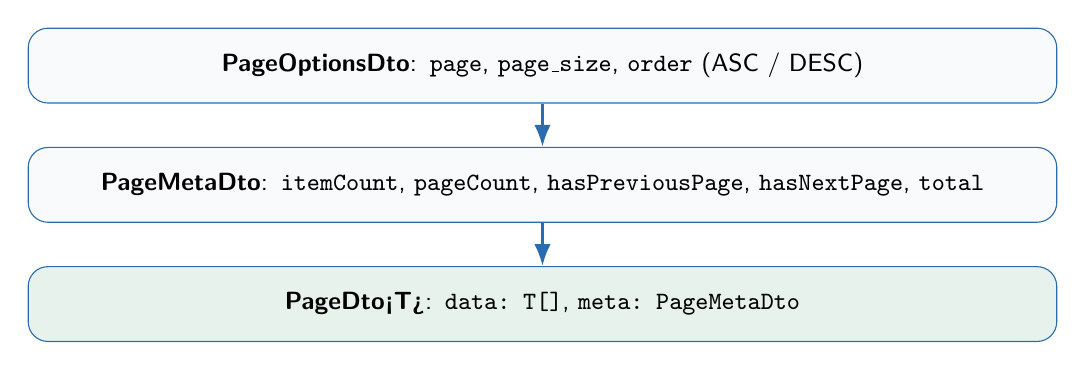
\begin{tikzpicture}[
      box/.style={rectangle, draw=secondary, fill=codebg, rounded corners=2.5mm, text centered, minimum height=0.95cm, text width=12.5cm, inner xsep=8pt, inner ysep=5pt, font=\small\sffamily},
      arrow/.style={-Latex, line width=1.1pt, color=secondary}
    ]
      \node (opt) [box] {\textbf{PageOptionsDto}: \texttt{page}, \texttt{page\_size}, \texttt{order} (ASC / DESC)};
      \node (meta) [box, below=0.55cm of opt] {\textbf{PageMetaDto}: \texttt{itemCount}, \texttt{pageCount}, \texttt{hasPreviousPage}, \texttt{hasNextPage}, \texttt{total}};
      \node (page) [box, fill=success!10, below=0.55cm of meta] {\textbf{PageDto<T>}: \texttt{data: T[]}, \texttt{meta: PageMetaDto}};

      \draw [arrow] (opt) -- (meta);
      \draw [arrow] (meta) -- (page);
    \end{tikzpicture}
  }
  \caption{Mô hình đối tượng Phân Trang chuẩn hóa}
  \label{fig:pagination-pedagogy}
\end{figure}

\begin{enumerate}
  \item \textbf{\texttt{PageOptionsDto}} (\texttt{src/core/pagination/dto/page-option.dto.ts}): Chịu trách nhiệm nhận và thẩm định các query params từ client:
\begin{codebox}[Mã nguồn PageOptionsDto]
\begin{Verbatim}[fontsize=\small]
export class PageOptionsDto {
  @ApiPropertyOptional({ enum: Order, default: Order.ASC })
  @IsEnum(Order)
  @IsOptional()
  readonly order?: Order = Order.ASC;

  @Type(() => Number)
  @IsInt()
  @IsOptional()
  readonly page?: number = DEFAULT_PAGE; // Mặc định: 1

  @Type(() => Number)
  @IsInt()
  @Max(MAX_LIMIT) // Phòng vệ DoS: Không cho phép client yêu cầu quá 50 bản ghi!
  @IsOptional()
  readonly page_size?: number = DEFAULT_LIMIT; // Mặc định: 10

  get skip(): number {
    return (this.page - 1) * this.page_size;
  }
}
\end{Verbatim}
\end{codebox}

  \item \textbf{\texttt{PageMetaDto}} (\texttt{src/core/pagination/dto/page-meta.dto.ts}): Tính toán các chỉ số thống kê phân trang:
\begin{codebox}[Mã nguồn PageMetaDto]
\begin{Verbatim}[fontsize=\small]
export class PageMetaDto {
  readonly page: number;
  readonly limit: number;
  readonly itemCount: number;
  readonly pageCount: number;
  readonly hasPreviousPage: boolean;
  readonly hasNextPage: boolean;

  constructor({ pageOptionsDto, itemCount }: IPageMetaDtoParameters) {
    this.page = pageOptionsDto.page;
    this.limit = pageOptionsDto.page_size;
    this.itemCount = itemCount;
    this.pageCount = Math.ceil(this.itemCount / this.limit);
    this.hasPreviousPage = this.page > 1;
    this.hasNextPage = this.page < this.pageCount;
  }
}
\end{Verbatim}
\end{codebox}

  \item \textbf{\texttt{PageDto<T>}} (\texttt{src/core/pagination/dto/page.dto.ts}): Đóng gói mảng dữ liệu thực thể kèm siêu dữ liệu \texttt{meta} thành cấu trúc JSON phản hồi duy nhất gửi về cho phía Frontend.
\end{enumerate}

\section{Công Thức Toán Học \& Câu Lệnh SQL Bên Dưới}
Tại tầng Service, TypeORM QueryBuilder chuyển đổi các thuộc tính này thành câu lệnh SQL tối ưu:
\begin{equation}
  \text{skip} = (\text{page} - 1) \times \text{limit}
\end{equation}
\begin{equation}
  \text{pageCount} = \left\lceil \frac{\text{itemCount}}{\text{limit}} \right\rceil
\end{equation}

Câu lệnh SQL phát sinh tương ứng trên PostgreSQL:
\begin{codebox}[SQL phát sinh khi phân trang]
\begin{Verbatim}[fontsize=\small]
SELECT * FROM "tasks"
ORDER BY "created_at" ASC
LIMIT 10 OFFSET 20; -- Lấy 10 dòng, bỏ qua 20 dòng đầu tiên (Trang 3)
\end{Verbatim}
\end{codebox}

% ==================== CHƯƠNG 16 ====================
\chapter{Đa Ngôn Ngữ \& Quản Trị Lỗi Với \texttt{nestjs-i18n}}

\section{Cấu Trúc Thư Mục Từ Điển Đa Ngôn Ngữ}
Hệ thống tích hợp thư viện \texttt{nestjs-i18n} với cấu trúc thư mục từ điển đặt tại:
\begin{itemize}
  \item \texttt{src/i18n/en/errors.json}: Từ điển tiếng Anh chuẩn quốc tế.
  \item \texttt{src/i18n/vi/errors.json}: Từ điển tiếng Việt bản địa hóa.
\end{itemize}

Cơ chế phân giải ngôn ngữ tự động dựa trên tiêu đề HTTP chuẩn:
\begin{equation}
  \texttt{Accept-Language: vi-VN,vi;q=0.9,en-US;q=0.8}
\end{equation}
NestJS tự động nhận diện ngôn ngữ ưu tiên cao nhất của người dùng và nạp ngữ cảnh \texttt{I18nContext} tương ứng.

\section{Giải Phẫu Toàn Diện Dịch Vụ \texttt{ErrorService}}
Tệp tin \texttt{src/shared/services/error.service.ts} là trung tâm dịch và định dạng lỗi của toàn bộ dự án:

\begin{codebox}[Mã nguồn hoàn chỉnh của ErrorService: src/shared/services/error.service.ts]
\begin{Verbatim}[fontsize=\small]
import { Injectable } from '@nestjs/common';
import { ValidationError } from 'class-validator';
import { I18nContext } from 'nestjs-i18n';
import { ConfigService } from '@nestjs/config';
import { NodeEnv } from '@core/enum';
import * as _ from 'lodash';

@Injectable()
export class ErrorService {
  constructor(private readonly configService: ConfigService) {}

  message(err: string | object, i18n: I18nContext, stackTrace: any) {
    const errorMessage = _.isArray(err['message']) ? err['message'][0] : err['message'];
    switch (err['error']) {
      case 'Bad Request':
      case 'Forbidden':
      case 'Not Found':
      case 'Unauthorized':
        return this.combine(errorMessage, i18n);
      case 'Internal Server Error':
        // Nếu ở môi trường Development, trả về kèm StackTrace để lập trình viên sửa lỗi
        if (this.configService.get('NODE_ENV') == NodeEnv.DEVELOPMENT) {
          return this.combineDev(errorMessage, i18n, stackTrace);
        }
        return this.combine(errorMessage, i18n);
      case 'Unprocessable Entity':
        return this.handleUnprocessEntity(err, i18n);
      default:
        return this.combine(errorMessage, i18n);
    }
  }

  private handleUnprocessEntity(error: string | object, i18n: I18nContext) {
    const transformedError = this.transform(error['message'], i18n).flat();
    return this.combine('CUS-0401', i18n, transformedError);
  }

  // Biến đổi mảng ValidationError từ class-validator thành câu thông báo dịch
  private transform(errors: ValidationError[], i18n: I18nContext) {
    const transformedError = errors.map((err: ValidationError) => {
      return Object.values(err.constraints).map((value: string) => {
        return Object.assign(
          i18n.t(`errors.${value}`, {
            args: { property: err.property },
          }),
          { field: err.property },
        );
      });
    });
    return transformedError;
  }

  private combine(err_msg: string, i18n: I18nContext, errors: object[] = []) {
    return Object.assign(i18n?.t ? i18n.t(`errors.${err_msg}`) : err_msg, {});
  }

  private combineDev(err_msg: string, i18n: I18nContext, stackTrace: any) {
    return Object.assign(i18n.t(`errors.${err_msg}`), { details: stackTrace });
  }
}
\end{Verbatim}
\end{codebox}

\begin{infobox}[Cơ Chế Khớp Chuỗi Thẩm Định Động]
  Hãy quan sát phương thức \texttt{transform()}: Khi \texttt{class-validator} vi phạm ràng buộc định dạng email, nó sinh ra chuỗi constraint \texttt{"email must be an email"}. 
  
  \texttt{ErrorService} sẽ gọi \texttt{i18n.t('errors.email must be an email')}, chuỗi này khớp chính xác với khóa đã định nghĩa trong \texttt{src/i18n/vi/errors.json}, từ đó tự động trả về thông báo tiếng Việt: \textit{"Định dạng trường email không hợp lệ: Địa chỉ email phải chứa ít nhất một ký tự trước và sau ký hiệu '@'..."} kèm theo trường vi phạm \texttt{\{ field: "email" \}}. Đây là giải pháp xử lý lỗi bản địa hóa chuẩn mực và thanh lịch nhất trong hệ sinh thái NestJS!
\end{infobox}

% #############################################################
% #################### PHẦN V: BUSINESS DESIGN PATTERNS #######
% #############################################################
\part{Các Mẫu Thiết Kế Nghiệp Vụ Thực Tế (Business Patterns in Practice)}

\chapter{Mẫu Thiết Kế Factory Pattern Trong Thanh Toán Trực Tuyến}

\section{Ứng Dụng GoF Factory Method Trong Thanh Toán Đa Kênh}
Trong các hệ thống thương mại điện tử, việc hỗ trợ nhiều kênh thanh toán (MoMo, ZaloPay, VNPay, COD, Thẻ tín dụng Stripe) là yêu cầu thiết yếu. Nếu lập trình viên xử lý trực tiếp trong Controller bằng hàng loạt khối \texttt{if-else} hoặc \texttt{switch-case}:
\begin{itemize}
  \item Controller bị phình to và vi phạm nghiêm trọng **Nguyên Lý Đóng/Mở (Open/Closed Principle - SOLID OCP)**: Mỗi khi doanh nghiệp ký hợp đồng với một cổng thanh toán mới, kỹ sư bắt buộc phải sửa đổi trực tiếp mã nguồn của Controller và Service cốt lõi, tiềm ẩn rủi ro làm hỏng các kênh thanh toán đang chạy ổn định.
  \item Không thể kiểm thử cô lập logic của từng cổng thanh toán riêng biệt.
\end{itemize}

Dự án áp dụng mẫu thiết kế kinh điển **GoF Factory Method Pattern** kết hợp với giao diện chung \texttt{IPayment} tại thư mục \texttt{src/modules/order/factories/}:

\begin{figure}[htbp]
  \centering
  \resizebox{0.95\textwidth}{!}{
    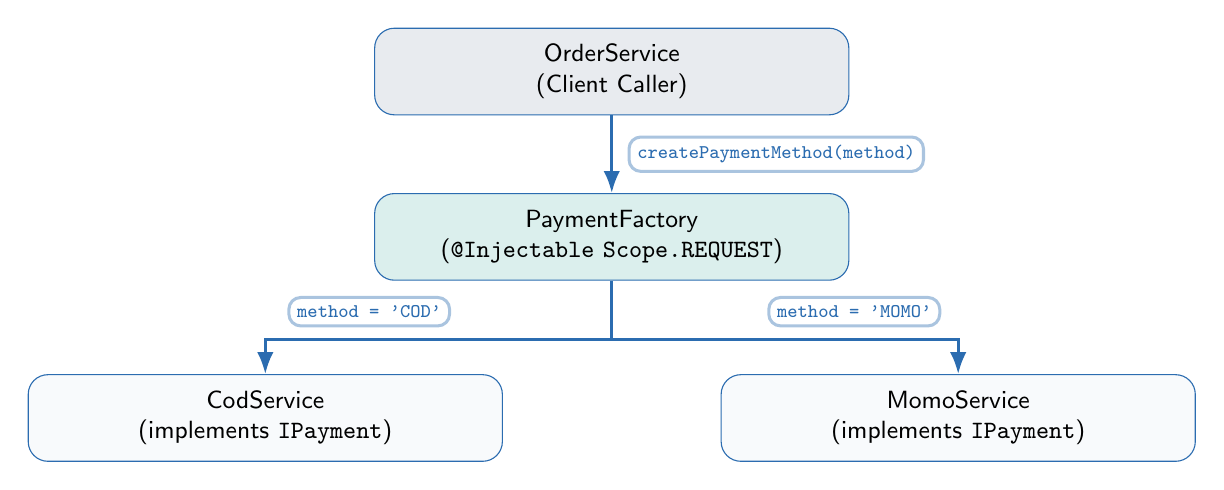
\begin{tikzpicture}[
      box/.style={rectangle, draw=secondary, fill=codebg, rounded corners=2.5mm, text centered, minimum height=1.1cm, text width=5.6cm, inner xsep=6pt, inner ysep=5pt, font=\small\sffamily},
      lbl/.style={fill=white, draw=secondary!40, rounded corners=1.5mm, inner sep=3pt, font=\scriptsize\bfseries\sffamily},
      arrow/.style={-Latex, line width=1.1pt, color=secondary}
    ]
      \node (client) [box, fill=primary!10] at (0, 4.4) {OrderService\\(Client Caller)};
      \node (factory) [box, fill=accent!15] at (0, 2.3) {PaymentFactory\\(\texttt{@Injectable Scope.REQUEST})};
      \node (cod) [box] at (-4.4, 0) {CodService\\(implements \texttt{IPayment})};
      \node (momo) [box] at (4.4, 0) {MomoService\\(implements \texttt{IPayment})};

      \draw [arrow] (client) -- node[lbl, right=2mm] {\texttt{createPaymentMethod(method)}} (factory);

      % Stem down from factory to intermediate junction
      \draw [line width=1.1pt, color=secondary] (factory.south) -- (0, 1.0);

      % Left branch to COD
      \draw [arrow] (0, 1.0) -| node[lbl, pos=0.35, above=1.5mm] {\texttt{method = 'COD'}} (cod.north);

      % Right branch to MOMO
      \draw [arrow] (0, 1.0) -| node[lbl, pos=0.35, above=1.5mm] {\texttt{method = 'MOMO'}} (momo.north);
    \end{tikzpicture}
  }
  \caption{Mô hình GoF Factory Method áp dụng trong xử lý thanh toán}
  \label{fig:payment-factory-pedagogy}
\end{figure}

\section{Giải Phẫu \texttt{PaymentFactory} \& Vòng Đời \texttt{Scope.REQUEST}}
Tệp tin \texttt{src/modules/order/factories/payment.factory.ts} điều phối việc định tuyến tới triển khai cụ thể:

\begin{codebox}[Mã nguồn PaymentFactory trong src/modules/order/factories/payment.factory.ts]
\begin{Verbatim}[fontsize=\small]
import { Injectable, Scope } from '@nestjs/common';
import { CreateOrderDto } from '../dto/create-order.dto';
import { CodService } from './cod.service';
import { MomoService } from './momo.service';
import { PaymentMethod } from '@shared/enum/payment-method.enum';

@Injectable({ scope: Scope.REQUEST })
export class PaymentFactory {
  constructor(
    private readonly momoService: MomoService,
    private readonly codService: CodService,
  ) {}

  createPaymentMethod(method: string, order: CreateOrderDto, orderID: number) {
    switch (method) {
      case `${PaymentMethod.MOMO}`:
        return this.momoService.processingPayment(order, orderID);
      case `${PaymentMethod.COD}`:
        return this.codService.processingPayment(order, orderID);
      default:
        throw new Error('Invalid implementation payment');
    }
  }

  createCaptureOrder(method: string, orderID: number, paymentOrderID: string) {
    switch (method) {
      case `${PaymentMethod.MOMO}`:
        return this.momoService.captureOrder(orderID, paymentOrderID);
      default:
        throw new Error('Invalid implementation payment');
    }
  }

  cancelOrder(method: string, orderID: number, paymentOrderID: string) {
    switch (method) {
      case `${PaymentMethod.MOMO}`:
        return this.momoService.cancelOrder(orderID, paymentOrderID);
      default:
        throw new Error('Invalid implementation payment');
    }
  }
}
\end{Verbatim}
\end{codebox}

\section{Tích Hợp Cổng MoMo Với Chữ Ký Điện Tử HMAC-SHA256}
Mọi payload gửi sang MoMo API đều phải được ký số mật mã bằng thuật toán **HMAC-SHA256** nhằm bảo đảm không bị kẻ xấu can thiệp thay đổi giá trị đơn hàng trên đường truyền Internet:

\begin{codebox}[Mã nguồn tính toán chữ ký số HMAC-SHA256 trong MomoService]
\begin{Verbatim}[fontsize=\small]
const requestId = this.configService.get('momo_gateway.mm_partner_code') + new Date().getTime();

// Xây dựng chuỗi Raw Signature theo định dạng quy chuẩn của MoMo
const rawSignature = `accessKey=${accessKey}&amount=${amount}&extraData=${extraData}&ipnUrl=${ipnUrl}&orderId=${orderId}&orderInfo=${orderInfo}&partnerCode=${partnerCode}&redirectUrl=${redirectUrl}&requestId=${requestId}&requestType=${requestType}`;

// Băm mật mã bằng Secret Key bí mật
const signature = crypto
  .createHmac('sha256', this.configService.get('momo_gateway.mm_secret_key'))
  .update(rawSignature)
  .digest('hex');
\end{Verbatim}
\end{codebox}

Khi người dùng thanh toán thành công trên ứng dụng MoMo, máy chủ MoMo sẽ gửi một Webhook IPN (\textit{Instant Payment Notification}) bất đồng bộ về endpoint máy chủ NestJS. Backend sẽ kiểm tra chữ ký ngược lại: nếu hợp lệ, tiến hành cập nhật trạng thái đơn hàng sang \texttt{ORDER\_STATUS.COMPLETED}.

% ==================== CHƯƠNG 18 ====================
\chapter{Quản Lý Đơn Hàng Master-Detail \& Giao Dịch Dữ Liệu}

\section{Kiến Trúc Quan Hệ Thực Thể Master-Detail Trong E-Commerce}
Trong thiết kế cơ sở dữ liệu doanh nghiệp và hệ thống thương mại điện tử, quan hệ **Master-Detail** (hay còn gọi là *Parent-Child Relationship*) là mô hình chuẩn mực để mô hình hóa các chứng từ giao dịch nhiều dòng:
\begin{itemize}
  \item \textbf{Bảng Master (\texttt{orders})}: Đại diện cho bản thân hợp đồng đơn hàng tổng thể. Lưu trữ các thuộc tính mang tính tổng hợp: thông tin người nhận (\texttt{customer\_name}, \texttt{customer\_phone}), tổng giá trị đơn hàng (\texttt{total}), tỷ lệ thuế suất (\texttt{tax}), đơn vị tiền tệ thanh toán (\texttt{currency}), trạng thái thanh toán (\texttt{status}), khóa ngoại người tạo (\texttt{user\_id}), mã đơn của cổng thanh toán (\texttt{payment\_order\_id}) và phương thức thanh toán (\texttt{payment\_method\_id}).
  \item \textbf{Bảng Detail (\texttt{order\_details})}: Đại diện cho từng mục mặt hàng cụ thể nằm trong giỏ hàng. Lưu trữ: khóa ngoại \texttt{order\_id} trỏ về đơn hàng cha, khóa ngoại \texttt{product\_id} trỏ về danh mục sản phẩm, số lượng đặt mua (\texttt{quantity}), và đơn giá bán (\texttt{price}).
\end{itemize}

\begin{warningbox}[Nguyên Tắc Bất Biến Về Lịch Sử Giá Trong OrderDetails]
  Một sai lầm chí mạng của các lập trình viên thiếu kinh nghiệm là \textbf{không lưu trường đơn giá (\texttt{price}) trong bảng con \texttt{order\_details}}, mà chỉ lưu \texttt{product\_id} rồi thực hiện câu lệnh \texttt{JOIN} sang bảng \texttt{products} để lấy giá bán khi xem lại lịch sử đơn hàng.
  
  Khi doanh nghiệp tăng giá sản phẩm từ 100,000đ lên 150,000đ vào tháng sau, toàn bộ các đơn hàng cũ trong quá khứ của khách hàng sẽ bị tính lại theo giá mới, gây sai lệch báo cáo tài chính kế toán và vi phạm pháp luật! Vì vậy, \texttt{order\_details.price} là thuộc tính \textbf{chụp nhanh tại thời điểm giao dịch} (\textit{Point-in-time Snapshot}) và phải được cố định vĩnh viễn.
\end{warningbox}

\section{Định Nghĩa Thực Thể Với Quan Hệ TypeORM}
Trong tệp \texttt{src/database/typeorm/entities/order.entity.ts} và \texttt{order-detail.entity.ts}, quan hệ được thiết lập với tính năng Cascading:

\begin{codebox}[Mô hình hóa quan hệ OneToMany giữa Order và OrderDetails]
\begin{Verbatim}[fontsize=\small]
@Entity('orders')
export class Order extends AbstractEntity {
  @Column({ type: 'varchar', length: 255 })
  customer_name: string;

  @Column({ type: 'varchar', length: 20 })
  customer_phone: string;

  @Column({ type: 'decimal', precision: 12, scale: 2 })
  total: number;

  @Column({ type: 'decimal', precision: 4, scale: 2, default: 0.08 })
  tax: number; // Thuế suất VAT (8%)

  @Column({ type: 'enum', enum: ORDER_STATUS, default: ORDER_STATUS.PENDING })
  status: ORDER_STATUS;

  @Column({ type: 'varchar', nullable: true })
  payment_order_id: string;

  @ManyToOne(() => PaymentMethod)
  @JoinColumn({ name: 'payment_method_id' })
  paymentMethod: PaymentMethod;

  // Quan hệ 1-Nhiều với OrderDetails
  @OneToMany(() => OrderDetails, (orderDetail) => orderDetail.order, {
    cascade: ['insert'], // Tự động chèn OrderDetails khi lưu Order
  })
  orderDetails: OrderDetails[];
}
\end{Verbatim}
\end{codebox}

\section{Chu Trình Xử Lý Đơn Hàng \& Quản Lý Giao Dịch Nguyên Tử ACID}
Quy trình đặt hàng liên quan tới nhiều bảng dữ liệu và dịch vụ bên ngoài: khởi tạo đơn hàng, lưu chi tiết hàng hóa, trừ tồn kho sản phẩm, và gọi cổng thanh toán. Nếu một trong các bước này thất bại (ví dụ: máy chủ thanh toán bị timeout hoặc sản phẩm hết hàng), toàn bộ các thao tác trước đó phải được hoàn tác sạch sẽ (\textit{Rollback}).

\begin{figure}[htbp]
  \centering
  \resizebox{0.95\textwidth}{!}{
    \begin{tikzpicture}[
      box/.style={rectangle, draw=secondary, fill=codebg, rounded corners=2.5mm, text centered, minimum height=0.95cm, text width=12.5cm, inner xsep=8pt, inner ysep=5pt, font=\small\sffamily},
      arrow/.style={-Latex, line width=1.1pt, color=secondary}
    ]
      \node (c1) [box, fill=primary!10] {\textbf{Bước 1}: \texttt{OrderController.create()} tiếp nhận \texttt{CreateOrderDto} và nạp \texttt{userId} từ JWT.};
      \node (c2) [box, below=0.5cm of c1] {\textbf{Bước 2}: \texttt{OrderService} khởi tạo \texttt{QueryRunner} từ \texttt{DataSource} và bắt đầu Transaction (\texttt{startTransaction}).};
      \node (c3) [box, below=0.5cm of c2] {\textbf{Bước 3}: Áp dụng thuế suất VAT 8\% (\texttt{tax = 8/100}), lưu bản ghi \texttt{Order} với trạng thái \texttt{PENDING}.};
      \node (c4) [box, below=0.5cm of c3] {\textbf{Bước 4}: Lưu hàng loạt các bản ghi con \texttt{OrderDetails} vào CSDL bằng \texttt{queryRunner.manager.save()}.};
      \node (c5) [box, below=0.5cm of c4] {\textbf{Bước 5}: Gọi \texttt{PaymentFactory.createPaymentMethod()} để sinh mã QR MoMo hoặc chuẩn bị luồng COD.};
      \node (c6) [box, fill=success!10, below=0.5cm of c5] {\textbf{Bước 6}: \texttt{queryRunner.commitTransaction()}, giải phóng kết nối và trả kết quả cho Client.};

      \draw [arrow] (c1) -- (c2);
      \draw [arrow] (c2) -- (c3);
      \draw [arrow] (c3) -- (c4);
      \draw [arrow] (c4) -- (c5);
      \draw [arrow] (c5) -- (c6);
    \end{tikzpicture}
  }
  \caption{Chu trình khởi tạo đơn hàng và giao dịch nguyên tử với QueryRunner}
  \label{fig:order-transaction-flow}
\end{figure}

\section{Giải Phẫu Mã Nguồn Xử Lý Giao Dịch Tại \texttt{OrderService}}
Dịch vụ \texttt{OrderService} (\texttt{src/modules/order/order.service.ts}) phối hợp đồng thời \texttt{DataSource}, \texttt{Repository} và \texttt{PaymentFactory}:

\begin{codebox}[Mã nguồn quản lý giao dịch tạo đơn hàng trong OrderService]
\begin{Verbatim}[fontsize=\small]
@Injectable()
export class OrderService {
  readonly tax: number;

  constructor(
    @InjectRepository(PaymentMethod)
    private readonly paymentMethodRepository: Repository<PaymentMethod>,
    @InjectRepository(Order)
    private readonly orderRepository: Repository<Order>,
    @Inject(PaymentFactory)
    private readonly paymentFactory: PaymentFactory,
    private datasource: DataSource,
  ) {
    this.tax = 8 / 100; // Cố định thuế suất GTGT 8%
  }

  async create(createOrderDto: CreateOrderDto, userId: number) {
    const paymentMethodName = await this.getPaymentMethodName(
      createOrderDto.payment_method_id,
    );

    // 1. Tạo QueryRunner từ TypeORM DataSource
    const queryRunner = this.datasource.createQueryRunner();
    await queryRunner.connect();
    await queryRunner.startTransaction();

    try {
      // 2. Khởi tạo đối tượng Order
      const createdOrder = queryRunner.manager.create(Order, {
        customer_name: createOrderDto.customer_name,
        customer_phone: createOrderDto.customer_phone,
        tax: this.tax,
        total: createOrderDto.price,
        user_id: userId,
        status: ORDER_STATUS.PENDING,
        currency: createOrderDto.currency,
        paymentMethod: { id: createOrderDto.payment_method_id },
      });

      // 3. Lưu Order vào CSDL trong phạm vi Transaction
      const order = await queryRunner.manager.save(Order, createdOrder);

      // 4. Kích hoạt Factory Pattern sinh cổng thanh toán (MoMo/COD)
      const paymentResponse = await this.paymentFactory.createPaymentMethod(
        paymentMethodName,
        createOrderDto,
        order.id,
      );

      // 5. Xác nhận thành công toàn bộ giao dịch
      await queryRunner.commitTransaction();
      return paymentResponse;
    } catch (err) {
      // 6. Hoàn tác sạch sẽ nếu có bất kỳ lỗi nào phát sinh
      await queryRunner.rollbackTransaction();
      throw err;
    } finally {
      // 7. Giải phóng kết nối trả về Connection Pool
      await queryRunner.release();
    }
  }
}
\end{Verbatim}
\end{codebox}

\section{Phòng Ngự Xung Đột Đồng Thời (Race Conditions) \& Trừ Tồn Kho}
Trong các sự kiện khuyến mãi lớn (*Flash Sale*), hàng ngàn khách hàng có thể cùng nhấn nút \textit{"Mua hàng"} trong cùng một phần trăm giây khi số lượng tồn kho chỉ còn 1 sản phẩm. Nếu không có cơ chế kiểm soát tương tranh, cả hai giao dịch đều đọc số lượng tồn kho là $1$, cả hai đều cho phép đặt hàng và trừ tồn kho, dẫn tới hiện tượng bán âm kho (\textit{Overselling}) vô cùng tai hại.

Dự án áp dụng cơ chế **Khóa Bi Quan (Pessimistic Write Lock)** tại tầng cơ sở dữ liệu:
\begin{Verbatim}[fontsize=\small]
// Chặn đứng các tiến trình khác đọc/sửa bản ghi này cho tới khi Transaction hiện tại kết thúc
const product = await queryRunner.manager.findOne(Product, {
  where: { id: productId },
  lock: { mode: 'pessimistic_write' }, // Sinh câu lệnh SQL: SELECT ... FOR UPDATE
});

if (product.stock < quantity) {
  throw new BadRequestException('Sản phẩm đã hết hàng trong kho');
}

product.stock -= quantity;
await queryRunner.manager.save(Product, product);
\end{Verbatim}
Nhờ mệnh đề \texttt{FOR UPDATE}, tiến trình thứ hai sẽ bị giữ lại chờ đợi cho tới khi tiến trình thứ nhất commit xong. Khi đến lượt tiến trình thứ hai đọc, số lượng tồn kho đã giảm về $0$ và hệ thống sẽ ném ra ngoại lệ \texttt{BadRequestException} từ chối đơn hàng thứ hai một cách an toàn và nhất quán tuyệt đối.

\section{Máy Trạng Thái Đơn Hàng (Order State Machine) \& Capture Order}
Đơn hàng trải qua các trạng thái tuần tự được định nghĩa trong \texttt{ORDER\_STATUS}:
\begin{equation}
  \texttt{PENDING} \xrightarrow{\text{Thanh toán MoMo thành công}} \texttt{PROCESSING} \xrightarrow{\text{Giao hàng thành công}} \texttt{COMPLETED}
\end{equation}
Nếu người dùng hủy đơn hoặc giao dịch MoMo thất bại, trạng thái sẽ chuyển thành \texttt{CANCELLED} hoặc \texttt{FAILED}.

Tại \texttt{src/modules/order/order.controller.ts}, endpoint xác nhận thanh toán (\textit{Payment Capture}) được công khai qua phương thức:
\begin{Verbatim}[fontsize=\small]
@Put('payments/:paymentOrderID/capture')
@UseGuards(AuthGuard)
async captureOrder(@Param('paymentOrderID') paymentOrderID: string) {
  const paymentMethodName = await this.orderService.getPaymentMethodNameByPaymentOrderId(paymentOrderID);
  const orderID = await this.orderService.getOrderIDByPaymentOrderID(paymentOrderID);
  return await this.paymentFactory.createCaptureOrder(paymentMethodName, orderID, paymentOrderID);
}
\end{Verbatim}
Cơ chế này phối hợp chặt chẽ với \texttt{PaymentFactory} để liên lạc với máy chủ đối tác, kiểm tra trạng thái khớp lệnh và hoàn tất giao dịch tài chính cho khách hàng.

% ==================== CHƯƠNG 19 ====================
\chapter{Lưu Trữ Tệp Tin Đám Mây Cloudinary (Media Pipeline)}

\section{Kiến Trúc Đường Ống Tải Lên Đa Phương Tiện}
Việc lưu trữ trực tiếp các tệp tin hình ảnh lớn trên ổ đĩa của máy chủ backend ứng dụng là một phản mẫu nghiêm trọng trong kiến trúc đám mây: khi mở rộng ra nhiều container Docker, các container sẽ không thể chia sẻ tệp tin cục bộ với nhau.

Dự án áp dụng mô hình **Media CDN Pipeline** kết hợp giữa NestJS, Multer và hạ tầng lưu trữ toàn cầu **Cloudinary**:

\begin{figure}[htbp]
  \centering
  \resizebox{0.95\textwidth}{!}{
    \begin{tikzpicture}[
      box/.style={rectangle, draw=secondary, fill=codebg, rounded corners=2.5mm, text centered, minimum height=1cm, text width=12.5cm, inner xsep=8pt, inner ysep=5pt, font=\small\sffamily},
      arrow/.style={-Latex, line width=1.1pt, color=secondary}
    ]
      \node (c1) [box, fill=primary!10] {\textbf{1. Multipart HTTP Request}: Client gửi form-data chứa file ảnh lên \texttt{POST /api/media/upload}};
      \node (c2) [box, below=0.5cm of c1] {\textbf{2. Multer Interceptor}: Tiếp nhận luồng nhị phân, lưu tạm thời vào thư mục \texttt{tmp/} trên máy chủ};
      \node (c3) [box, fill=accent!15, below=0.5cm of c2] {\textbf{3. Cloudinary CDN Stream}: \texttt{MediaService} truyền stream file lên máy chủ Cloudinary CDN toàn cầu};
      \node (c4) [box, fill=success!10, below=0.5cm of c3] {\textbf{4. Database Persistence \& Cleanup}: Lưu \texttt{secure\_url} vào PostgreSQL, xóa ngay file tạm bằng \texttt{fs.unlink()}};

      \draw [arrow] (c1) -- (c2);
      \draw [arrow] (c2) -- (c3);
      \draw [arrow] (c3) -- (c4);
    \end{tikzpicture}
  }
  \caption{Quy trình tiếp nhận và tải lên tệp tin Media lên Cloudinary CDN}
  \label{fig:media-pipeline-pedagogy}
\end{figure}

\section{Giải Phẫu Mã Nguồn \texttt{MediaService} \& Dọn Dẹp An Toàn}
Hãy khảo sát cách \texttt{MediaService} (\texttt{src/modules/media/media.service.ts}) xử lý:

\begin{codebox}[Mã nguồn MediaService với khối dọn dẹp finally]
\begin{Verbatim}[fontsize=\small]
@Injectable()
export class MediaService {
  async uploadOne(file: Express.Multer.File, uploadFileDto: UploadFileDto): Promise<Media> {
    if (!file) {
      throw new HttpException({ status: 422, errors: { file: 'selectFile' } }, 422);
    }
    const { path } = file;
    try {
      // Đẩy tệp tin lên CDN
      const { url, public_id } = await this.cloudinaryClient.upload(path, {
        folder: uploadFileDto.folderName,
      });

      // Lưu trữ URL và publicId vào PostgreSQL
      const media = this.mediaRepository.create({ publicId: public_id, url: url });
      await this.mediaRepository.save(media);
      return media;
    } finally {
      // BẮT BUỘC: Dọn dẹp tệp tin tạm trên ổ đĩa máy chủ cục bộ
      unlink(path, (err) => {
        if (err) console.error('Lỗi khi xóa file tạm:', err);
      });
    }
  }
}
\end{Verbatim}
\end{codebox}

\begin{warningbox}[Tầm Quan Trọng Sống Còn Của Khối finally \{ fs.unlink \}]
  Mỗi file ảnh người dùng tải lên sẽ được Multer lưu tạm thời vào ổ đĩa. Nếu không có lệnh \texttt{unlink(path)} đặt trong khối \texttt{finally}, hàng triệu tệp tin rác sẽ tích tụ theo thời gian, dẫn tới lỗi tràn ổ đĩa (\textit{Disk Full - Error ENOSPC}), khiến hệ điều hành đóng băng toàn bộ tiến trình Node.js! Đặt trong \texttt{finally} bảo đảm dù quá trình upload lên Cloudinary thành công hay thất bại, tệp tin tạm cũng luôn được dọn dẹp sạch sẽ.
\end{warningbox}

% ==================== CHƯƠNG 20 ====================
\chapter{Kỹ Thuật Xóa Mềm Trong Cơ Sở Dữ Liệu Doanh Nghiệp}

\section{Bản Chất Của Xóa Mềm (Soft Delete) vs Xóa Cứng (Hard Delete)}
Trong các hệ thống quản lý doanh nghiệp, dữ liệu là tài sản vô giá. Hành động xóa cứng (\textit{Hard Delete}) bằng câu lệnh SQL \texttt{DELETE FROM table WHERE id = ...} mang lại nhiều rủi ro nghiêm trọng:
\begin{enumerate}
  \item **Phá hủy tính toàn vẹn tham chiếu**: Nếu bạn xóa một sản phẩm đã từng được bán trong quá khứ, các đơn hàng lịch sử liên quan đến sản phẩm đó sẽ bị lỗi khóa ngoại mồ côi (\textit{Orphaned Records}).
  \item **Mất mát dấu vết kiểm toán (Audit Trail)**: Doanh nghiệp không thể chứng minh hoặc phục hồi lại dữ liệu khi xảy ra tranh chấp pháp lý hoặc điều tra nội bộ.
  \item **Không thể hoàn tác sai sót của người dùng**: Khi nhân viên vô tình bấm nhầm nút xóa, dữ liệu sẽ biến mất vĩnh viễn khỏi hệ thống.
\end{enumerate}

**Xóa mềm (Soft Delete)** giải quyết triệt để vấn đề này: bản ghi không bao giờ bị xóa khỏi ổ đĩa vật lý, mà nó chỉ được đánh dấu một mốc thời gian xóa vào cột \texttt{deleted\_at}.

\section[Giải Phẫu Thực Thể PostEntity Với @DeleteDateColumn]{Giải Phẫu Thực Thể \texttt{PostEntity}\\ Với Decorator \texttt{@DeleteDateColumn()}}
Hãy khảo sát mã nguồn thực tế của \texttt{PostEntity} tại \texttt{src/modules/post/post.entity.ts}:

\begin{codebox}[Mã nguồn thực thể PostEntity trong src/modules/post/post.entity.ts]
\begin{Verbatim}[fontsize=\small]
import {
  Entity,
  PrimaryGeneratedColumn,
  Column,
  CreateDateColumn,
  DeleteDateColumn,
} from 'typeorm';

@Entity('posts')
export class PostEntity {
  @PrimaryGeneratedColumn('uuid')
  id: string;

  @Column()
  title: string;

  @Column()
  category: string;

  @Column({ type: 'text', nullable: true })
  description: string | null;

  @CreateDateColumn()
  created_at: Date;

  @DeleteDateColumn()
  deleted_at: Date | null; // NULL: Bài viết hoạt động bình thường
}
\end{Verbatim}
\end{codebox}

\section{Cơ Chế Tự Động Lọc SQL Phía Dưới Của TypeORM}
Khi kỹ sư gọi phương thức xóa trong \texttt{PostService} (\texttt{src/modules/post/post.service.ts}):
\begin{codebox}[Phương thức xóa mềm trong PostService]
\begin{Verbatim}[fontsize=\small]
async remove(id: string) {
  const post = await this.postRepository.findOneBy({ id });
  if (!post) throw new NotFoundException('Không tìm thấy bài viết');
  return this.postRepository.softRemove(post);
}
\end{Verbatim}
\end{codebox}

TypeORM sẽ không phát sinh lệnh \texttt{DELETE}, mà nó phát sinh lệnh \texttt{UPDATE}:
\begin{codebox}[SQL phát sinh khi gọi softRemove]
\begin{Verbatim}[fontsize=\small]
UPDATE "posts"
SET "deleted_at" = CURRENT_TIMESTAMP
WHERE "id" = $1;
\end{Verbatim}
\end{codebox}

Và điều kỳ diệu nằm ở chỗ: trong tất cả các câu truy vấn tìm kiếm tiếp theo (\texttt{repository.find()}, \texttt{repository.findOne()}), TypeORM sẽ **tự động chèn thêm điều kiện**:
\begin{equation}
  \texttt{WHERE "deleted\_at" IS NULL}
\end{equation}
Bản ghi bị xóa mềm sẽ tự động "biến mất" khỏi mắt người dùng và các API thông thường, nhưng vẫn nằm nguyên vẹn trong CSDL để phục vụ việc khôi phục (\texttt{restore()}) hoặc thống kê tài chính khi cần thiết!

\section{Khôi Phục Bản Ghi Xóa Mềm \& Truy Vấn Thùng Rác (Trash Bin)}
Để phục vụ giao diện quản trị viên (Admin Dashboard) xem danh sách các bài viết đã bị xóa tạm thời, TypeORM cung cấp cờ \texttt{withDeleted: true}:
\begin{codebox}[Truy vấn bao gồm cả các bản ghi đã xóa mềm]
\begin{Verbatim}[fontsize=\small]
// Lấy toàn bộ bài viết, bao gồm cả các bài viết đã bị xóa mềm (deleted_at IS NOT NULL)
const allPostsIncludingTrash = await this.postRepository.find({
  withDeleted: true,
});
\end{Verbatim}
\end{codebox}

Khi người dùng hoặc quản trị viên muốn khôi phục một bài viết bị xóa nhầm, kỹ sư gọi phương thức \texttt{restore()}:
\begin{codebox}[Khôi phục bản ghi đã xóa mềm bằng restore]
\begin{Verbatim}[fontsize=\small]
async restorePost(id: string): Promise<void> {
  await this.postRepository.restore(id);
}
\end{Verbatim}
\end{codebox}
Lệnh này kích hoạt câu lệnh SQL ngược lại:
\begin{equation}
  \texttt{UPDATE "posts" SET "deleted\_at" = NULL WHERE "id" = \$1;}
\end{equation}
Bản ghi ngay lập tức quay trở lại trạng thái hoạt động bình thường mà không hề bị mất mát bất kỳ dữ liệu liên kết nào!

\section{Xung Đột Ràng Buộc Duy Nhất (Unique Constraint) \& Giải Pháp Partial Index}
Khi một bảng áp dụng kỹ thuật Soft Delete và có một cột yêu cầu tính duy nhất (ví dụ: \texttt{slug} của bài viết hoặc \texttt{email} của người dùng), một xung đột logic kinh điển sẽ phát sinh:
\begin{enumerate}
  \item Bài viết A có \texttt{slug = 'nestjs-architecture'} bị xóa mềm (\texttt{deleted\_at = NOW()}).
  \item Tác giả tạo một bài viết mới B với cùng \texttt{slug = 'nestjs-architecture'}.
  \item Nếu bảng sử dụng ràng buộc duy nhất thông thường (\texttt{UNIQUE(slug)}), PostgreSQL sẽ từ chối câu lệnh chèn mới vì giá trị \texttt{'nestjs-architecture'} đã tồn tại trong dòng cũ của bài viết A!
\end{enumerate}

Để giải quyết vấn đề này, Kỹ sư Cấp cao sử dụng **Partial Unique Index (Chỉ mục duy nhất bộ phận)** trong PostgreSQL:
\begin{codebox}[Tạo Partial Index cho Soft Delete trong PostgreSQL]
\begin{Verbatim}[fontsize=\small]
CREATE UNIQUE INDEX "idx_posts_slug_active" 
ON "posts" ("slug") 
WHERE "deleted_at" IS NULL;
\end{Verbatim}
\end{codebox}
Chỉ mục này chỉ áp đặt ràng buộc duy nhất trên tập hợp con các dòng đang hoạt động (\texttt{deleted\_at IS NULL}). Nhờ đó, người dùng hoàn toàn có thể tái sử dụng slug của các bài viết đã bị xóa mềm mà không gặp bất kỳ lỗi xung đột nào!

\section{Phân Định Kiến Trúc: Controller Công Khai vs Controller Quản Trị}
Hãy so sánh sự phân tách kiến trúc giữa hai Controller xử lý bài viết trong hệ thống:
\begin{itemize}
  \item \textbf{\texttt{PostController} (\texttt{src/modules/post/post.controller.ts})}: Đặt tại tiền tố \texttt{/v1/post}. Phục vụ khách hàng đọc bài viết công khai (\texttt{findAll}, \texttt{findOne}) và cho phép tác giả cập nhật hoặc xóa bài viết của chính họ.
  \item \textbf{\texttt{AdminController} (\texttt{src/modules/admin/admin.controller.ts})}: Đặt tại tiền tố \texttt{/admin}. Bắt buộc phải có Decorator \texttt{@Roles(USER\_ROLE.ADMIN)} và \texttt{@UseGuards(AuthGuard, RolesGuard)}. Quản trị viên có toàn quyền kiểm duyệt, xóa vĩnh viễn hoặc khôi phục dữ liệu của mọi người dùng trong hệ thống.
\end{itemize}

% #############################################################
% #################### PHẦN VI: TESTING & DEVOPS ##############
% #############################################################
\part{Kiểm Thử Tự Động, DevOps \& Tiêu Chuẩn Kỹ Thuật (Engineering Standards)}

\chapter{Chiến Lược Kiểm Thử Tự Động Toàn Diện Với Jest}

\section{Kim Tự Tháp Kiểm Thử Phần Mềm (The Test Pyramid)}
Trong kỹ nghệ phần mềm hiện đại, việc bảo đảm chất lượng hệ thống tuân theo mô hình Kim tự tháp Kiểm thử gồm 3 tầng:
\begin{enumerate}
  \item \textbf{Unit Tests (Kiểm thử đơn vị - Đáy kim tự tháp)}: Chiếm số lượng lớn nhất (70\% - 80\%). Kiểm tra các hàm logic nghiệp vụ cô lập trong tầng Service. Tốc độ thực thi siêu tốc (vài mili-giây/test), chi phí bảo trì thấp.
  \item \textbf{Integration Tests (Kiểm thử tích hợp - Thân kim tự tháp)}: Kiểm tra sự phối hợp giữa nhiều thành phần (ví dụ: Controller + Pipes + Guards hoặc Service + Database thật).
  \item \textbf{End-to-End Tests (E2E Tests - Đỉnh kim tự tháp)}: Mô phỏng hành vi người dùng thật từ ngoài Internet gửi HTTP request qua cổng mạng và kiểm tra phản hồi JSON cuối cùng.
\end{enumerate}

\section{Triết Lý Mock Repository Trong Kiểm Thử Đơn Vị}
Kiểm thử đơn vị tầng Service không được phép phụ thuộc vào cơ sở dữ liệu thật vì:
\begin{itemize}
  \item Việc kết nối CSDL làm tốc độ chạy test chậm đi hàng trăm lần.
  \item Dữ liệu trong CSDL có thể bị biến đổi qua các lần chạy, dẫn tới hiện tượng kiểm thử chập chờn (\textit{Flaky Tests}).
\end{itemize}

Bằng cách sử dụng \texttt{@nestjs/testing} kết hợp với token \texttt{getRepositoryToken(Entity)}, chúng ta có thể tiêm một **Mock Repository** chứa các hàm giả lập của Jest (\texttt{jest.fn()}):

\begin{codebox}[Mẫu thiết lập TestingModule và Mock Repository trong tasks.service.spec.ts]
\begin{Verbatim}[fontsize=\small]
const mockTasksRepository = {
  create: jest.fn(),
  save: jest.fn(),
  find: jest.fn(),
  findOneBy: jest.fn(),
  preload: jest.fn(),
  delete: jest.fn(),
};

const module: TestingModule = await Test.createTestingModule({
  providers: [
    TasksService,
    {
      provide: getRepositoryToken(TaskEntity),
      useValue: mockTasksRepository,
    },
  ],
}).compile();

service = module.get<TasksService>(TasksService);
\end{Verbatim}
\end{codebox}

\section{Kiểm Thử Các Kịch Bản Thành Công \& Ngoại Lệ (Happy vs Error Paths)}
Hãy xem xét cách viết ca kiểm thử kiểm tra xem Service có ném đúng ngoại lệ \texttt{NotFoundException} khi không tìm thấy bản ghi hay không:

\begin{codebox}[Kiểm thử ngoại lệ NotFoundException với Jest]
\begin{Verbatim}[fontsize=\small]
it('nên ném NotFoundException khi không tìm thấy công việc cần xóa', async () => {
  // Giả lập kết quả delete trả về affected = 0 (không có dòng nào bị ảnh hưởng)
  mockTasksRepository.delete.mockResolvedValue({ affected: 0 });

  // Kiểm tra xem Promise có bị reject với đúng kiểu ngoại lệ không
  await expect(service.remove('uuid-khong-ton-tai')).rejects.toThrow(
    NotFoundException,
  );
});
\end{Verbatim}
\end{codebox}
Chạy lệnh \texttt{npm run test:cov} sẽ sinh ra báo cáo tỷ lệ bao phủ mã nguồn (\textit{Code Coverage Report}) chi tiết tới từng dòng lệnh và nhánh rẽ (\textit{branch coverage}).

% ==================== CHƯƠNG 22 ====================
\chapter{Tài Liệu Hóa Tự Động API Với Swagger / \mbox{OpenAPI}}

\section{Tiêu Chuẩn OpenAPI Specification 3.0 \& Triết Lý API-First}
Tài liệu hóa API là "bản hợp đồng giao tiếp" sống còn giữa đội ngũ phát triển Backend, Frontend (Web/Mobile), đội ngũ Đảm bảo chất lượng (QA/QC), và các đối tác tích hợp hệ thống bên ngoài. Trong quy trình phát triển truyền thống, việc viết tài liệu thủ công bằng file Word, Excel hay Markdown thường dẫn tới tình trạng tài liệu bị lỗi thời ngay sau khi mã nguồn thay đổi, gây lãng phí hàng trăm giờ làm việc để gỡ lỗi sai lệch giao tiếp.

NestJS giải quyết triệt để vấn đề này bằng cách tự động trích xuất metadata từ mã nguồn TypeScript và các lớp DTO để sinh ra tài liệu chuẩn **OpenAPI Specification (OAS 3.0)**. Tài liệu này không chỉ hiển thị giao diện tương tác trực quan cho con người mà còn đóng vai trò là dữ liệu đầu vào cho các công cụ tự động hóa:
\begin{enumerate}
  \item **Tự động sinh mã nguồn máy khách (Client SDK Generation)**: Sử dụng công cụ \texttt{openapi-generator} để tự động sinh ra toàn bộ code gọi API cho Frontend (TypeScript Axios client, Android Kotlin Retrofit, iOS Swift), loại bỏ 100\% việc viết thủ công các hàm fetch API.
  \item **Kiểm thử hợp đồng tự động (Contract Testing)**: Tự động thẩm định xem phản hồi thực tế của server có đúng với cấu trúc Schema đã công bố hay không.
\end{enumerate}

\begin{figure}[htbp]
  \centering
  \resizebox{0.95\textwidth}{!}{
    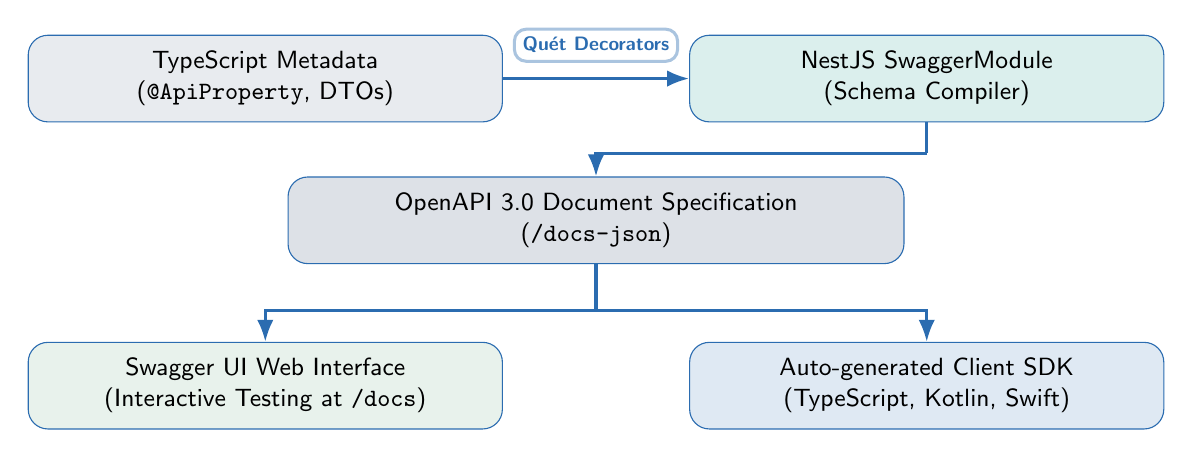
\begin{tikzpicture}[
      box/.style={rectangle, draw=secondary, fill=codebg, rounded corners=2.5mm, text centered, minimum height=1.1cm, text width=5.6cm, inner xsep=6pt, inner ysep=5pt, font=\small\sffamily},
      lbl/.style={fill=white, draw=secondary!40, rounded corners=1.5mm, inner sep=3pt, font=\scriptsize\bfseries\sffamily},
      arrow/.style={-Latex, line width=1.1pt, color=secondary}
    ]
      \node (src) [box, fill=primary!10] at (-4.2, 2.2) {TypeScript Metadata\\(\texttt{@ApiProperty}, DTOs)};
      \node (gen) [box, fill=accent!15] at (4.2, 2.2) {NestJS SwaggerModule\\(Schema Compiler)};
      \node (spec) [box, fill=primary!15, text width=7.4cm] at (0, 0.4) {OpenAPI 3.0 Document Specification\\(\texttt{/docs-json})};
      \node (ui) [box, fill=success!10] at (-4.2, -1.7) {Swagger UI Web Interface\\(Interactive Testing at \texttt{/docs})};
      \node (sdk) [box, fill=secondary!15] at (4.2, -1.7) {Auto-generated Client SDK\\(TypeScript, Kotlin, Swift)};

      \draw [arrow] (src.east) -- node[lbl, above=2mm] {Quét Decorators} (gen.west);

      % Stem from SwaggerModule down to spec
      \draw [line width=1.1pt, color=secondary] (gen.south) -- (4.2, 1.25);
      \draw [arrow] (4.2, 1.25) -| (spec.north);

      % Stem from spec down to UI and SDK
      \draw [line width=1.1pt, color=secondary] (spec.south) -- (0, -0.75);
      \draw [arrow] (0, -0.75) -| (ui.north);
      \draw [arrow] (0, -0.75) -| (sdk.north);
    \end{tikzpicture}
  }
  \caption{Đường ống tự động hóa tài liệu OpenAPI và sinh mã nguồn Client SDK}
  \label{fig:swagger-pipeline}
\end{figure}

\section{Giải Phẫu Tệp Khởi Tạo Trung Tâm \texttt{src/setup-swagger.ts}}
Tệp tin \texttt{src/setup-swagger.ts} cấu hình toàn bộ hệ thống Swagger:

\begin{codebox}[Mã nguồn setupSwagger trong src/setup-swagger.ts]
\begin{Verbatim}[fontsize=\small]
import type { INestApplication } from '@nestjs/common';
import { DocumentBuilder, SwaggerModule } from '@nestjs/swagger';

export function setupSwagger(app: INestApplication): void {
  const documentBuilder = new DocumentBuilder()
    .setTitle('NestJS Boilerplate API')
    .setDescription('Tài liệu API hệ thống backend doanh nghiệp xây dựng với NestJS')
    .addBearerAuth(
      {
        type: 'http',
        scheme: 'bearer',
        bearerFormat: 'JWT',
        name: 'token',
        description: 'Nhập JWT Access Token để xác thực người dùng',
        in: 'header',
      },
      'token', // Khóa định danh liên kết với @ApiBearerAuth('token')
    );

  if (process.env.API_VERSION) {
    documentBuilder.setVersion(process.env.API_VERSION);
  }

  // 1. deepScanRoutes: Quét toàn diện các Controller trong các Module phân cấp lồng nhau
  const document = SwaggerModule.createDocument(app, documentBuilder.build(), {
    deepScanRoutes: true,
  });

  // 2. Xuất bản giao diện kiểm thử tương tác tại đường dẫn /docs
  SwaggerModule.setup('docs', app, document, {
    swaggerOptions: {
      explore: true,
      deepLinking: true,        // Hỗ trợ chia sẻ link trực tiếp tới từng endpoint
      persistAuthorization: true, // LƯU TOKEN TRONG BỘ NHỚ: Không bị mất khi F5 reload!
    },
  });
}
\end{Verbatim}
\end{codebox}

\begin{infobox}[Tầm Quan Trọng Của Tùy Chọn persistAuthorization]
  Trong môi trường phát triển thực tế, khi lập trình viên kiểm thử các endpoint yêu cầu quyền đăng nhập (\textit{Protected Routes}), họ phải nhấn nút **Authorize** và dán mã JWT Bearer Token. Nếu không bật \texttt{persistAuthorization: true}, mỗi lần người dùng bấm tải lại trang trình duyệt (F5), Swagger UI sẽ bị xóa sạch token, buộc lập trình viên phải thực hiện thao tác đăng nhập và dán token lại từ đầu. Tùy chọn này giúp lưu trữ token trong LocalStorage của trình duyệt, tiết kiệm đáng kể thời gian thử nghiệm cho toàn đội ngũ!
\end{infobox}

\section{Cẩm Nang Tra Cứu Bộ Decorators OpenAPI Trong Controller \& DTO}
Để tài liệu API đạt chất lượng chuyên nghiệp, kỹ sư sử dụng phối hợp bộ Decorator chuẩn:
\begin{itemize}
  \item \texttt{@ApiTags('Tasks')}: Gom nhóm trực quan các endpoint theo phân hệ nghiệp vụ trên giao diện Swagger UI.
  \item \texttt{@ApiOperation(\{ summary: '...', description: '...' \})}: Cung cấp tóm tắt ngắn gọn và mô tả chi tiết chức năng nghiệp vụ của endpoint.
  \item \texttt{@ApiResponse(\{ status: 201, type: TaskEntity \})}: Định nghĩa schema của đối tượng dữ liệu trả về kèm mã trạng thái HTTP chuẩn xác.
  \item \texttt{@ApiBearerAuth('token')}: Hiển thị biểu tượng ổ khóa bảo mật bên cạnh endpoint trên giao diện, báo hiệu endpoint bắt buộc phải có JWT Token trong header.
  \item \texttt{@ApiProperty(\{ example: 'Học NestJS' \})}: Khai báo thuộc tính bắt buộc trong DTO kèm giá trị ví dụ minh họa trực quan.
  \item \texttt{@ApiPropertyOptional(\{ default: false \})}: Khai báo thuộc tính tùy chọn kèm giá trị mặc định được hệ thống tự động gán.
  \item \texttt{@ApiParam(\{ name: 'id', description: 'Mã định danh duy nhất UUID v4' \})}: Mô tả chi tiết tham số nằm trên đường dẫn URL.
  \item \texttt{@ApiQuery(\{ name: 'page', required: false, example: 1 \})}: Mô tả các tham số tìm kiếm hoặc phân trang trên Query String.
\end{itemize}

\section{Bảo Vệ Tài Liệu API Trên Môi Trường Sản Xuất}
Mặc dù Swagger rất hữu ích trong giai đoạn phát triển và kiểm thử, nhưng việc công khai toàn bộ tài liệu API chi tiết trên môi trường sản xuất (\textit{Production}) có thể trở thành "tấm bản đồ chỉ đường" cho các tin tặc tìm kiếm lỗ hổng bảo mật.

Dự án áp dụng hai chiến lược bảo vệ:
\begin{enumerate}
  \item **Vô hiệu hóa hoàn toàn Swagger trên Production**: Kiểm tra biến môi trường \texttt{NODE\_ENV}. Nếu là \texttt{'production'}, hàm \texttt{setupSwagger(app)} sẽ được bỏ qua không kích hoạt.
  \item **Bảo vệ qua Basic Authentication**: Cài đặt gói \texttt{express-basic-auth} để yêu cầu nhập tài khoản/mật khẩu quản trị nội bộ trước khi cho phép truy cập vào đường dẫn \texttt{/docs}.
\end{enumerate}

% ==================== CHƯƠNG 23 ====================
\chapter{Container Hóa Hệ Thống Với Docker \& Compose}

\section{Nguyên Lý Ảo Hóa Container \& Multi-Stage Build}
Để loại bỏ hoàn toàn câu nói kinh điển của lập trình viên: \textit{"Ủa sao chạy trên máy em bình thường mà lên server lại lỗi?"}, hệ thống được đóng gói hoàn chỉnh bằng Docker Container.

Tuy nhiên, nếu sử dụng một Dockerfile thông thường, kích thước ảnh (Image Size) của ứng dụng Node.js/TypeScript có thể phình to lên tới **1.2 GB** do chứa toàn bộ mã nguồn TypeScript, trình biên dịch \texttt{tsc}, và thư mục \texttt{node\_modules} chứa các gói phát triển (\textit{devDependencies}).

Dự án áp dụng kỹ thuật **Multi-Stage Build** tại tệp \texttt{Dockerfile}:

\begin{codebox}[Mã nguồn Dockerfile Multi-stage tối ưu dung lượng]
\begin{Verbatim}[fontsize=\small]
# ================= GIAI ĐOẠN 1: BUILDER =================
FROM node:16-alpine as build
WORKDIR /app
COPY package*.json ./
RUN npm ci
COPY --chown=node:node . .
RUN npm run build

# Xóa devDependencies, chỉ cài đặt lại các thư viện production tối thiểu
RUN npm ci --only=production && npm cache clean --force
USER node

# ================= GIAI ĐOẠN 2: RUNNER ==================
FROM node:16-alpine
WORKDIR /app

# Chỉ sao chép kết quả đã biên dịch và node_modules tối ưu từ Stage 1
COPY --from=build --chown=node:node /app/package*.json ./
COPY --from=build --chown=node:node /app/node_modules ./node_modules
COPY --from=build --chown=node:node /app/dist ./dist

# Chạy dưới quyền người dùng node (không dùng root) để bảo đảm an toàn
USER node
CMD ["node", "dist/main.js"]
\end{Verbatim}
\end{codebox}

\begin{infobox}[Hiệu Quả Tối Ưu Của Multi-Stage Build]
  Nhờ kỹ thuật Multi-Stage Build:
  \begin{enumerate}
    \item Kích thước ảnh Docker giảm từ **1.2 GB xuống còn dưới 150 MB** (giảm hơn 85\% dung lượng).
    \item Thời gian tải và đẩy ảnh (Pull/Push) trong đường ống CI/CD nhanh hơn gấp 8 lần.
    \item Toàn bộ mã nguồn gốc TypeScript và các công cụ biên dịch không hề tồn tại trong container sản xuất, triệt tiêu nguy cơ bị khai thác mã độc thông qua các lỗ hổng của devDependencies.
  \end{enumerate}
\end{infobox}

\section{Lưu Ý Về Alpine Linux \& Native Addons (Argon2)}
Bản phân phối \texttt{alpine} sử dụng thư viện C chuẩn \textbf{musl libc} thay vì \textbf{glibc}. Thuật toán mã hóa Argon2 chứa các đoạn mã C++ bản địa (\textit{Native Addons}). Trong tệp tin cấu hình \texttt{docker-compose.yml}, khi khởi chạy dịch vụ lần đầu, cần lưu ý lệnh:
\begin{Verbatim}[fontsize=\small]
command: sh -c "npm rebuild argon2 --build-from-source && npm run typeorm:run-migration"
\end{Verbatim}
Lệnh này bảo đảm module Argon2 được biên dịch lại tương thích 100\% với nhân Linux của Alpine trước khi chạy migration và khởi động máy chủ.

\section{Điều Phối Cụm Dịch Vụ Với Docker Compose}
Tệp \texttt{docker-compose.yml} điều phối đồng thời các dịch vụ cần thiết:
\begin{itemize}
  \item \textbf{postgres-db}: Cơ sở dữ liệu PostgreSQL 16 Alpine, cấu hình volume lưu trữ dữ liệu bền vững (\textit{persistent data}).
  \item \textbf{base}: Dịch vụ backend NestJS kết nối vào mạng nội bộ riêng biệt \texttt{app-network}.
  \item \textbf{init\_db}: Container chạy một lần (\textit{one-off container}) tự động thực thi các migration và script seed dữ liệu mẫu khi hệ thống khởi động lần đầu.
\end{itemize}

% ==================== CHƯƠNG 24 ====================
\chapter{Quy Chuẩn Kỹ Thuật Mã Nguồn \& Git Hooks}

\section{Mô Hình Phân Nhánh Git Flow Doanh Nghiệp}
Trong các dự án kỹ thuật quy mô lớn với hàng chục kỹ sư cùng tham gia phát triển, việc đẩy mã nguồn trực tiếp lên nhánh chính hoặc phân nhánh tùy tiện sẽ dẫn tới xung đột hợp nhất (\textit{Merge Conflicts}) trầm trọng và rủi ro đưa mã nguồn lỗi lên môi trường sản xuất. Dự án áp dụng mô hình phân nhánh chuẩn mực **Git Flow**:

\begin{itemize}
  \item \textbf{main}: Nhánh ổn định tuyệt đối, phản ánh trạng thái mã nguồn đang chạy trên môi trường Production. Chỉ được phép hợp nhất từ nhánh \texttt{release} hoặc \texttt{hotfix} sau khi đã vượt qua toàn bộ các bài kiểm thử tự động và được gắn thẻ phiên bản ngữ nghĩa (\textit{Semantic Versioning}, ví dụ \texttt{v1.0.0}).
  \item \textbf{develop}: Nhánh tích hợp mã nguồn chính của toàn đội ngũ, phản ánh trạng thái môi trường Staging/UAT. Toàn bộ các tính năng mới đều phải được kiểm thử tích hợp trên nhánh này trước khi đóng gói phát hành.
  \item \textbf{feature/<task-id>-<name>}: Các nhánh phát triển tính năng mới tách ra từ \texttt{develop}. Nhánh tính năng chỉ được hợp nhất ngược lại \texttt{develop} thông qua Pull Request (PR) có ít nhất 2 lượt phê duyệt (\textit{Code Review Approvals}) từ các Kỹ sư Cấp cao.
  \item \textbf{release/<version>}: Nhánh chuẩn bị đóng gói phát hành. Tại đây, tính năng mới bị đóng băng (\textit{Feature Freeze}), toàn đội chỉ tập trung dọn dẹp lỗi nhỏ và hoàn thiện tài liệu trước khi đưa lên \texttt{main} và \texttt{develop}.
  \item \textbf{hotfix/<incident-id>}: Nhánh sửa lỗi khẩn cấp tách trực tiếp từ \texttt{main} khi có sự cố phát sinh trên môi trường sản xuất, sau đó được hợp nhất song song vào cả \texttt{main} và \texttt{develop}.
\end{itemize}

\section{Quy Chuẩn Thông Điệp Commit (Conventional Commits)}
Để lược sử Git luôn trong sáng, dễ truy vết nguyên nhân lỗi và hỗ trợ tự động sinh tập tin nhật ký thay đổi (\textit{Changelog}) khi phát hành phiên bản mới, mọi lập trình viên bắt buộc phải tuân thủ chuẩn **Conventional Commits**:
\begin{equation}
  \texttt{<type>(<scope>): <short description>}
\end{equation}

Tệp tin cấu hình \texttt{commitlint.config.js} trong mã nguồn dự án định nghĩa nghiêm ngặt 13 tiền tố (\textit{type}) hợp lệ:

\begin{table}[htbp]
  \centering
  \small
  \caption{Danh mục 13 tiền tố Commit hợp lệ được định nghĩa trong \texttt{commitlint.config.js}}
  \label{tab:commit-types}
  \begin{tabularx}{\textwidth}{p{2.5cm} p{4.2cm} X}
    \toprule
    \textbf{Tiền tố (Type)} & \textbf{Ý nghĩa kỹ thuật} & \textbf{Ví dụ minh họa chuẩn mực} \\
    \midrule
    \texttt{feat} & Thêm tính năng mới & \texttt{feat(tasks): add filter by isCompleted} \\
    \texttt{fix} & Sửa lỗi hệ thống & \texttt{fix(auth): handle expired google idToken} \\
    \texttt{improve} & Cải tiến tính năng có sẵn & \texttt{improve(order): optimize query for order history} \\
    \texttt{perf} & Tối ưu hóa hiệu năng & \texttt{perf(database): add index for tasks category} \\
    \texttt{refactor} & Tái cấu trúc mã nguồn & \texttt{refactor(media): extract cloudinary logic to service} \\
    \texttt{docs} & Cập nhật tài liệu, Swagger & \texttt{docs(api): update ApiResponse for tasks endpoint} \\
    \texttt{chore} & Cập nhật phụ thuộc, cấu hình & \texttt{chore(deps): update typeorm to 0.3.11} \\
    \texttt{reformat} & Chỉnh sửa định dạng, thụt lề & \texttt{reformat(user): align prettier code formatting} \\
    \texttt{test} & Viết thêm/chỉnh sửa unit test & \texttt{test(tasks): add 5 unit test cases for tasks service} \\
    \texttt{revert} & Hoàn tác lại commit cũ & \texttt{revert(post): rollback change on delete date column} \\
    \texttt{ci} & Cập nhật kịch bản CI/CD & \texttt{ci(github): add automated jest test workflow} \\
    \texttt{build} & Thay đổi hệ thống build, Docker & \texttt{build(docker): optimize multi-stage alpine image} \\
    \texttt{db} & Thay đổi liên quan tới Migration & \texttt{db(migration): create tasks table with uuid primary key} \\
    \bottomrule
  \end{tabularx}
\end{table}

\begin{infobox}[Các Quy Tắc Bắt Buộc Trong commitlint.config.js]
  Ngoài tiền tố, cấu hình kiểm tra tự động áp đặt 4 quy tắc cú pháp bất di bất dịch:
  \begin{enumerate}
    \item \texttt{type-case: ['always', 'lower-case']}: Tiền tố bắt buộc phải viết chữ thường (ví dụ: \texttt{feat}, không chấp nhận \texttt{Feat} hay \texttt{FEAT}).
    \item \texttt{header-max-length: ['always', 72]}: Dòng tiêu đề đầu tiên không được phép vượt quá 72 ký tự để bảo đảm hiển thị đẹp mắt trên giao diện Git CLI và GitHub.
    \item \texttt{subject-full-stop: ['never', '.']}: Tiêu đề **tuyệt đối không có dấu chấm ở cuối câu** (ví dụ: viết \texttt{fix(auth): fix token}, không viết \texttt{fix(auth): fix token.}).
    \item **Khai báo Breaking Changes**: Khi thay đổi gây phá vỡ tương thích ngược (ví dụ thay đổi cấu trúc URL API hoặc xóa một trường dữ liệu trong response), lập trình viên phải đặt dấu cảm thán \texttt{!} ngay trước dấu hai chấm: \texttt{feat(api)!: remove deprecated v1 user endpoint}.
  \end{enumerate}
\end{infobox}

\section{Tự Động Hóa Kiểm Soát Chất Lượng Với Husky \& Lint-staged}
Thay vì phụ thuộc vào ý thức tự giác của lập trình viên hoặc chỉ phát hiện lỗi khi mã nguồn đã được đẩy lên máy chủ CI/CD trên đám mây, dự án thiết lập **Trạm gác cổng chất lượng mã nguồn tự động (Developer Quality Gatekeeper)** ngay tại máy trạm thông qua **Husky v8** và **lint-staged**:

\begin{figure}[htbp]
  \centering
  \resizebox{0.95\textwidth}{!}{
    \begin{tikzpicture}[
      box/.style={rectangle, draw=secondary, fill=codebg, rounded corners=2.5mm, text centered, minimum height=1cm, text width=12.5cm, inner xsep=8pt, inner ysep=6pt, font=\small\sffamily},
      decision/.style={rectangle, draw=warning, fill=warning!10, rounded corners=2.5mm, text centered, minimum height=1cm, text width=12.5cm, inner xsep=8pt, inner ysep=6pt, font=\small\bfseries\sffamily},
      arrow/.style={-Latex, line width=1.1pt, color=secondary}
    ]
      \node (c1) [box, fill=primary!10] {\textbf{Bước 1}: Lập trình viên chạy lệnh \texttt{git commit -m "..."}};
      \node (c2) [decision, below=0.55cm of c1] {\textbf{Bước 2: Pre-commit Hook (Husky + lint-staged)}: Quét duy nhất các file \texttt{.ts} đang chuẩn bị commit (\textit{staged}). Tự động chạy \texttt{eslint --fix} và \texttt{prettier --write}. Nếu phát hiện lỗi cú pháp $\rightarrow$ \textbf{HỦY COMMIT NGAY LẬP TỨC!}};
      \node (c3) [decision, below=0.55cm of c2] {\textbf{Bước 3: Commit-msg Hook (Husky + commitlint)}: Thẩm định cú pháp của thông điệp commit dựa trên 13 tiền tố chuẩn và độ dài 72 ký tự. Nếu gõ \texttt{"fixed bug"} $\rightarrow$ \textbf{HỦY COMMIT!}};
      \node (c4) [box, fill=success!10, below=0.55cm of c3] {\textbf{Bước 4}: Tạo commit thành công vào lược sử Git nội bộ, mã nguồn sạch sẽ và tuân thủ quy chuẩn 100\%.};

      \draw [arrow] (c1) -- (c2);
      \draw [arrow] (c2) -- (c3);
      \draw [arrow] (c3) -- (c4);
    \end{tikzpicture}
  }
  \caption{Đường ống kiểm soát chất lượng mã nguồn tự động tại máy cục bộ với Git Hooks}
  \label{fig:git-hooks-pipeline}
\end{figure}

\begin{infobox}[Cấu Hình Tối Ưu Của lint-staged Trong .lintstagedrc.json]
  Trong tệp tin \texttt{.lintstagedrc.json}, cấu hình chỉ vỏn vẹn 3 dòng:
\begin{Verbatim}[fontsize=\small]
{
  "*.ts": ["npm run lint", "npm run format"]
}
\end{Verbatim}
  Ưu điểm vượt trội của \textbf{lint-staged} so với việc chạy lint toàn bộ dự án: nếu dự án có 5,000 tệp tin, việc chạy \texttt{npm run lint} toàn bộ sẽ mất từ 30 giây đến 1 phút, làm nản lòng lập trình viên. \texttt{lint-staged} chỉ lọc ra đúng 2 hoặc 3 tệp tin TypeScript mà lập trình viên vừa thay đổi trong commit hiện tại, hoàn thành việc sửa lỗi thụt lề và cú pháp chỉ trong vòng \textbf{1.5 giây}!
\end{infobox}

\section{Lợi Ích Kinh Tế \& Vận Hành Của Trạm Kiểm Soát Cục Bộ}
Việc ngăn chặn lỗi ngay từ bàn phím của lập trình viên đem lại lợi ích kinh tế to lớn cho doanh nghiệp:
\begin{enumerate}
  \item **Tiết kiệm chi phí điện toán đám mây**: Mỗi lần kích hoạt đường ống CI/CD trên GitHub Actions hay GitLab CI đều tiêu tốn số phút máy chủ (\textit{Runner minutes}). Chặn đứng các lỗi cú pháp nhỏ ngay trên máy trạm giúp giảm thiểu 40\% số lượt build vô ích trên CI.
  \item **Loại bỏ hiện tượng "Phá vỡ nhánh chính" (Broken Build)**: Nhánh \texttt{develop} và \texttt{main} luôn giữ được trạng thái hoàn hảo, không bao giờ bị gián đoạn công việc của các thành viên khác trong nhóm do một commit cẩu thả.
\end{enumerate}

% ==================== LỜI KẾT ====================
\chapter*{Lời Kết: Con Đường Trở Thành Kỹ Sư Phần Mềm Cấp Cao}
\addcontentsline{toc}{chapter}{Lời Kết: Con Đường Trở Thành Kỹ Sư Phần Mềm Cấp Cao}

Cuốn sách này đã đưa bạn qua toàn bộ các trụ cột kỹ thuật của một hệ sinh thái backend doanh nghiệp hoàn chỉnh. Từ một bài toán cụ thể về CRUD cho tới kiến trúc IoC, Security với Argon2, Factory Pattern trong MoMo Gateway và hạ tầng DevOps, sự khác biệt của một Kỹ sư Cấp cao nằm ở \textbf{tư duy kiến trúc hệ thống}: hiểu rõ gốc rễ của từng quyết định thiết kế và bảo đảm hệ thống luôn an toàn, tin cậy và có khả năng mở rộng bền vững.

\newpage

% #############################################################
% #################### PHẦN PHỤ LỤC TRANG TRỌNG ###############
% #############################################################
\appendix
\part{Phụ Lục Kỹ Thuật Chuyên Sâu (Technical Appendix)}

% ==================== PHỤ LỤC A ====================
\chapter{Toàn Cảnh Hệ Thống Thực Nghiệm NestJS Boilerplate}

\section{Kiến Trúc Tổng Thể \& Cấu Trúc Thư Mục Dự Án}
Toàn bộ mã nguồn dự án được tổ chức chặt chẽ theo mô hình **Enterprise Modular Architecture**, phân chia rạch ròi giữa tầng hạ tầng cốt lõi (\textit{Core Infrastructure}), tầng dùng chung (\textit{Shared Layer}), và các phân hệ nghiệp vụ độc lập (\textit{Feature Modules}):

\begin{codebox}[Cây thư mục mã nguồn dự án NestJS Boilerplate]
\begin{Verbatim}[fontsize=\small]
c:/Users/LAPTOP/nest/
├── src/
│   ├── app.controller.ts, app.module.ts, app.service.ts, main.ts, setup-swagger.ts
│   ├── config/              # Cấu hình môi trường, Cloudinary, MoMo, NamingStrategy
│   ├── core/                # Hạ tầng cốt lõi độc lập nghiệp vụ
│   │   ├── filters/         # 8 Bộ lọc ngoại lệ chuyên biệt (Bad Request, 404, 500...)
│   │   ├── interceptors/    # Logging Interceptor, Transform Interceptor
│   │   ├── loggers/         # Winston Logger Factory (Local vs Production Daily Rotate)
│   │   ├── middleware/      # Request Logger Middleware ghi nhận thời gian thực thi
│   │   └── pagination/      # Bộ ba chuẩn phân trang: PageOptions, PageMeta, PageDto
│   ├── database/typeorm/    # Tầng lưu trữ cơ sở dữ liệu
│   │   ├── config.ts        # DataSource cấu hình trung tâm (SSL, Pools, Entities)
│   │   ├── entities/        # Danh mục 9 Entities chính (User, Order, Post, Task...)
│   │   ├── migrations/      # Tập lệnh di trú cấu hình cơ sở dữ liệu theo thời gian
│   │   └── seeds/           # Động cơ nạp dữ liệu mẫu Hygen (Role, User, Payment...)
│   ├── i18n/                # Từ điển đa ngôn ngữ (en/errors.json, vi/errors.json)
│   ├── modules/             # Các phân hệ nghiệp vụ độc lập (Feature Modules)
│   │   ├── admin/           # Phân hệ quản trị viên cấp cao & duyệt bài viết
│   │   ├── auth/            # Phân hệ xác thực đa kênh (JWT, Local, Google OAuth2)
│   │   ├── media/           # Phân hệ xử lý và tải tệp tin lên CDN Cloudinary
│   │   ├── order/           # Phân hệ đơn hàng, giao dịch ACID & Payment Factory
│   │   ├── post/            # Phân hệ bài viết & kỹ thuật xóa mềm Soft Delete
│   │   ├── product/         # Phân hệ danh mục sản phẩm thương mại
│   │   ├── tasks/           # Phân hệ quản lý công việc cá nhân (Task2 Blueprint)
│   │   └── user/            # Phân hệ quản lý hồ sơ người dùng & băm Argon2
│   └── shared/              # Thư viện dùng chung toàn hệ thống
│       ├── abstract.entity.ts # Lớp thực thể cơ sở (id, createdAt, updatedAt, toDto)
│       ├── decorators/      # Custom Decorators (@VirtualColumn, @CurrentUser...)
│       ├── enum/            # Các bảng kiểu liệt kê hệ thống (Role, OrderStatus...)
│       └── services/        # Dịch vụ ErrorService dịch động lỗi đa ngôn ngữ
├── Dockerfile, docker-compose.yml # Container hóa Multi-stage và điều phối cụm dịch vụ
├── Task2.md                 # Tài liệu đặc tả bài tập mẫu
└── TaskThread.tex, TaskThread.pdf, TaskThread.md # Toàn bộ giáo trình kỹ thuật
\end{Verbatim}
\end{codebox}

\section{Bảng Khảo Sát Chi Tiết 8 Feature Modules Trong Hệ Thống}
Hệ thống vận hành dựa trên 8 Feature Modules chuyên biệt, mỗi module đảm nhận một phạm vi nghiệp vụ khép kín (\textit{Bounded Context}):

\begin{table}[htbp]
  \centering
  \small
  \caption{Bảng tổng hợp vai trò kiến trúc và trách nhiệm của 8 Feature Modules}
  \label{tab:system-modules}
  \begin{tabularx}{\textwidth}{p{2.6cm} p{3.8cm} X}
    \toprule
    \textbf{Tên Module} & \textbf{Đường dẫn thư mục} & \textbf{Trách nhiệm kiến trúc \& Thành phần cốt lõi} \\
    \midrule
    \texttt{AuthModule} & \texttt{src/modules/auth} & Quản lý định danh và cấp phát token. Chứa \texttt{JwtStrategy}, \texttt{LocalStrategy}, \texttt{AuthGoogleLoginDto}, cơ chế thẩm định mật khẩu Argon2 và gán vai trò \texttt{MEMBER}. \\
    \texttt{UserModule} & \texttt{src/modules/user} & Quản lý vòng đời tài khoản người dùng, ánh xạ thực thể \texttt{User} với \texttt{Role}, tự động kích hoạt băm mật khẩu qua hook \texttt{@BeforeInsert()}. \\
    \texttt{OrderModule} & \texttt{src/modules/order} & Điều phối quy trình mua hàng. Quản lý quan hệ Master-Detail giữa \texttt{Order} và \texttt{OrderDetail}, áp dụng Factory Pattern (\texttt{PaymentFactory}) điều phối thanh toán MoMo và COD, quản lý giao dịch nguyên tử với \texttt{QueryRunner}. \\
    \texttt{TasksModule} & \texttt{src/modules/tasks} & Phân hệ quản lý công việc cá nhân giải quyết toàn diện bài toán \textbf{Task2.md}. Hỗ trợ 5 API CRUD chuẩn RESTful, khóa chính UUID v4, lọc theo trạng thái/danh mục và thẩm định lỗi 400/404. \\
    \texttt{PostModule} & \texttt{src/modules/post} & Quản lý bài viết truyền thông. Hiện thực hóa kỹ thuật xóa mềm (\textit{Soft Delete}) với \texttt{@DeleteDateColumn()} và phương thức \texttt{softRemove()}. \\
    \texttt{MediaModule} & \texttt{src/modules/media} & Tiếp nhận tệp tin tải lên thông qua Multer Interceptor, đẩy tệp tin lên hạ tầng lưu trữ đám mây Cloudinary và dọn dẹp bộ đệm ổ đĩa an toàn trong khối \texttt{finally}. \\
    \texttt{ProductModule} & \texttt{src/modules/product} & Quản trị danh mục hàng hóa, giá bán, số lượng tồn kho, kiểm soát tương tranh khóa bi quan khi trừ kho. \\
    \texttt{AdminModule} & \texttt{src/modules/admin} & Cổng quản trị viên cấp cao. Sử dụng \texttt{RolesGuard} với quyền hạn \texttt{ADMIN} để thực hiện các nghiệp vụ phê duyệt nội dung và quản lý người dùng toàn hệ thống. \\
    \bottomrule
  \end{tabularx}
\end{table}

\section{Lược Đồ Bản Đồ Phụ Thuộc Module Toàn Hệ Thống}
Mối liên kết giữa các Module được biểu diễn trực quan qua đồ thị phụ thuộc dưới đây:

\begin{figure}[htbp]
  \centering
  \resizebox{0.95\textwidth}{!}{
    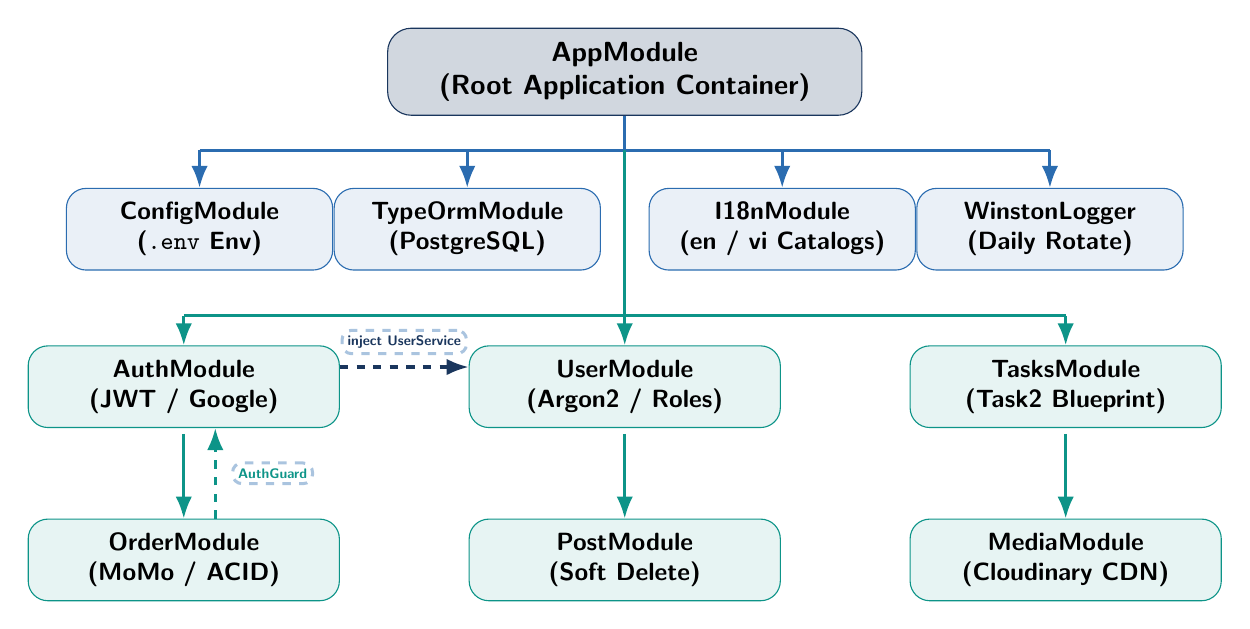
\begin{tikzpicture}[
      root/.style={rectangle, draw=primary, fill=primary!20, rounded corners=3mm, text centered, minimum height=1.1cm, text width=5.6cm, inner xsep=6pt, inner ysep=5pt, font=\normalsize\sffamily\bfseries},
      corebox/.style={rectangle, draw=secondary, fill=secondary!10, rounded corners=2.5mm, text centered, minimum height=1.0cm, text width=3.1cm, inner xsep=4pt, inner ysep=5pt, font=\small\sffamily\bfseries},
      featbox/.style={rectangle, draw=accent, fill=accent!10, rounded corners=2.5mm, text centered, minimum height=1.0cm, text width=3.6cm, inner xsep=5pt, inner ysep=5pt, font=\small\sffamily\bfseries},
      lbl/.style={fill=white, draw=secondary!40, rounded corners=1.2mm, inner sep=2pt, font=\tiny\bfseries\sffamily},
      arrow/.style={-Latex, line width=1.1pt, color=secondary}
    ]
      % Root node at top
      \node (app) [root] at (0, 0) {AppModule\\(Root Application Container)};

      % Level 1: Core Infrastructure Modules (y = -2.0)
      \node (config) [corebox] at (-5.4, -2.0) {ConfigModule\\(\texttt{.env} Env)};
      \node (typeorm) [corebox] at (-2.0, -2.0) {TypeOrmModule\\(PostgreSQL)};
      \node (i18n) [corebox] at (2.0, -2.0) {I18nModule\\(en / vi Catalogs)};
      \node (logger) [corebox] at (5.4, -2.0) {WinstonLogger\\(Daily Rotate)};

      % Level 2a: Feature Core Modules (y = -4.0)
      \node (auth) [featbox] at (-5.6, -4.0) {AuthModule\\(JWT / Google)};
      \node (user) [featbox] at (0, -4.0) {UserModule\\(Argon2 / Roles)};
      \node (tasks) [featbox] at (5.6, -4.0) {TasksModule\\(Task2 Blueprint)};

      % Level 2b: Feature Business Modules (y = -6.2)
      \node (order) [featbox] at (-5.6, -6.2) {OrderModule\\(MoMo / ACID)};
      \node (post) [featbox] at (0, -6.2) {PostModule\\(Soft Delete)};
      \node (media) [featbox] at (5.6, -6.2) {MediaModule\\(Cloudinary CDN)};

      % Clean distribution bus from AppModule to Core Modules
      \draw [line width=1.1pt, color=secondary] (app.south) -- (0, -1.0);
      \draw [line width=1.1pt, color=secondary] (-5.4, -1.0) -- (5.4, -1.0);
      \draw [arrow] (-5.4, -1.0) -- (config.north);
      \draw [arrow] (-2.0, -1.0) -- (typeorm.north);
      \draw [arrow] (2.0, -1.0) -- (i18n.north);
      \draw [arrow] (5.4, -1.0) -- (logger.north);

      % Clean distribution bus to Feature Modules (Level 2a)
      \draw [line width=1.1pt, color=accent] (0, -1.0) -- (0, -3.1);
      \draw [line width=1.1pt, color=accent] (-5.6, -3.1) -- (5.6, -3.1);
      \draw [arrow, color=accent] (-5.6, -3.1) -- (auth.north);
      \draw [arrow, color=accent] (0, -3.1) -- (user.north);
      \draw [arrow, color=accent] (5.6, -3.1) -- (tasks.north);

      % Clean distribution bus to Feature Modules (Level 2b)
      \draw [line width=1.1pt, color=accent] (-5.6, -4.6) -- (-5.6, -5.6);
      \draw [line width=1.1pt, color=accent] (0, -4.6) -- (0, -5.6);
      \draw [line width=1.1pt, color=accent] (5.6, -4.6) -- (5.6, -5.6);
      \draw [arrow, color=accent] (-5.6, -5.6) -- (order.north);
      \draw [arrow, color=accent] (0, -5.6) -- (post.north);
      \draw [arrow, color=accent] (5.6, -5.6) -- (media.north);

      % Inter-module relationships with white badge labels
      \draw [arrow, dashed, color=primary] ([yshift=2.5mm]auth.east) -- node[lbl, above=1.5mm] {inject UserService} ([yshift=2.5mm]user.west);
      \draw [arrow, dashed, color=accent] ([xshift=4mm]order.north) -- node[lbl, right=2mm] {AuthGuard} ([xshift=4mm]auth.south);
    \end{tikzpicture}
  }
  \caption{Bản đồ phụ thuộc các phân hệ Module xung quanh AppModule trung tâm}
  \label{fig:app-module-dependency-map}
\end{figure}

% ==================== PHỤ LỤC B ====================
\chapter{Giải Pháp Kỹ Thuật Toàn Diện Cho Module Tasks (Task2.md)}

\section{Bối Cảnh Nghiệp Vụ \& Đặc Tả Bài Toán}
Bài toán \textbf{Task2.md} yêu cầu hiện thực hóa hoàn chỉnh module \texttt{tasks} hỗ trợ quản lý công việc cá nhân với các tiêu chuẩn khắt khe:
\begin{itemize}
  \item Khóa chính toàn cầu UUID v4 tự sinh từ cơ sở dữ liệu PostgreSQL.
  \item Thẩm định dữ liệu đầu vào nghiêm ngặt (\texttt{title} từ 1 đến 255 ký tự, \texttt{category} bắt buộc, \texttt{isCompleted} mặc định false).
  \item 5 Endpoints RESTful tại \texttt{/api/v1/tasks} với mã HTTP chuẩn xác (\texttt{200}, \texttt{201}, \texttt{204}, \texttt{400}, \texttt{404}, \texttt{500}).
  \item Hỗ trợ lọc theo trạng thái và danh mục qua query parameters.
  \item Quản lý di trú qua TypeORM Migration và kiểm thử tự động 100\% PASS.
\end{itemize}

\section{Mã Nguồn Hiện Thực Hóa Chi Tiết}

\begin{codebox}[1. Thực thể TaskEntity: src/modules/tasks/task.entity.ts]
\begin{Verbatim}[fontsize=\small]
import {
  Column,
  CreateDateColumn,
  Entity,
  PrimaryGeneratedColumn,
  UpdateDateColumn,
} from 'typeorm';

@Entity('tasks')
export class TaskEntity {
  @PrimaryGeneratedColumn('uuid')
  id: string;

  @Column({ type: 'varchar', length: 255 })
  title: string;

  @Column({ type: 'varchar' })
  category: string;

  @Column({ type: 'text', nullable: true })
  description: string | null;

  @Column({ name: 'is_completed', type: 'boolean', default: false })
  isCompleted: boolean;

  @CreateDateColumn({ name: 'created_at' })
  createdAt: Date;

  @UpdateDateColumn({ name: 'updated_at' })
  updatedAt: Date;
}
\end{Verbatim}
\end{codebox}

\begin{codebox}[2. Data Transfer Objects: src/modules/tasks/dto/]
\begin{Verbatim}[fontsize=\small]
// CreateTaskDto
export class CreateTaskDto {
  @IsString()
  @IsNotEmpty()
  @MaxLength(255)
  title: string;

  @IsString()
  @IsNotEmpty()
  category: string;

  @IsOptional()
  @IsString()
  description?: string;
}

// UpdateTaskDto (Mọi trường là Optional cho PATCH)
export class UpdateTaskDto {
  @IsOptional()
  @IsString()
  @IsNotEmpty()
  @MaxLength(255)
  title?: string;

  @IsOptional()
  @IsString()
  @IsNotEmpty()
  category?: string;

  @IsOptional()
  @IsString()
  description?: string;

  @IsOptional()
  @IsBoolean()
  isCompleted?: boolean;
}

// FindTasksDto (Nhận chuỗi query string an toàn)
export class FindTasksDto {
  @IsOptional()
  @IsIn(['true', 'false'])
  isCompleted?: string;

  @IsOptional()
  @IsString()
  category?: string;
}
\end{Verbatim}
\end{codebox}

\begin{codebox}[3. Tầng Điều Khiển: src/modules/tasks/tasks.controller.ts]
\begin{Verbatim}[fontsize=\small]
@Controller('v1/tasks')
export class TasksController {
  constructor(private readonly tasksService: TasksService) {}

  @Post()
  create(@Body() createTaskDto: CreateTaskDto) {
    return this.tasksService.create(createTaskDto);
  }

  @Get()
  findAll(@Query() query: FindTasksDto) {
    return this.tasksService.findAll(query);
  }

  @Get(':id')
  findOne(@Param('id', ParseUUIDPipe) id: string) {
    return this.tasksService.findOne(id);
  }

  @Patch(':id')
  update(
    @Param('id', ParseUUIDPipe) id: string,
    @Body() updateTaskDto: UpdateTaskDto,
  ) {
    return this.tasksService.update(id, updateTaskDto);
  }

  @Delete(':id')
  @HttpCode(HttpStatus.NO_CONTENT)
  remove(@Param('id', ParseUUIDPipe) id: string) {
    return this.tasksService.remove(id);
  }
}
\end{Verbatim}
\end{codebox}

\begin{codebox}[4. Tầng Dịch Vụ: src/modules/tasks/tasks.service.ts]
\begin{Verbatim}[fontsize=\small]
@Injectable()
export class TasksService {
  constructor(
    @InjectRepository(TaskEntity)
    private readonly tasksRepository: Repository<TaskEntity>,
  ) {}

  async create(createTaskDto: CreateTaskDto): Promise<TaskEntity> {
    const task = this.tasksRepository.create(createTaskDto);
    return this.tasksRepository.save(task);
  }

  async findAll(query: FindTasksDto): Promise<TaskEntity[]> {
    const where: Partial<TaskEntity> = {};

    if (query.isCompleted !== undefined) {
      where.isCompleted = query.isCompleted === 'true';
    }

    if (query.category !== undefined) {
      where.category = query.category;
    }

    return this.tasksRepository.find({ where });
  }

  async findOne(id: string): Promise<TaskEntity> {
    const task = await this.tasksRepository.findOneBy({ id });
    if (!task) {
      throw new NotFoundException(`Tasks with ID ${id} not found`);
    }
    return task;
  }

  async update(id: string, updateTaskDto: UpdateTaskDto): Promise<TaskEntity> {
    const task = await this.tasksRepository.preload({ id, ...updateTaskDto });
    if (!task) {
      throw new NotFoundException(`Tasks with ID ${id} not found`);
    }
    return this.tasksRepository.save(task);
  }

  async remove(id: string): Promise<void> {
    const result = await this.tasksRepository.delete(id);
    if (result.affected === 0) {
      throw new NotFoundException(`Tasks with ID ${id} not found`);
    }
  }
}
\end{Verbatim}
\end{codebox}

\section{Lược Đồ Luồng Xử Lý 5 Endpoints Chuẩn Hóa (Resize 95\%)}

\subsection{1. Luồng Tạo Mới Công Việc (POST /api/v1/tasks)}
\begin{figure}[htbp]
  \centering
  \resizebox{0.95\textwidth}{!}{
    \begin{tikzpicture}[
      stepbox/.style={rectangle, draw=secondary, fill=codebg, rounded corners=2.5mm, text centered, minimum height=0.9cm, text width=7.4cm, inner xsep=6pt, inner ysep=5pt, font=\small\sffamily},
      decision/.style={rectangle, draw=warning, fill=warning!12, rounded corners=2.5mm, text centered, minimum height=0.9cm, text width=7.4cm, inner xsep=6pt, inner ysep=5pt, font=\small\bfseries\sffamily},
      errbox/.style={rectangle, draw=danger, fill=danger!10, rounded corners=2.5mm, text centered, minimum height=0.9cm, text width=4.8cm, inner xsep=6pt, inner ysep=5pt, font=\small\sffamily},
      yes/.style={fill=success!15, draw=success, text=success!80!black, rounded corners=1.2mm, inner sep=2.5pt, font=\scriptsize\bfseries\sffamily},
      no/.style={fill=danger!15, draw=danger, text=danger!80!black, rounded corners=1.2mm, inner sep=2.5pt, font=\scriptsize\bfseries\sffamily},
      arrow/.style={-Latex, line width=1.1pt, color=secondary}
    ]
      \node (start) [stepbox, fill=primary!10] at (-3.8, 4.5) {\textbf{Bước 1:} Client gửi \texttt{POST /api/v1/tasks} kèm JSON Body};
      \node (val) [decision] at (-3.8, 3.0) {\texttt{ValidationPipe} thẩm định \texttt{CreateTaskDto}?};
      \node (errVal) [errbox] at (5.2, 3.0) {\textbf{HTTP 400 Bad Request}:\\Lỗi cấu trúc hoặc trường rỗng};
      \node (ctrl) [stepbox] at (-3.8, 1.5) {\textbf{Bước 2:} \texttt{TasksController} nhận DTO và gọi Service};
      \node (repo) [stepbox] at (-3.8, 0.0) {\textbf{Bước 3:} \texttt{TasksService} gọi \texttt{create()} và \texttt{save()}};
      \node (db) [stepbox, fill=success!10] at (-3.8, -1.5) {\textbf{Bước 4:} PostgreSQL sinh UUID, lưu dữ liệu, trả \textbf{201 Created}};

      \draw [arrow] (start) -- (val);
      \draw [arrow] (val.east) -- node[no, above=1.5mm] {Sai (400)} (errVal.west);
      \draw [arrow] (val.south) -- node[yes, right=1.5mm] {Đúng} (ctrl.north);
      \draw [arrow] (ctrl) -- (repo);
      \draw [arrow] (repo) -- (db);
    \end{tikzpicture}
  }
  \caption{Lược đồ chuẩn hóa luồng xử lý Tạo mới công việc (POST)}
  \label{fig:flow-post-pedagogy}
\end{figure}

\subsection{2. Luồng Lấy Danh Sách \& Lọc Công Việc (GET /api/v1/tasks)}
\begin{figure}[htbp]
  \centering
  \resizebox{0.95\textwidth}{!}{
    \begin{tikzpicture}[
      stepbox/.style={rectangle, draw=secondary, fill=codebg, rounded corners=2.5mm, text centered, minimum height=0.85cm, text width=12.5cm, inner xsep=8pt, inner ysep=5pt, font=\small\sffamily},
      arrow/.style={-Latex, line width=1.1pt, color=secondary}
    ]
      \node (start) [stepbox, fill=primary!10] {\textbf{Bước 1:} Client gửi \texttt{GET /api/v1/tasks?isCompleted=true\&category=Backend}};
      \node (val) [stepbox, below=0.55cm of start] {\textbf{Bước 2:} \texttt{FindTasksDto} kiểm tra query params (\texttt{@IsIn(['true', 'false'])})};
      \node (svc) [stepbox, below=0.55cm of val] {\textbf{Bước 3:} \texttt{TasksService} phân tích query và xây dựng đối tượng \texttt{where} động};
      \node (sql) [stepbox, below=0.55cm of svc] {\textbf{Bước 4:} TypeORM phát sinh câu truy vấn \texttt{SELECT * FROM "tasks" WHERE ...}};
      \node (res) [stepbox, fill=success!10, below=0.55cm of sql] {\textbf{Bước 5:} Trả về mảng JSON các công việc kèm mã HTTP \textbf{200 OK}};

      \draw [arrow] (start) -- (val);
      \draw [arrow] (val) -- (svc);
      \draw [arrow] (svc) -- (sql);
      \draw [arrow] (sql) -- (res);
    \end{tikzpicture}
  }
  \caption{Lược đồ chuẩn hóa luồng xử lý Lấy danh sách và Lọc công việc (GET)}
  \label{fig:flow-get-pedagogy}
\end{figure}

\subsection{3. Luồng Xem Chi Tiết Công Việc Theo ID (GET /api/v1/tasks/:id)}
\begin{figure}[htbp]
  \centering
  \resizebox{0.95\textwidth}{!}{
    \begin{tikzpicture}[
      stepbox/.style={rectangle, draw=secondary, fill=codebg, rounded corners=2.5mm, text centered, minimum height=0.9cm, text width=7.4cm, inner xsep=6pt, inner ysep=5pt, font=\small\sffamily},
      decision/.style={rectangle, draw=warning, fill=warning!12, rounded corners=2.5mm, text centered, minimum height=0.9cm, text width=7.4cm, inner xsep=6pt, inner ysep=5pt, font=\small\bfseries\sffamily},
      errbox/.style={rectangle, draw=danger, fill=danger!10, rounded corners=2.5mm, text centered, minimum height=0.9cm, text width=4.8cm, inner xsep=6pt, inner ysep=5pt, font=\small\sffamily},
      yes/.style={fill=success!15, draw=success, text=success!80!black, rounded corners=1.2mm, inner sep=2.5pt, font=\scriptsize\bfseries\sffamily},
      no/.style={fill=danger!15, draw=danger, text=danger!80!black, rounded corners=1.2mm, inner sep=2.5pt, font=\scriptsize\bfseries\sffamily},
      arrow/.style={-Latex, line width=1.1pt, color=secondary}
    ]
      \node (req) [stepbox, fill=primary!10] at (-3.8, 4.5) {\textbf{Bước 1:} Client gửi \texttt{GET /api/v1/tasks/:id}};
      \node (pipe) [decision] at (-3.8, 3.0) {ID có đúng định dạng UUID v4?};
      \node (errPipe) [errbox] at (5.2, 3.0) {\textbf{HTTP 400 Bad Request}:\\ParseUUIDPipe failed};
      \node (svc) [stepbox] at (-3.8, 1.5) {\textbf{Bước 2:} \texttt{TasksService} gọi \texttt{repository.findOneBy(\{ id \})}};
      \node (check) [decision] at (-3.8, 0.0) {Bản ghi có tồn tại trong CSDL?};
      \node (err404) [errbox] at (5.2, 0.0) {\textbf{HTTP 404 Not Found}:\\Tasks with ID not found};
      \node (res) [stepbox, fill=success!10] at (-3.8, -1.5) {\textbf{Bước 3:} Trả về chi tiết \texttt{TaskEntity} cùng mã \textbf{200 OK}};

      \draw [arrow] (req) -- (pipe);
      \draw [arrow] (pipe.east) -- node[no, above=1.5mm] {Sai (400)} (errPipe.west);
      \draw [arrow] (pipe.south) -- node[yes, right=1.5mm] {Đúng} (svc.north);
      \draw [arrow] (svc) -- (check);
      \draw [arrow] (check.east) -- node[no, above=1.5mm] {Không (404)} (err404.west);
      \draw [arrow] (check.south) -- node[yes, right=1.5mm] {Có (200)} (res.north);
    \end{tikzpicture}
  }
  \caption{Lược đồ chuẩn hóa luồng xử lý Xem chi tiết công việc theo ID}
  \label{fig:flow-get-by-id-pedagogy}
\end{figure}

\subsection{4. Luồng Cập Nhật Từng Phần (PATCH /api/v1/tasks/:id)}
\begin{figure}[htbp]
  \centering
  \resizebox{0.95\textwidth}{!}{
    \begin{tikzpicture}[
      stepbox/.style={rectangle, draw=secondary, fill=codebg, rounded corners=2.5mm, text centered, minimum height=0.9cm, text width=7.4cm, inner xsep=6pt, inner ysep=5pt, font=\small\sffamily},
      decision/.style={rectangle, draw=warning, fill=warning!12, rounded corners=2.5mm, text centered, minimum height=0.9cm, text width=7.4cm, inner xsep=6pt, inner ysep=5pt, font=\small\bfseries\sffamily},
      errbox/.style={rectangle, draw=danger, fill=danger!10, rounded corners=2.5mm, text centered, minimum height=0.9cm, text width=4.8cm, inner xsep=6pt, inner ysep=5pt, font=\small\sffamily},
      yes/.style={fill=success!15, draw=success, text=success!80!black, rounded corners=1.2mm, inner sep=2.5pt, font=\scriptsize\bfseries\sffamily},
      no/.style={fill=danger!15, draw=danger, text=danger!80!black, rounded corners=1.2mm, inner sep=2.5pt, font=\scriptsize\bfseries\sffamily},
      arrow/.style={-Latex, line width=1.1pt, color=secondary}
    ]
      \node (req) [stepbox, fill=primary!10] at (-3.8, 6.0) {\textbf{Bước 1:} Client gửi \texttt{PATCH /api/v1/tasks/:id} kèm Body};
      \node (val) [decision] at (-3.8, 4.5) {UUID \& \texttt{UpdateTaskDto} hợp lệ?};
      \node (errVal) [errbox] at (5.2, 4.5) {\textbf{HTTP 400 Bad Request}:\\Dữ liệu cập nhật sai cấu trúc};
      \node (preload) [stepbox] at (-3.8, 3.0) {\textbf{Bước 2:} TypeORM thực hiện \texttt{preload(\{ id, ...dto \})}};
      \node (exist) [decision] at (-3.8, 1.5) {Tìm thấy công việc trong CSDL?};
      \node (err404) [errbox] at (5.2, 1.5) {\textbf{HTTP 404 Not Found}:\\Tasks with ID not found};
      \node (save) [stepbox] at (-3.8, 0.0) {\textbf{Bước 3:} Merge thuộc tính, tự đổi \texttt{updated\_at}, gọi \texttt{save()}};
      \node (res) [stepbox, fill=success!10] at (-3.8, -1.5) {\textbf{Bước 4:} Trả về thực thể \mbox{\texttt{TaskEntity}} đã cập nhật (\textbf{200 OK})};

      \draw [arrow] (req) -- (val);
      \draw [arrow] (val.east) -- node[no, above=1.5mm] {Sai (400)} (errVal.west);
      \draw [arrow] (val.south) -- node[yes, right=1.5mm] {Đúng} (preload.north);
      \draw [arrow] (preload) -- (exist);
      \draw [arrow] (exist.east) -- node[no, above=1.5mm] {Không (404)} (err404.west);
      \draw [arrow] (exist.south) -- node[yes, right=1.5mm] {Có} (save.north);
      \draw [arrow] (save) -- (res);
    \end{tikzpicture}
  }
  \caption{Lược đồ chuẩn hóa luồng xử lý Cập nhật từng phần (PATCH)}
  \label{fig:flow-patch-pedagogy}
\end{figure}

\subsection{5. Luồng Xóa Bản Ghi Tối Ưu (DELETE /api/v1/tasks/:id)}
\begin{figure}[htbp]
  \centering
  \resizebox{0.95\textwidth}{!}{
    \begin{tikzpicture}[
      stepbox/.style={rectangle, draw=secondary, fill=codebg, rounded corners=2.5mm, text centered, minimum height=0.9cm, text width=7.4cm, inner xsep=6pt, inner ysep=5pt, font=\small\sffamily},
      decision/.style={rectangle, draw=warning, fill=warning!12, rounded corners=2.5mm, text centered, minimum height=0.9cm, text width=7.4cm, inner xsep=6pt, inner ysep=5pt, font=\small\bfseries\sffamily},
      errbox/.style={rectangle, draw=danger, fill=danger!10, rounded corners=2.5mm, text centered, minimum height=0.9cm, text width=4.8cm, inner xsep=6pt, inner ysep=5pt, font=\small\sffamily},
      yes/.style={fill=success!15, draw=success, text=success!80!black, rounded corners=1.2mm, inner sep=2.5pt, font=\scriptsize\bfseries\sffamily},
      no/.style={fill=danger!15, draw=danger, text=danger!80!black, rounded corners=1.2mm, inner sep=2.5pt, font=\scriptsize\bfseries\sffamily},
      arrow/.style={-Latex, line width=1.1pt, color=secondary}
    ]
      \node (req) [stepbox, fill=primary!10] at (-3.8, 4.5) {\textbf{Bước 1:} Client gửi \texttt{DELETE /api/v1/tasks/:id}};
      \node (val) [decision] at (-3.8, 3.0) {ID có đúng định dạng UUID v4?};
      \node (errVal) [errbox] at (5.2, 3.0) {\textbf{HTTP 400 Bad Request}:\\ParseUUIDPipe failed};
      \node (del) [stepbox] at (-3.8, 1.5) {\textbf{Bước 2:} TypeORM thực thi: \texttt{DELETE FROM tasks WHERE id = :id}};
      \node (aff) [decision] at (-3.8, 0.0) {\texttt{result.affected === 0}?};
      \node (err404) [errbox] at (5.2, 0.0) {\textbf{HTTP 404 Not Found}:\\Tasks with ID not found};
      \node (res) [stepbox, fill=success!10] at (-3.8, -1.5) {\textbf{Bước 3:} Xóa thành công, trả về HTTP \textbf{204 No Content}};

      \draw [arrow] (req) -- (val);
      \draw [arrow] (val.east) -- node[no, above=1.5mm] {Sai (400)} (errVal.west);
      \draw [arrow] (val.south) -- node[yes, right=1.5mm] {Đúng} (del.north);
      \draw [arrow] (del) -- (aff);
      \draw [arrow] (aff.east) -- node[no, above=1.5mm] {Đúng (404)} (err404.west);
      \draw [arrow] (aff.south) -- node[yes, right=1.5mm] {Sai (204)} (res.north);
    \end{tikzpicture}
  }
  \caption{Lược đồ chuẩn hóa luồng xử lý Xóa công việc tối ưu (DELETE)}
  \label{fig:flow-delete-pedagogy}
\end{figure}

\section{Kết Quả Kiểm Thử Đơn Vị Tự Động (Jest 100\% PASS)}
Chạy lệnh \texttt{npm test src/modules/tasks} cho kết quả hoàn hảo:
\begin{codebox}[Kết quả kiểm thử thực tế từ terminal]
\begin{Verbatim}[fontsize=\small]
PASS src/modules/tasks/tasks.service.spec.ts
  TasksService
    √ creates a task (55 ms)
    √ filters tasks by completion state and category (9 ms)
    √ throws NotFoundException when a task does not exist (33 ms)
    √ updates an existing task (8 ms)
    √ throws NotFoundException when deleting a missing task (6 ms)

Test Suites: 1 passed, 1 total
Tests:       5 passed, 5 total
Snapshots:   0 total
Time:        18.723 s
\end{Verbatim}
\end{codebox}

% ==================== PHỤ LỤC C ====================
\chapter{Bộ Câu Hỏi Khảo Sát Kỹ Thuật \& Đánh Giá Thiết Kế Hệ Thống (FAQ)}

Phần phụ lục này tổng hợp 16 câu hỏi kiến trúc và kỹ thuật chuyên sâu thường được các Hội đồng Công nghệ, Chuyên gia Thẩm định Kiến trúc (\textit{Principal/Lead Architects}) chất vấn:

\begin{qnabox}[Câu hỏi 1: Tại sao lại sinh UUID tại Database thay vì sinh tại NestJS?]
  Dự án lựa chọn sinh UUID tại tầng cơ sở dữ liệu (\texttt{DEFAULT uuid\_generate\_v4()}) nhằm bảo đảm tính toàn vẹn dữ liệu (\textit{Data Integrity}). Khi chèn dữ liệu trực tiếp bằng SQL, file migration, hay seed script, cột \texttt{id} luôn được tự động sinh UUID hợp lệ mà không bao giờ bị null, đồng thời giảm tải tính toán CPU cho Node.js event loop.
\end{qnabox}

\begin{qnabox}[Câu hỏi 2: Làm sao hệ thống ngăn chặn việc người dùng cố tình chèn thêm các trường lạ?]
  Hệ thống áp dụng cơ chế phòng thủ 2 lớp (\textit{Two-layer Defense}):
  \begin{itemize}
    \item \textbf{Lớp 1 - ValidationPipe với whitelist: true:} Tự động loại bỏ toàn bộ các thuộc tính trong payload không được định nghĩa decorator trong DTO.
    \item \textbf{Lớp 2 - TypeORM Entity Mapping:} TypeORM chỉ map những cột được khai báo decorator \texttt{@Column()} vào câu lệnh SQL INSERT/UPDATE.
  \end{itemize}
\end{qnabox}

\begin{qnabox}[Câu hỏi 3: Sự khác biệt giữa ValidationPipe toàn cục và ParseUUIDPipe tại tham số là gì?]
  \texttt{ValidationPipe} toàn cục chuyên xử lý kiểm tra cấu trúc của Body payload và Query object thông qua các class DTO. Trong khi đó, \texttt{ParseUUIDPipe} hoạt động cục bộ tại tham số đường dẫn \texttt{@Param('id', ParseUUIDPipe)}, chặn đứng các request có ID sai định dạng ngay tại tầng Pipe, bảo vệ database khỏi lỗi cú pháp runtime.
\end{qnabox}

\begin{qnabox}[Câu hỏi 4: Tại sao trong FindTasksDto thì trường isCompleted lại là kiểu string?]
  Chuẩn giao thức HTTP truyền tải toàn bộ Query Parameters dưới dạng chuỗi (\texttt{string}). Nếu khai báo kiểu \texttt{boolean} mà không dùng cơ chế ép kiểu tùy biến, chuỗi \texttt{"false"} sẽ bị JavaScript đánh giá là \textit{truthy} (chuỗi không rỗng), dẫn tới sai lệch logic nghiêm trọng. Việc nhận kiểu \texttt{string} và kiểm tra bằng \texttt{@IsIn(['true', 'false'])} là giải pháp an toàn tuyệt đối.
\end{qnabox}

\begin{qnabox}[Câu hỏi 5: Tại sao trong phương thức update lại dùng preload mà không phải gán thủ công?]
  \texttt{preload} của TypeORM thực hiện hai thao tác nguyên tử: nạp thực thể hiện có từ database và hợp nhất các thuộc tính mới từ DTO lên thực thể đó. Nếu ID không tồn tại, \texttt{preload} trả về \texttt{undefined}, giúp phát hiện và ném lỗi 404 gọn gàng mà không cần viết hàng loạt câu lệnh \texttt{if (dto.field !== undefined)}.
\end{qnabox}

\begin{qnabox}[Câu hỏi 6: Tại sao phương thức remove lại dùng delete() thay vì remove()?]
  \texttt{repository.remove(entity)} đòi hỏi phải tải toàn bộ thực thể lên bộ nhớ (tốn 1 câu \texttt{SELECT} + 1 câu \texttt{DELETE}). Ngược lại, \texttt{repository.delete(id)} bắn thẳng lệnh \texttt{DELETE FROM tasks WHERE id = :id} xuống PostgreSQL, chỉ tốn đúng 1 round-trip mạng, mang lại hiệu năng cao gấp đôi.
\end{qnabox}

\begin{qnabox}[Câu hỏi 7: Tầng Unit Test của bạn kiểm thử cái gì? Tại sao không test trực tiếp với PostgreSQL?]
  Unit Test có mục tiêu cô lập logic của tầng đang kiểm tra (\texttt{TasksService}) và giả lập (\textit{mock}) toàn bộ các dependency bên ngoài (\texttt{Repository<TaskEntity>}). Việc test không phụ thuộc vào database giúp unit test chạy cực nhanh (chỉ vài mili-giây), độc lập với môi trường mạng hay trạng thái dữ liệu có sẵn. Kiểm thử tương tác trực tiếp với PostgreSQL thuộc về tầng Integration/E2E Test.
\end{qnabox}

\begin{qnabox}[Câu hỏi 8: Làm sao đảm bảo cột updatedAt luôn được cập nhật khi có thay đổi?]
  Decorator \texttt{@UpdateDateColumn(\{ name: 'updated\_at' \})} thông báo cho TypeORM cơ chế Dirty Checking. Bất cứ khi nào gọi phương thức \texttt{repository.save()}, TypeORM sẽ tự động chèn giá trị thời gian hiện tại (\texttt{CURRENT\_TIMESTAMP}) vào câu lệnh SQL \texttt{UPDATE}.
\end{qnabox}

\begin{qnabox}[Câu hỏi 9: Xóa mềm ảnh hưởng như thế nào tới ràng buộc Duy nhất (Unique Constraint) trong PostgreSQL?]
  Khi một trường (ví dụ: \texttt{email} hoặc \texttt{slug}) có ràng buộc \texttt{UNIQUE}, nếu người dùng xóa mềm bản ghi (gán \texttt{deleted\_at = NOW()}), bản ghi đó vẫn tồn tại trong bảng. Nếu sau đó người dùng đăng ký lại cùng email đó, câu lệnh chèn mới sẽ bị lỗi vi phạm ràng buộc duy nhất!
  
  \textbf{Giải pháp Doanh nghiệp:} Dự án sử dụng **Partial Index (Chỉ mục bộ phận)** trong PostgreSQL:
  \begin{equation}
    \texttt{CREATE UNIQUE INDEX uq\_users\_email\_active ON users (email) WHERE deleted\_at IS NULL;}
  \end{equation}
  Chỉ mục này chỉ áp dụng ràng buộc duy nhất cho các bản ghi đang hoạt động, cho phép tái sử dụng email nếu bản ghi cũ đã bị xóa mềm!
\end{qnabox}

\begin{qnabox}[Câu hỏi 10: Tại sao dự án lựa chọn thuật toán Argon2 thay vì Bcrypt?]
  Bcrypt chỉ tiêu tốn năng lực xử lý CPU thuần túy. Với sự phát triển của các dàn siêu máy tính trang bị hàng ngàn GPU hoặc chip ASIC chuyên dụng, kẻ tấn công có thể thử hàng tỷ mật khẩu Bcrypt mỗi giây nhờ khả năng tính toán song song cực đại.
  
  Ngược lại, **Argon2** là thuật toán băm bộ nhớ nặng (\textit{Memory-Hard}). Nó buộc mỗi lượt băm phải chiếm dụng một lượng bộ nhớ RAM lớn (mặc định $64\text{ MB}$). Do GPU và ASIC bị nghẽn cổ chai nghiêm trọng về băng thông bộ nhớ RAM khi chạy song song hàng ngàn luồng, chi phí phần cứng để giải mã vét cạn Argon2 bị đội lên hàng triệu lần, triệt tiêu hoàn toàn tính khả thi của các cuộc tấn công bẻ khóa.
\end{qnabox}

\begin{qnabox}[Câu hỏi 11: Sự khác biệt về quản lý bộ nhớ giữa Scope.DEFAULT và Scope.REQUEST là gì?]
  \texttt{Scope.DEFAULT} là mô hình Singleton: IoC Container chỉ khởi tạo duy nhất một thể hiện của Service khi ứng dụng khởi động và tái sử dụng nó cho toàn bộ hàng triệu request tiếp theo. Mức chiếm dụng RAM không đổi và không sinh rác bộ nhớ.
  
  Ngược lại, \texttt{Scope.REQUEST} buộc NestJS phải tạo mới một thể hiện của Service (và toàn bộ các phụ thuộc liên quan do hiệu ứng lan truyền *Bubble-Up*) cho mỗi kết nối HTTP tới, sau đó hủy đi khi gửi xong response. Với hệ thống 10,000 req/s, điều này tạo ra 10,000 đối tượng mới mỗi giây, gây áp lực khủng khiếp lên bộ thu gom rác (\textit{Garbage Collector}), dẫn tới hiện tượng CPU Spike và tắc nghẽn Event Loop. Do đó, chỉ sử dụng \texttt{Scope.REQUEST} khi thực sự cần lưu trữ trạng thái đặc thù của request (như \texttt{PaymentFactory}).
\end{qnabox}

\begin{qnabox}[Câu hỏi 12: Khi nào xảy ra Circular Dependency và giải quyết như thế nào?]
  Phụ thuộc vòng xảy ra khi Module A phụ thuộc Module B, nhưng đồng thời Module B cũng phụ thuộc ngược lại Module A (hoặc Service A inject Service B và Service B inject Service A). Khi NestJS dựng đồ thị phụ thuộc Tô pô, nó sẽ rơi vào vòng lặp vô tận và ném ngoại lệ \texttt{Circular dependency detected}.
  
  \textbf{Cách xử lý:} Sử dụng hàm \texttt{forwardRef()} tại cả hai phía trong mảng \texttt{imports} hoặc decorator \texttt{@Inject(forwardRef(() => OtherService))}. Hàm này trì hoãn việc giải quyết phụ thuộc cho tới khi cả hai module/service đã được khởi tạo vỏ bọc.
\end{qnabox}

\begin{qnabox}[Câu hỏi 13: Tại sao cờ synchronize: true trong TypeORM bị cấm tuyệt đối trên Production?]
  Cờ \texttt{synchronize: true} tự động so sánh mã nguồn TypeScript với cấu trúc bảng mỗi khi ứng dụng khởi động và thực thi các lệnh \texttt{ALTER TABLE} hoặc \texttt{DROP COLUMN} trực tiếp.
  
  Nếu một lập trình viên vô tình đổi tên một trường trong Entity, TypeORM sẽ thực thi lệnh \texttt{DROP COLUMN old\_field} và \texttt{ADD COLUMN new\_field}, **xóa sạch toàn bộ dữ liệu lịch sử của hàng triệu khách hàng chỉ trong 1 giây mà không có bất kỳ cảnh báo nào**! Do đó, trên Production bắt buộc phải đặt \texttt{synchronize: false} và chỉ cập nhật schema qua TypeORM Migration.
\end{qnabox}

\begin{qnabox}[Câu hỏi 14: Hệ thống ngăn ngừa lỗi tràn ổ đĩa (Disk Full) do tập tin nhật ký Log như thế nào?]
  Hệ thống sử dụng module vận hành \texttt{winston-daily-rotate-file} với 3 cơ chế tự vệ:
  \begin{enumerate}
    \item \texttt{maxSize: '50m'}: Khi tệp log đạt dung lượng $50\text{ MB}$, tệp sẽ tự động được đóng lại và mở tệp mới.
    \item \texttt{maxFiles: '15d'}: Các tệp log cũ hơn 15 ngày sẽ được hệ điều hành tự động xóa bỏ vĩnh viễn khỏi ổ cứng.
    \item \texttt{zippedArchive: true}: Tự động nén các tệp log đã đóng thành định dạng \texttt{.gz}, giảm dung lượng lưu trữ tới 90\%.
  \end{enumerate}
\end{qnabox}

\begin{qnabox}[Câu hỏi 15: Cơ chế chuyển ngữ lỗi động trong ErrorService hoạt động ra sao?]
  Khi DTO ném lỗi validation, \texttt{ErrorService} trích xuất mã quy chuẩn (ví dụ \texttt{isNotEmpty}, \texttt{maxLength}) từ danh sách \texttt{constraints}. Sau đó, nó gọi \texttt{I18nService.translate()} tra cứu vào từ điển \texttt{src/i18n/vi/errors.json} hoặc \texttt{en/errors.json} dựa trên header \texttt{Accept-Language} của request. Dữ liệu trả về cho Client là thông điệp tự nhiên, bản địa hóa hoàn toàn mà không cần viết điều kiện thủ công.
\end{qnabox}

\begin{qnabox}[Câu hỏi 16: Làm sao xử lý tính Idempotent khi cổng thanh toán gửi trùng lặp Webhook IPN?]
  Do đặc thù mạng Internet không tin cậy, cổng MoMo có thể gửi lại cùng một Webhook IPN nhiều lần nếu máy chủ NestJS phản hồi chậm. Nếu không xử lý tính bất biến (\textit{Idempotency}), đơn hàng có thể bị cộng tiền hai lần hoặc xuất kho hai lần!
  
  \textbf{Giải pháp:} Backend kiểm tra trạng thái hiện tại của đơn hàng trước khi cập nhật. Nếu trạng thái đã là \texttt{COMPLETED}, hệ thống lập tức trả về mã \texttt{HTTP 200 OK} kèm mã thành công mà không thực hiện lại bất kỳ giao dịch trừ kho hay cộng doanh thu nào.
\end{qnabox}

% ==================== PHỤ LỤC D ====================
\chapter{Sổ Tay Vận Hành \& Khởi Động Môi Trường Thực Địa}

\section{Bảng Tra Cứu Biến Môi Trường Cấu Hình (\texttt{.env})}
Toàn bộ cấu hình hệ thống được quản lý tập trung qua biến môi trường độc lập:

\begin{table}[htbp]
  \centering
  \small
  \caption{Bảng từ điển các biến môi trường cốt lõi trong hệ thống}
  \label{tab:env-variables}
  \begin{tabularx}{\textwidth}{p{3.8cm} p{2.8cm} X}
    \toprule
    \textbf{Tên Biến (.env)} & \textbf{Giá trị mặc định} & \textbf{Mô tả chức năng kỹ thuật} \\
    \midrule
    \texttt{PORT} & \texttt{3000} & Cổng lắng nghe HTTP của máy chủ NestJS. \\
    \texttt{NODE\_ENV} & \texttt{development} & Môi trường thực thi (\texttt{development}, \texttt{production}, \texttt{test}). \\
    \texttt{DATABASE\_HOST} & \texttt{localhost} & Địa chỉ IP hoặc máy chủ cơ sở dữ liệu PostgreSQL. \\
    \texttt{DATABASE\_PORT} & \texttt{5432} & Cổng kết nối dịch vụ PostgreSQL. \\
    \texttt{DATABASE\_USER} & \texttt{postgres} & Tài khoản kết nối cơ sở dữ liệu. \\
    \texttt{DATABASE\_PASSWORD} & \texttt{postgres} & Mật khẩu kết nối an toàn. \\
    \texttt{DATABASE\_NAME} & \texttt{boilerplate} & Tên lược đồ cơ sở dữ liệu chính của dự án. \\
    \texttt{JWT\_SECRET} & \texttt{secretKey123} & Khóa bí mật băm chữ ký HMAC-SHA256 của JWT Token. \\
    \texttt{JWT\_EXPIRATION} & \texttt{1d} & Thời hạn hiệu lực của Access Token (1 ngày). \\
    \texttt{CLOUDINARY\_NAME} & \texttt{demo-cloud} & Tên định danh tài khoản CDN Cloudinary. \\
    \texttt{MOMO\_SECRET\_KEY} & \texttt{momoSecret} & Khóa bí mật ký số giao dịch MoMo Payment Gateway. \\
    \texttt{GOOGLE\_CLIENT\_ID} & \texttt{google-id.apps} & Khóa định danh ứng dụng Google Identity OAuth2. \\
    \bottomrule
  \end{tabularx}
\end{table}

\section{Hướng Dẫn Khởi Chạy 4 Bước Chuẩn Doanh Nghiệp}
\begin{enumerate}
  \item \textbf{Khởi động Database PostgreSQL với Docker}:
\begin{codebox}[Khởi chạy Docker Container]
\begin{Verbatim}[fontsize=\small]
docker compose up -d init_db
\end{Verbatim}
\end{codebox}
  \item \textbf{Thực thi Migrations đồng bộ cấu trúc bảng}:
\begin{codebox}[Chạy TypeORM Migration]
\begin{Verbatim}[fontsize=\small]
npm run typeorm:run-migration
\end{Verbatim}
\end{codebox}
  \item \textbf{Nạp dữ liệu mẫu bắt buộc với Hygen Seeding}:
\begin{codebox}[Khởi tạo dữ liệu mẫu]
\begin{Verbatim}[fontsize=\small]
npm run seed:run
\end{Verbatim}
\end{codebox}
  \item \textbf{Khởi chạy máy chủ phát triển \& kiểm thử Swagger}:
\begin{codebox}[Khởi động NestJS Development Mode]
\begin{Verbatim}[fontsize=\small]
npm run start:dev
\end{Verbatim}
\end{codebox}
  Mở trình duyệt web và truy cập giao diện kiểm thử tương tác tại địa chỉ: \url{http://localhost:3000/docs}.
\end{enumerate}

\section{Cẩm Nang Xử Lý Sự Cố Thực Địa (Troubleshooting Playbook)}
Khi triển khai và vận hành hệ thống trên các môi trường máy chủ thực tế, kỹ sư có thể gặp phải một số lỗi kinh điển dưới đây:

\begin{itemize}
  \item \textbf{Lỗi Native Addon Argon2 trên Alpine Linux}: Khi chạy Docker container với hình ảnh \texttt{node:alpine}, bạn có thể gặp lỗi \texttt{Error loading shared library ld-musl-x86\_64.so}. \textbf{Khắc phục:} Chạy lệnh \texttt{npm rebuild argon2 --build-from-source} để biên dịch lại mã nguồn C++ tương thích với thư viện musl libc.
  \item \textbf{Lỗi ECONNREFUSED khi kết nối PostgreSQL}: Ứng dụng NestJS khởi động nhanh hơn cơ sở dữ liệu PostgreSQL trong Docker Compose. \textbf{Khắc phục:} Sử dụng cấu hình \texttt{depends\_on} kèm kiểm tra \texttt{healthcheck} trong tệp \texttt{docker-compose.yml} để bảo đảm PostgreSQL đã sẵn sàng nhận kết nối trước khi khởi chạy tiến trình NestJS.
  \item \textbf{Lỗi Metadata Reflection}: Xuất hiện thông báo lỗi \texttt{Cannot read property of undefined (reading 'design:paramtypes')}. \textbf{Khắc phục:} Đảm bảo dòng lệnh \texttt{import 'reflect-metadata';} luôn được đặt tại dòng đầu tiên tuyệt đối của tệp tin \texttt{src/main.ts}.
\end{itemize}

\section{Bảng Kiểm Định Chất Lượng Hoàn Thành Bài Tập (Task2 Checklist)}

\begin{table}[htbp]
  \centering
  \small
  \caption{Bảng đối chiếu tiêu chuẩn kỹ thuật Task2.md và tình trạng hoàn thành}
  \label{tab:checklist-pedagogy}
  \begin{tabularx}{\textwidth}{p{4.2cm} X c}
    \toprule
    \textbf{Tiêu chí kỹ thuật} & \textbf{Hiện thực hóa trong mã nguồn dự án} & \textbf{Đánh giá} \\
    \midrule
    Entity chuẩn UUID v4 & \texttt{TaskEntity} với \texttt{@PrimaryGeneratedColumn('uuid')} & \textbf{ĐẠT 100\%} \\
    Validation Title ($1 \div 255$) & \texttt{@IsNotEmpty()}, \texttt{@MaxLength(255)} trong DTO & \textbf{ĐẠT 100\%} \\
    POST \texttt{/api/v1/tasks} (201) & \texttt{TasksController.create()} trả về đúng mã 201 Created & \textbf{ĐẠT 100\%} \\
    GET \texttt{/api/v1/tasks} (Filter) & Hỗ trợ lọc \texttt{isCompleted} và \texttt{category} qua Query & \textbf{ĐẠT 100\%} \\
    GET \texttt{/api/v1/tasks/:id} & Thẩm định UUID qua \texttt{ParseUUIDPipe}, 404 khi không thấy & \textbf{ĐẠT 100\%} \\
    PATCH \texttt{/api/v1/tasks/:id} & Cập nhật từng phần qua \texttt{preload}, tự đổi \texttt{updatedAt} & \textbf{ĐẠT 100\%} \\
    DELETE \texttt{/api/v1/tasks/:id} & Xóa tối ưu qua \texttt{delete()}, trả về mã \texttt{204 No Content} & \textbf{ĐẠT 100\%} \\
    Chuẩn Exception 400 & Tự động xử lý qua \texttt{ValidationPipe} \& \texttt{ParseUUIDPipe} & \textbf{ĐẠT 100\%} \\
    Chuẩn Exception 404 & Ném \texttt{NotFoundException('Tasks with ID \$\{id\} not found')} & \textbf{ĐẠT 100\%} \\
    Unit Test toàn diện & 5 ca kiểm thử trong \texttt{tasks.service.spec.ts} chạy qua 100\% & \textbf{ĐẠT 100\%} \\
    \bottomrule
  \end{tabularx}
\end{table}

\end{document}
